% MDPI MAKE53: native-pruning validation and controlled empirical scope.
\documentclass[make,article,submit,pdftex,moreauthors]{Definitions/mdpi}

%=================================================================
% MDPI internal commands — do not modify
\firstpage{1}
\makeatletter
\setcounter{page}{\@firstpage}
\makeatother
\pubvolume{8}
\issuenum{1}
\articlenumber{0}
\pubyear{2026}
\copyrightyear{2026}
%\externaleditor{Firstname Lastname}
\datereceived{ }
\daterevised{ }
\dateaccepted{ }
\datepublished{ }

%=================================================================
% Notation shorthands
\newcommand{\dID}{d_{\mathrm{ID}}}
\newcommand{\hatdID}{\hat{d}_{\mathrm{ID}}}
\newcommand{\dz}{m}
\newcommand{\dtrue}{d_{\mathrm{true}}}
\newcommand{\Jg}{J_g}
\newcommand{\R}{\mathbb{R}}
\newcommand{\kap}{\kappa}
\newcommand{\AUsat}{\mathrm{AU}_{\mathrm{sat}}}
\newcommand{\demb}{d_{\mathrm{emb}}}
\newcommand{\mknee}{m^{\mathrm{knee}}}
\newcommand{\dstar}{d^{*}(\beta)}

%=================================================================
\Title{Intrinsic-Dimension-Guided Bottleneck Selection for
Variational Autoencoders with Active-Unit Diagnostics}

% ORCID IDs
\newcommand{\orcidauthorA}{0009-0001-1209-0918} % Chika Obata
\newcommand{\orcidauthorB}{0000-0002-4070-4585} % Mizuki Dai
\newcommand{\orcidauthorC}{0000-0002-0431-5769} % Kenya Jin'no

\Author{Chika Obata $^{1}$\orcidA{},
        Mizuki Dai $^{1}$\orcidB{}, and
        Kenya Jin'no $^{1,}$*\orcidC{}}

\AuthorNames{Chika Obata, Mizuki Dai, and Kenya Jin'no}

\address{%
$^{1}$ \quad Department of Intelligent Systems,
  Faculty of Information Engineering,
  Tokyo City University,
  1-28-1 Tamazutsumi, Setagaya-ku, Tokyo 158-8557, Japan;
  g2332016@tcu.ac.jp (C.O.); g2591402@tcu.ac.jp (M.D.)}

\corres{Correspondence: kjinno@tcu.ac.jp; Tel.: +81-3-5707-0104 (K.J.)}

%=================================================================

% MAKE53: title continuity and native-pruning revision, 2026-09-19.
\usepackage{xurl}
\emergencystretch=1.5em
\setlength{\headheight}{20pt}
\abstract{%
Intrinsic-dimension estimates and active-unit diagnostics address different
aspects of variational-autoencoder bottleneck selection. We evaluate
search policies on four image datasets, five training seeds and five
regularisation weights, using a validation quality target and common
recorded candidate costs. A start-width ablation holds reliability checks,
fallback and reference-bank charges fixed. ID is accepted only for the
25 MNIST conditions: ID-derived and gated midpoint starts select the
same widths, requesting 8.84 and 5.84 candidates on average, respectively.
The remaining 75 conditions use the same ascending fallback. Across
10,000 replay evaluations from 100 coefficient--threshold combinations
and 100 dataset--weight--seed conditions, 155 local outputs miss the
smallest qualifying width. Three-seed pruning experiments per dataset
distinguish reconstruction by the selected native model from dimension
transfer to an ordinary variational autoencoder. In a local relevance-prior
variant, masking nonselected axes increases dSprites validation error
by 126.3\%; 30 decoder-adaptation epochs reduce this to 37.1\% above
the full model. All four evaluated conditions, including the full model,
miss that dataset's quality target. Active-unit prediction does not
establish additional benefit on its near-ceiling task. The findings
support a controlled empirical evaluation of selection rules and
diagnostics, without a general efficiency or pruning guarantee.}
\keyword{variational autoencoder; bottleneck dimension; intrinsic dimension;
active units; model selection; reconstruction quality; reproducibility}

\begin{document}
\section{Introduction}\label{sec:intro}

The latent width of a variational autoencoder (VAE)~\cite{kingma2014vae}
controls the capacity available to its representation. Choosing that width
by validation over a candidate grid is straightforward, but requires
training several models. Alternatives include intrinsic-dimension (ID)
estimation~\cite{facco2017twonn,levina2005mle}, comparisons between sampled
and mean latent representations~\cite{bonheme2022fondue}, activity
diagnostics~\cite{burda2016iwae,bonheme2023active}, and pruning through
reconstruction constraints or relevance priors~\cite{deboom2020geco,saha2025ardvae}.
These signals answer different questions: geometric dimension, coordinate
use, reconstruction quality and network width need not coincide.

This study asks how the use of ID changes the decisions and training
requests of a latent-width search, whether AU diagnostics add predictive
value beyond other recorded quantities, and how these measurements depend
on quality targets and readout settings. We compare policies on common
candidate-model families and fixed splits. Search order, stopping rules,
quality attainment and agreement with the smallest qualifying grid width
are measured separately.

The contribution is an empirical evaluation of ID-guided bottleneck
selection and AU diagnostics under explicit quality and cost definitions.
Four image datasets, five candidate seeds and five regularisation weights
are covered. A start-width ablation holds reference acquisition,
reliability checks and fallback fixed, isolating the effect of the
ID-derived start from the effect of the search rule. A factorial analysis
examines the ID coefficient and reliability thresholds.

Additional three-seed experiments on each dataset assess stochastic-gate
pruning and exact-Jacobian relevance readouts. For a local ARD variant,
we compare the full model, selected-axis masking, fixed-budget decoder
adaptation and transfer to an ordinary VAE. Component checks do not
establish full reproduction of the original pruning methods. A separate
one-seed MNIST experiment evaluates capacity selection by a Monte Carlo
estimate of the evidence lower bound (ELBO).
Sections~\ref{sec:framework}--\ref{sec:setup} define the protocols,
Section~\ref{sec:results} reports results, and
Section~\ref{sec:discussion} states the scope of inference.

\section{Related Work}\label{sec:related}

\subsection{Dimension, Reconstruction and Latent Activity}
PCA~\cite{tippingbishop1999ppca}, Isomap~\cite{tenenbaum2000isomap} and
locally linear embedding~\cite{roweis2000lle} construct low-dimensional
representations. ID estimators instead quantify local dimension from
sample geometry. We use TwoNN and an MLE cross-check; other approaches
include DANCo, expected simplex skewness and geodesic entropic
graphs~\cite{ceruti2014danco,johnsson2015ess,costa2004geodesic}.
Estimator limitations and dependence on the sampled distribution motivate
cross-checks~\cite{camastra2016intrinsic,allegra2020data}.
Graph-based methods are outside this experiment's scope; we do not infer
that they would resolve or reproduce the observed disagreements.
Minimal-spanning-tree isolation forests also use graph geometry for
anomaly scoring~\cite{galka2022isolation}; that objective is distinct from
selecting a VAE width under a reconstruction target.
Lower ID in learned representations has also been observed in deep
networks~\cite{ansuini2019intrinsic,pope2021intrinsic}.

FONDUE~\cite{bonheme2022fondue} searches for the capacity preceding a
separation between ID estimates of sampled and posterior-mean
representations. Its appendix gives FONDUE-VAR, which chooses a count from
latent-variable types. AU and variable types share an interest in unused
coordinates but are different statistics: AU thresholds the across-data
variance of posterior means, whereas the type classifier uses moments of
posterior variances~\cite{bonheme2023active}. Agreement of their final
counts is not equivalence of their stability or information content.

GECO with $L_0$ regularisation optimises a gated VAE under a reconstruction
constraint~\cite{deboom2020geco,rezende2018geco}. Its source uses ARM;
the historical local adaptation used hard-concrete (HC)
gates~\cite{louizos2018l0}. The additional ARM implementation restores
this gradient component but retains differences in initialisation,
constraint scheduling and KL scaling (Section~\ref{sec:gpuvalidation}).
Our validation anchor supplies an external quality yardstick.

ARD-VAE uses a hierarchical relevance prior~\cite{saha2025ardvae}.
The source tunes a regularisation weight, uses a Gaussian approximation
for its closed-form KL, and selects axes explaining 99\% of a
Jacobian-weighted variance score. The Gaussian approximation is thus
shared with the source. Historical finite-step scores and their
normalisation audit appear in Appendix~\ref{app:adaptations}; the new
validation uses automatic-differentiation Jacobians. We distinguish the
source's zero-centre variance update from an additional sample-centred
variance-update variant, and retain local training and sampling settings.

\subsection{Relation to the Conference Paper and Earlier Manuscript}
Our NOLTA2025 contribution~\cite{obata2025manifold} concerned the relation
between input ID and latent-space capacity. The available conference
manuscript describes class-specific MNIST experiments with four fully
connected and two convolutional architectures and four seeds. CNNs and
multiple seeds are consequently not new features of this revision.
The conference manuscript available for comparison has a working title
different from the published title; the reference uses the title and
pages listed by the authors' institutional publication record.
Table~\ref{tab:history} distinguishes this earlier scope from the present
comparison. MAKE47 denotes the earlier journal submission, not a separate
publication.

The present contribution is a controlled empirical comparison, rather
than a claim that the original heuristic is generally superior.
We withdraw the earlier 60--80\% training-call reduction as a general
efficiency claim. The earlier AU checks V1/V2 no longer decide the
selected width, and this study does not establish their additional
predictive value. Theoretical embedding considerations motivate the
experiment; they do not guarantee the numerical ID-to-width rule.

\begin{table}[H]
\caption{Scope of the conference study, earlier journal submission and present revision.}
\label{tab:history}\small
\begin{tabularx}{\textwidth}{lXXX}\toprule
Item & NOLTA2025 & MAKE47 & Present revision \\\midrule
Question & Input and latent ID versus capacity & ID-guided choice with AU verification & Selection quality, cost and diagnostic limitations \\
Models & Four FC and two CNN structures; MNIST classes; four seeds & FC/CNN and synthetic/image extensions & Fixed candidate families on four image datasets; five candidate seeds \\
Comparators & Architecture and capacity comparisons & Capacity sweeps and diagnostic checks & FONDUE variants, grid criteria and search policies; separate pruning validation \\
Readouts & ID estimates & AU-based operational checks & Same-checkpoint type/AU trajectories and paired predictive analysis \\
Evidence & Conference settings & Earlier loss convention & Corrected-loss records; explicit targets, final test metrics and accounting limits \\
\bottomrule\end{tabularx}
\end{table}

\section{Evaluation Framework}\label{sec:framework}

\subsection{Models and Quality Target}\label{sec:quality}
We distinguish the \emph{ID-reference AE}, which supplies a representation
for estimation, the \emph{quality anchor}, an ordinary VAE at the largest
candidate width, and the \emph{selected model}, the ordinary VAE evaluated
after dimension selection. Write $\mathcal M$ for the candidate grid,
$s$ for a training seed, and $D_s(m,\beta)$ for validation per-pixel MSE
of the deterministic reconstruction $g(\mu(x))$. The implemented target is
\begin{align}
 m_a&=\max\mathcal M, &
 T_{D,s}(\beta)&=D_s(m_a,\beta)
 +\max\{0.10D_s(m_a,\beta),\,0.001\operatorname{Var}(X_{\rm val})\}.
 \label{eq:target}
\end{align}
The variance is computed over all validation-array entries. The relative
term dominates in every recorded image condition, giving
$T_{D,s}=1.10D_s(m_a,\beta)$. The configuration originally also specified a
three-seed-SD term, but the executed target function was supplied one
anchor at a time and omitted that term. We report the implemented rule;
we do not retrospectively describe it as a pooled-seed target.
Appendix~\ref{app:targets} lists every dataset--$\beta$ anchor and target.

For a fixed seed and $\beta$, the target is held constant during search.
It is recomputed from a different anchor when $\beta$ changes. A
$\beta$-sweep therefore changes both the learned representation and the
quality yardstick. It is not a fixed-quality intervention. A method that
returns a valid width need not meet this external target; quality
attainment is evaluated separately for every final model.

\subsection{Canonical Replay Prices and Historical Ledgers}\label{sec:cost}
Replay uses one immutable candidate snapshot. A logical key contains
dataset, width, training seed, requested epochs, early-stopping option and
$\beta$; architecture, likelihood and split are fixed by the dataset
configuration. Each unique requested key, including the quality anchor,
is charged its duration in this snapshot once. Metrics and prices are
therefore identical whenever replay policies request the same key.
These are paired uses of stored records, not independent retraining.

Earlier method ledgers sometimes attach different durations to the same
logical key. Even when validation and test summaries agree exactly,
missing historical weights and execution identifiers prevent proving
checkpoint identity. We therefore do not mix those prices in the new
policy comparison. Appendix~\ref{app:timing} preserves the historical
account and resolves every anchor/final role to its key, source and both
available durations in a supplementary CSV. The quality anchor and its
price in each replay come from the same record.

Let $C_{\rm cand}$ sum the canonical prices of requested candidates and
$C_{\rm ref}$ be the nine-AE bank's recorded training cost.
Cold use charges $C_{\rm cand}+C_{\rm ref}$ for an ID policy; warm use
charges $C_{\rm cand}$ when that bank already exists. A 25-task batch
(five seeds by five weights for one dataset) allocates $C_{\rm ref}/25$
per task. This does not turn shared-bank outcomes into independent ID
replications. All accounts exclude missing ID-computation and some
post-training evaluation times. They estimate attributed training costs,
not new end-to-end wall-clock measurements. Historical probe and FONDUE
calibration costs are reported separately from the replay policies.

\subsection{Outputs and Termination}\label{sec:outcomes}
Each trial records a raw returned dimension, the width of the evaluated
model, the ID reliability decision where applicable, fallback use, the
logged termination state, the budget flag, quality attainment, and whether
the final width is smaller than the anchor. These events can overlap.
In particular, fallback can produce a compact model that meets the target.
The label \texttt{SUCCESS} in an older log indicates ordinary termination;
it is not itself evidence of target attainment.

A budget-exceeded trial contributes its consumed time and, if it has a
returned model, that model's dimension and metrics. A raw dimension below
one is reported as degenerate; its time and failure count remain, while
MSE is missing because no final model exists. The original implementation
checks budgets after completed calls and can still obtain a final model.
The reported limits are therefore soft accounting limits, not hard
interruptions. Outcome tables preserve these distinctions.

\subsection{Reference Bank and Reliability Checks}\label{sec:algorithm}
The reference bank uses three widths and
three fixed reference seeds, shared across the five candidate seeds.
Let $\bar d_r$ be the mean TwoNN estimate at reference width $r$,
$\hat d=\operatorname{mean}_r\bar d_r$, and $\bar d_{\rm MLE}$ the mean
MLE estimate over that same bank. The checks are
\begin{equation}
 R=\frac{\max_r\bar d_r-\min_r\bar d_r}{\operatorname{median}_r\bar d_r}
 \le0.15,\qquad
 A=\frac{|\hat d-\bar d_{\rm MLE}|}{\hat d}\le0.25.
 \label{eq:checks}
\end{equation}
The values $c=2$, $R_{\max}=0.15$ and $A_{\max}=0.25$ were internal
heuristics recorded in the 12--13 September specification. The factor
two was geometrically motivated but not derived for this statistical
task; neither reliability tolerance was calibrated to a false-rejection
rate. Their numerical roles are examined retrospectively rather than
justified by the quality-margin experiment.

\subsection{Retrospective Search Policies}\label{sec:replay}
We define the following replay on 19 September, after the earlier
results and review. A full-grid reference returns
$m^*=\min\{m\in\mathcal M:D_s(m,\beta)\le T_{D,s}\}$.
Ascending search obtains the anchor and visits increasing widths until
the first pass; it identifies $m^*$ without a monotonic-error assumption.
The historical ID procedure exhausts a lower window when ID is accepted
and uses minimum-MSE coarse search otherwise. Its full executed
pseudocode is retained in Appendix~\ref{app:legacy}.

The revised \emph{ID-local} policy uses ID to choose a starting width
rather than an exhaustive window. If the start passes, it walks
downwards to the first failure; otherwise it walks upwards to the first
pass. This can omit many candidates, but can miss a smaller qualifying
width if the pass/fail sequence is not monotone. Rejected ID banks now
invoke ascending-$Q$ fallback, not the historical coarse-MSE fallback.
This fallback change is part of the retrospective policy.

\medskip\noindent\begin{minipage}{\linewidth}
\begin{Algorithm}[ID-local replay and start-width controls]
\label{alg:replay}\normalfont\small\leavevmode\par\noindent
\textbf{Input:} grid, seed, weight, validation records and canonical prices,
reference bank, $c$, $R_{\max}$, $A_{\max}$; no test metrics.
\begin{enumerate}
\item Request the largest width once; compute its target from
Equation~\ref{eq:target}. A pass means validation MSE at most that target.
\item For ID-local and ID-gated midpoint, charge the reference bank and
compute Equation~\ref{eq:checks}. If either threshold fails, request
ascending widths and return the first pass. Bank-free midpoint skips this step.
\item For accepted ID-local, start at the smallest grid width at least
$c\hat d$, clipped to the largest width. For either midpoint policy,
start at zero-based index $\lfloor(|\mathcal M|-1)/2\rfloor$.

\item If the start fails, request larger widths in order and return the
first pass. The anchor guarantees a returned qualifying width.
\item If the start passes, request adjacent smaller widths in descending
order until one fails, or the smallest width is reached; return the last pass.
\item For the optional certified ID variant, test previously unqueried
widths below the local answer in ascending order, stopping at the first
pass. This certifies the full-grid minimum without monotonicity.
\item Charge each distinct candidate once. Return width, requested keys,
count, reference/candidate costs and the soft-budget flag. Attach test
metrics only after the selection is fixed.
\end{enumerate}
\end{Algorithm}
\end{minipage}\medskip

Full-grid-$Q$, ascending-$Q$, the legacy path, ID-local, bank-free
midpoint-local and certified ID-local are replayed on all 100
dataset--weight--seed conditions. The additional ID-gated midpoint
control adds 100 replays, for seven policies and 700 rows in total. Paths are completed within the stored grid (at most 12
distinct candidates); the original time limit is recorded as a flag
rather than interrupting this counterfactual evaluation. Legacy rows
retain their executed path and output, including original fallback.
We report quality, the width gap $m-m^*$, exact agreement, candidate
requests and canonical cost. The bank-free midpoint also removes the
reliability gate and its fallback, so its comparison with ID-local does
not isolate the starting width. ID-gated midpoint holds these components
and their charges fixed and changes only the accepted starting width.
Midpoint is a fixed control, not a tuned or universally optimal start.

The coefficient set is $\{1,1.5,2,3,4\}$, inherited from the earlier
configuration. The retrospective reliability grids are
$R_{\max}\in\{0.10,0.15,0.25,0.50\}$ and
$A_{\max}\in\{0.15,0.25,0.40,0.85,2.00\}$.
They include stricter settings and settings on either side of the observed
dataset decisions. The most permissive values are stress tests, not
recommended defaults. All 10,000 combinations of these parameters with
the 100 recorded conditions are retained; no best-performing threshold
replaces the original default.

\section{Theoretical Background}\label{sec:theory}
For an ideal smooth $d$-manifold, Whitney's embedding theorem gives an
embedding into $\mathbb R^{2d}$~\cite{whitney1944}. Exact continuous
reconstruction through an injective encoder entails an embedding, but
neither a noisy finite-sample ID estimate nor an approximate neural
reconstruction satisfies these assumptions automatically. The multiplier
two is therefore a heuristic under evaluation, not a quality guarantee or
a lower bound inferred from measured ID.

In linear Gaussian latent-variable models, informative directions depend
on the covariance spectrum and noise scale; analyses of linear VAEs and
posterior collapse make this relation explicit~\cite{tippingbishop1999ppca,lucas2019elbo}.
VAE alignment with principal directions has also been
studied~\cite{rolinek2019pca}. These results motivate measuring how
regularisation affects coordinate use. They do not equate AU with
intrinsic or minimum embedding dimension in a nonlinear VAE. AU also
depends on the latent coordinates and the threshold used to count them.

\section{Experimental Setup}\label{sec:setup}

\subsection{Data, Architecture and Optimisation}
Table~\ref{tab:data} gives the actual image-data settings.
MNIST~\cite{lecun1998}, Fashion-MNIST~\cite{xiao2017fashion} and
CIFAR-10~\cite{krizhevsky2009learning} use random subsets of the official
training and test pools. A permutation with seed 20260912 selects 20,000
training-pool examples; another with seed 20260913 divides them 90:10.
The 3000 test examples use seed 20260914. For
dSprites~\cite{matthey2017dsprites}, which has no official train/test
split, the first 20,000 and next 3000 entries of one permutation of
737,280 images are disjoint pools; the 20,000 are divided 90:10 and each
index list is sorted before loading. Images are scaled to $[0,1]$, with
no augmentation. Training seeds are $42,123,777,2024,31337$; the split
does not vary with these seeds.

\begin{table}[H]
\caption{Image-data settings used for candidate VAEs. All datasets use
18,000 training, 2000 validation and 3000 test examples. G: Gaussian;
B: Bernoulli. Budgets are recorded-time limits with a common limit of
12 candidate-training calls; ID AEs are additional.}
\label{tab:data}\small
\begin{tabularx}{\textwidth}{lccXr}\toprule
Dataset & Input & Likelihood & Candidate widths & Budget (s) \\\midrule
MNIST & $1\times28\times28$ & G & 2, 4, 6, 8, 10, 12, 16, 20, 24, 32, 48, 64 & 1470 \\
Fashion-MNIST & $1\times28\times28$ & G & Same as MNIST & 1470 \\
dSprites & $1\times64\times64$ & B & Same as MNIST & 5163 \\
CIFAR-10 & $3\times32\times32$ & G & 8, 16, 24, 32, 48, 64, 96, 128, 192, 256 & 2924 \\
\bottomrule\end{tabularx}
\end{table}

For MNIST and Fashion-MNIST, the encoder has dense widths 512 and 256,
ReLU activations, and separate linear mean/log-variance heads; the decoder
has widths 256 and 512 with a linear output. The CIFAR-10 encoder has
channels 32, 64 and 128; dSprites adds 256. Convolutions use kernel 4,
stride 2, padding 1 and ReLU, leaving $4\times4$ feature maps, followed
by linear posterior heads. A linear/ReLU projection and reversed
transposed convolutions form the decoder, ending in a sigmoid. The
ID-reference AE flattens the input and uses dense widths 512--256--$r$
and the reverse decoder, with a linear output; it is separate from the
candidate CNNs.

Ordinary candidates use Adam, learning rate $10^{-3}$, default moments
$(0.9,0.999)$, $\epsilon=10^{-8}$, no weight decay, batch size 128 and
up to 300 epochs. The last batch has 80 examples (141 updates per epoch).
ID AEs use the same optimiser and batch size for 100 epochs.
Early stopping uses patience 30. A recorded plateau flag requires
$(\max h-\min h)/|\operatorname{mean}h|<0.01$ over the last 50
validation-monitor values. It is not an additional stopping rule.
Representative trajectory runs always complete 300 epochs.

The candidate training loss is
\begin{equation}
 \mathcal L_\beta=\frac1B\sum_{i=1}^B
 \left[\ell(x_i,g(z_i))+\beta\sum_{j=1}^{m}
 \frac{\mu_{ij}^2+\exp(v_{ij})-1-v_{ij}}{2}\right],
 \qquad z_i\sim q_\phi(z\mid x_i),
 \label{eq:loss}
\end{equation}
where $v$ is log variance. Gaussian reconstruction uses a sum of squared
errors, equivalent to fixed observation variance $1/2$ up to an additive
constant; dSprites uses summed binary cross-entropy. The primary weight
is one; the ladder is $\{0.25,0.5,1,2,4\}$, constant during each run.
No cyclical annealing schedule~\cite{fu2019cyclical} is used.
Equal numerical $\beta$ across likelihoods does not imply equal
regularisation strength.

The stored validation monitor named ``ELBO'' is
$h=-[\ell(x,g(\mu(x)))+\mathrm{KL}]$, averaged over examples. It uses
posterior-mean reconstruction, not an expectation over posterior samples,
and is therefore an \emph{ELBO proxy}, not an unbiased ELBO estimate or a
certified bound. It also uses unit KL weight for checkpoint selection
even when training uses another $\beta$. We retain these checkpoints and
label the monitor accurately. No test metric enters the selection code.
However, the candidate cache evaluates test metrics for every trained
candidate, before method selection; the claim that only one final test
evaluation was executed would be incorrect. Tables report test metrics
only for the validation-selected models. This is a code-level separation
of selection and evaluation, not a prospectively sealed test workflow.

\subsection{Methods and Readouts}\label{sec:methods}
Grid search selects by validation MSE, the ELBO proxy, or linear-probe
validation accuracy. Probes use posterior means, multinomial logistic
regression, up to 2000 iterations, and
$C\in\{0.01,0.1,1,10\}$ chosen by validation. Labels are digit/apparel/
CIFAR classes and the three dSprites shapes. Both capacity and probe
regularisation use validation labels in the probe selector. No centring,
scaling or whitening is applied to the probe latents; logistic regression
uses its default intercept. Coarse search
uses Algorithm~\ref{alg:legacy}'s subset; the fixed baseline uses width 32.

FONDUE is a local PyTorch implementation using TwoNN and a fixed
ID-gap threshold $0.2d_0$. It searches integer widths, which can lie
outside the ordinary candidate grid. Its selected width is trained
exactly. At $\beta=1$, short training uses one epoch for MNIST and
dSprites and two for Fashion-MNIST and CIFAR-10. dSprites follows the
source's epoch choice; elsewhere a seed-42 calibration increases epochs
until two consecutive predictions agree, stopping at five. Equality is
first tested after runs at one and two epochs; if predictions at $e-1$
and $e$ agree, the returned epoch count is $e-1$, and both calibration
costs remain charged. Other
$\beta$-specific choices are in Appendix~\ref{app:coverage}.
FONDUE+$Q$ maps the returned width upwards onto the grid, obtains the
anchor, and extends upwards until quality is met or its budget flag is
set. This adds an external reconstruction rule to FONDUE.

FONDUE-VAR starts at $\operatorname{round}(2d_0)$ and doubles width until
the declared type condition is met. With mixed variables kept it returns
active plus mixed once a passive variable appears; otherwise it returns
the active count once a mixed or passive variable appears. We implement
the description-based classifier: posterior variance is exponentiated
\emph{once} from log variance. A coordinate is passive if its across-data
variance is below 0.1 and its mean is in $[0.9,1.1]$, active if that
variance is below 0.1 and its mean is at most 0.1, and mixed otherwise.
The audited public-code version is identified in
Appendix~\ref{app:adaptations}; this is not claimed to reproduce every
path of that code or its published experimental settings.

AU is independently defined by
\begin{equation}
 \mathrm{AU}_\delta=\sum_{j=1}^{m}
 \mathbf1\{\operatorname{Var}_{x\in X_{\rm est}}\mu_j(x)>\delta\},
 \qquad \delta\in\{10^{-3},10^{-2},10^{-1}\},
 \label{eq:au}
\end{equation}
with primary $\delta=10^{-2}$. The across-example variances for AU,
variable types and the target floor use denominator $n$ (population
variance); reported between-seed SDs use denominator $n-1$.
ID and activity readouts use the same
10,000 training examples sampled without replacement using seed
20260915. The MLE cross-check uses $k=10$ neighbours. AU is diagnostic,
not an extra selector in the method comparison.

The historical GECO and ARD adaptations start at the largest grid width and run
300 epochs. Their raw coordinate counts are mapped to the nearest
candidate width, with ties going to the smaller width, for the final
ordinary VAE. Appendix~\ref{app:adaptations} specifies the local
objectives, updates and readout differences. The evaluated MSE thus
belongs to the transferred ordinary VAE, not to the original model.

\subsection{Provenance and Scope of Prior Specification}\label{sec:provenance}
The saved image-experiment provenance is Python 3.12.3, PyTorch
2.7.1+cu118, CUDA 11.8, cuDNN 90100 (9.1.0), NVIDIA driver 570.211.01,
and an NVIDIA GeForce RTX 3070, on Linux 6.8.0-124-generic, x86-64,
glibc 2.39. GPU provenance is recorded for these experiments; CPU
numerical and probe operations accompany GPU training. The earlier
MAKE47 manuscript did state PyTorch 2.0, RTX 3070 and a CPU fallback;
it did not identify the complete CUDA/cuDNN/driver environment.

The configuration file was created on 12 September 2026, with subsequent
changes recorded on 12--13 September. These are internal specification
records, not a public preregistration. Calibration informed some changes,
including the dSprites likelihood. The pruning additions and full ladder
were run during 14--17 September. The paired random-feature comparison
and first accounting audit were retrospective revisions dated 18 September.
The search replay, factorial threshold analysis, normalized ARD readout
and bounded model validation were added on 19 September.
MNIST and other previously examined datasets are not described as wholly
unseen scientific conditions. ``Evaluation condition'' in the predictive
analysis means withheld from fitting that predictor.

The logged code token \texttt{8c2c6c28224b3450} hashes only the common
module and configuration, not the entire experimental implementation;
the earlier trajectory records use \texttt{99cb5eb7404ff6e7}.
A new SHA-256 file manifest identifies the inspected snapshot.
Appendix~\ref{app:inventory} maps numerical results to their source files
and describes remaining provenance limitations.

\subsection{Bounded New Model Validation}\label{sec:newvalidation}
The archived MAKE49 models are not available as compatible checkpoints.
To evaluate an actual ELBO, we train a separate MNIST grid at $\beta=1$,
seed 42, on the same 18,000/2000/3000 split and the same architecture,
optimizer, 300-epoch limit and 30-epoch patience. This is a one-seed
validation experiment on CPU, not a replacement for the five-seed CUDA
comparison. Python 3.11.11, PyTorch 2.7.1, NumPy 2.3.2 and four CPU threads
are used on macOS 26.6.2 (arm64). Its timings are not compared with GPU
records.

Each width retains the checkpoint with the best posterior-mean proxy.
We then evaluate
\begin{equation}
 \widehat{\mathcal L}_K
 =\frac{1}{nK}\sum_{i=1}^n\sum_{k=1}^K
 \log p_\theta(x_i\mid z_i^{(k)})
 -\frac1n\sum_{i=1}^n
 {\rm KL}\{q_\phi(z\mid x_i)\Vert p(z)\},\quad
 z_i^{(k)}\sim q_\phi(z\mid x_i).
 \label{eq:mc}
\end{equation}
Here $K=32$, the evaluation seed is 20260919, and
$p_\theta(x\mid z)=\mathcal N(g_\theta(z),\tfrac12 I)$.
The Gaussian normalizing constant is included. The same 64-dimensional
normal draws are truncated for smaller widths. Monte Carlo SE is the
sample SD of the 32 draw-wise validation means divided by $\sqrt{32}$;
it measures evaluation noise, not training-seed uncertainty.
Capacity is chosen separately by validation MSE, proxy and estimated
ELBO, and choices are written before test evaluation. Thus the ELBO
comparison selects capacity from \emph{proxy-selected checkpoints};
it does not reselect every epoch using ELBO.

A separate 300-epoch, seed-42 MNIST run instruments the local
hard-concrete (HC) pruning implementation. Its target comes from the
new ordinary width-64 anchor. We retain native-model reconstruction,
constraint, gate and multiplier trajectories and compare native and
dimension-transferred outputs. This checks the behaviour of that local
implementation in one condition; it is not an ARM replication or a
validated cross-dataset pruning baseline. Checkpoints for these separate
MNIST ordinary-VAE and HC runs are saved.

\subsection{Additional Cross-Dataset Component Validation}\label{sec:gpuvalidation}
The additional experiments use the same four datasets and fixed splits,
seeds 42, 123 and 777, the largest candidate width (64, or 256 for
CIFAR-10), and 300 epochs. There are 12 ARM runs and 24 ARD runs,
including two prior-centering settings, followed by 12 native-pruning
evaluations of the sample-centred ARD variant. All use the same RTX 3070,
Python, PyTorch, CUDA, cuDNN, driver and operating-system environment
listed in Section~\ref{sec:provenance}. They are separate from the
five-seed historical comparison and the one-seed MNIST capacity study.
The three-seed summaries use sample SDs; the repeated seeds and shared
splits do not constitute independent dataset replications.

The ARM implementation uses paired Bernoulli gates and per-example
loss differences before averaging the gate-gradient estimate. A supplied
linear-loss test checks this estimator against its analytic gradient.
The reconstruction constraint uses summed squared error for every
dataset, including dSprites. Its threshold is the ordinary $\beta=1$
anchor's deterministic validation MSE multiplied by 1.10 and by the
number of pixels. The network loss includes a gate-masked KL sum and
a constraint multiplier, and the expected gate-count penalty is applied
when the moving-average constraint is satisfied. Native evaluation
uses a binary mask with gate probability greater than 0.5. We report
posterior-mean validation/test MSE and validation MSE averaged over
32 posterior draws, both with that mask.

This is component validation, not exact reproduction of the source
algorithm~\cite{deboom2020geco}. The local gates start at probability
0.5 and update immediately, rather than remaining open until the first
constraint hit. The local KL is a masked sum rather than the source's
active-count-normalised quantity. The anchor-derived threshold and
local gate-update settings also differ. A failed local run therefore
does not establish a failure of the published method. Endpoint training
constraint satisfaction and deterministic validation $Q$ are different
events and are tabulated separately.

The ARD implementation fixes its training weight at one and reserves
the first 1800 of 18,000 training-pool examples for prior updates; the
remaining 16,200 supply parameter-gradient updates. The prior-update
pool is fixed, with latent samples refreshed at epochs 1, 11, \ldots,
291 and after training. This differs from the source's resampled pool
and tuned regularisation weight~\cite{saha2025ardvae}. We evaluate both
a zero centre in the variance update, as set in the source, and a
sample-centred variance-update variant; each is trained separately.
Both retain zero prior mean in the Gaussian closed-form KL.

At the final model, automatic differentiation evaluates the decoder
Jacobian at posterior means for the first 100 validation examples.
For prior variance $v_j$ and decoder output coordinates $\ell$, the score is
\begin{equation}
 w_j=\frac{1}{100}\sum_{i=1}^{100}\sum_{\ell=1}^{p}
 \left(\frac{\partial g_\ell}{\partial z_j}(\mu(x_i))\right)^2,
 \qquad s_j=w_jv_j.
 \label{eq:exactard}
\end{equation}
The readout is the number of descending scores required to explain
99\% of their total. Exact refers to automatic differentiation instead
of finite perturbations; it does not remove sample or training uncertainty.
The initial ARD comparison evaluates the unpruned full-width model.
The subsequent masking experiment below evaluates the retained axes.
For both methods,
dimension transfer maps the count to the nearest candidate width and
evaluates the cached ordinary $\beta=1$ VAE with the same seed.

The initial 12 ARM and 24 ARD runs retain evaluation-mode MSE curves every five epochs.
ARM uses a 2000-example training subset; the ARD training-pool subset
includes its reserved prior-update examples and is identified as such.
Recorded training time includes these periodic evaluations. ARM also
records final native-evaluation time; ARD separately records Jacobian
time but not final native-evaluation time. These are partial timings.
The additional scripts do not save model checkpoints.

\paragraph{Native ARD masking and fixed-budget decoder adaptation.}
The supplied internal specification fixes four conditions before the
new masking runs: full model, nonselected-axis masking, decoder-only
adaptation, and transfer. It is not a public preregistration.
The training script repeats the sample-centred variance-update setting
with the same three seeds per dataset. Its full-model validation/test
MSE and selected counts match the earlier sample-centred records exactly;
these are paired extensions of those settings, not independent baseline
replications. For each run the highest-scoring axes accounting for
99\% of total relevance are retained and
all other coordinates are set to the zero prior mean. Masking preserves
the network dimensions; it does not establish a smaller compiled model
or an inference-speed gain. The mask is computed once and is not
reselected after adaptation.

The third condition starts from that same masked model and updates only
decoder parameters for 30 epochs, with Adam, learning rate $10^{-3}$ and
batch size 128. Encoder parameters and the prior remain fixed.
The objective is the original reconstruction term on masked posterior
samples. Adaptation uses all 18,000 training-pool examples, including
the 1800 reserved for prior updates during initial training; this is
additional data exposure and computation relative to the masked
condition. No validation early stopping is applied. All four primary
conditions use posterior-mean validation and test MSE; the mask-only
condition also has a 32-draw validation-MSE diagnostic. The nearest-grid
transfer uses existing ordinary-VAE cache records, not a further model
trained by the masking script. Test metrics do not determine the mask
or the fixed adaptation budget.

The Jacobian score is still Equation~\eqref{eq:exactard}. To bound memory,
CIFAR-10 uses batches of four examples and dSprites accumulates squared
output-coordinate gradients in batches of eight instead of materialising
the full Jacobian. This changes the computational route, not the score
definition. The new JSON retains counts and MSE but not axis identities,
score vectors, training curves or model checkpoints. Timing and
record-level limits are detailed in Appendix~\ref{app:gpu}.

An evaluation-code audit limits use of the additional ELBO fields.
The 32-sample option changes MSE only: reconstruction likelihood is still
evaluated at the posterior mean, while KL uses an unmasked standard-normal
prior, including for ARD. These fields are not Monte Carlo ELBOs for the
trained native models. The native-masking script inherits this issue,
despite its specification requesting true ELBO. We exclude all such
fields and use the additional records for MSE, gates, relevance counts
and available curves; the capacity-selection ELBO evidence
remains the separate MNIST experiment in Section~\ref{sec:newvalidation}.


\section{Results}\label{sec:results}

\subsection{Search Decisions and Canonical Costs}\label{sec:replayresults}
The historical MNIST expense contrast is structurally determined when
the smallest qualifying width lies inside the initial window,
$m_0<m_a$, and no budget interruption occurs:
\begin{equation}
 C_{\rm window}-C_{\rm ascending}
 =C_{\rm ref}+\sum_{m^*<m\le m_0}C_m\ge0.
 \label{eq:dominance}
\end{equation}
Both procedures already evaluate the anchor; its cost cancels.
At the primary setting, $\hat d=11.68$ gives $m_0=24$.
The window requests widths 2, 4, 6, 8, 10, 12, 16, 20 and 24;
ascending stops at 6. The historical ledger difference is
$715.4-182.0=533.4=205.5+(400.7-72.8)$~s
(Appendix~\ref{app:timing}). This is an accounting identity for those
paths, not an empirical identification of the value of ID information.

Tables~\ref{tab:replay1} and \ref{tab:replay2} evaluate policies with
different stopping opportunities using uniform snapshot prices.
ID-local requests nine candidates on MNIST, versus ten for the old
window and four for ascending. All return the same width six.
Canonical cold costs are 636, 672 and 177~s, respectively; these differ
from historical ledger values because the prices are now uniform.
The midpoint control requests six candidates and costs 279~s.
Thus shortening the path alone does not establish an ID-specific gain.

\begin{table}[H]
\caption{Retrospective search replay at $\beta=1$, five seeds. $Q$: target attainment; exact: agreement with the full-grid smallest qualifying width; $\Delta m$: mean excess width. Calls include the anchor. Cost uses one canonical saved time per key plus the full reference bank for ID policies, in seconds; it is not new wall-clock timing. Gaussian likelihood except Bernoulli dSprites.}\label{tab:replay1}
\small
\setlength{\tabcolsep}{3pt}
\begin{tabular*}{\textwidth}{@{\extracolsep{\fill}}lcccccc@{}}
\toprule
Policy & Width & $Q$ & Exact & $\Delta m$ & Calls & Cold cost \\
\midrule
\multicolumn{7}{l}{\emph{MNIST}} \\
Full grid Q & $6.0 \pm 0.0$ & 5/5 & 5/5 & 0.0 & 12.0 & 572 \\
Ascending Q & $6.0 \pm 0.0$ & 5/5 & 5/5 & 0.0 & 4.0 & 177 \\
Legacy window & $6.0 \pm 0.0$ & 5/5 & 5/5 & 0.0 & 10.0 & 672 \\
ID local & $6.0 \pm 0.0$ & 5/5 & 5/5 & 0.0 & 9.0 & 636 \\
Midpoint local & $6.0 \pm 0.0$ & 5/5 & 5/5 & 0.0 & 6.0 & 279 \\
ID certified & $6.0 \pm 0.0$ & 5/5 & 5/5 & 0.0 & 10.0 & 672 \\
\midrule
\multicolumn{7}{l}{\emph{Fashion-MNIST}} \\
Full grid Q & $4.0 \pm 0.0$ & 5/5 & 5/5 & 0.0 & 12.0 & 645 \\
Ascending Q & $4.0 \pm 0.0$ & 5/5 & 5/5 & 0.0 & 3.0 & 209 \\
Legacy window & $6.4 \pm 3.3$ & 5/5 & 3/5 & 2.4 & 4.0 & 457 \\
ID local & $4.0 \pm 0.0$ & 5/5 & 5/5 & 0.0 & 3.0 & 416 \\
Midpoint local & $4.0 \pm 0.0$ & 5/5 & 5/5 & 0.0 & 7.0 & 407 \\
ID certified & $4.0 \pm 0.0$ & 5/5 & 5/5 & 0.0 & 3.0 & 416 \\
\bottomrule\end{tabular*}
\end{table}

\begin{table}[H]
\caption{Retrospective search replay at $\beta=1$, five seeds. $Q$: target attainment; exact: agreement with the full-grid smallest qualifying width; $\Delta m$: mean excess width. Calls include the anchor. Cost uses one canonical saved time per key plus the full reference bank for ID policies, in seconds; it is not new wall-clock timing. Gaussian likelihood except Bernoulli dSprites.}\label{tab:replay2}
\small
\setlength{\tabcolsep}{3pt}
\begin{tabular*}{\textwidth}{@{\extracolsep{\fill}}lcccccc@{}}
\toprule
Policy & Width & $Q$ & Exact & $\Delta m$ & Calls & Cold cost \\
\midrule
\multicolumn{7}{l}{\emph{dSprites}} \\
Full grid Q & $20.0 \pm 4.0$ & 5/5 & 5/5 & 0.0 & 12.0 & 2563 \\
Ascending Q & $20.0 \pm 4.0$ & 5/5 & 5/5 & 0.0 & 9.0 & 1797 \\
Legacy window & $64.0 \pm 0.0$ & 5/5 & 0/5 & 44.0 & 4.0 & 999 \\
ID local & $20.0 \pm 4.0$ & 5/5 & 5/5 & 0.0 & 9.0 & 2092 \\
Midpoint local & $20.0 \pm 4.0$ & 5/5 & 5/5 & 0.0 & 4.0 & 941 \\
ID certified & $20.0 \pm 4.0$ & 5/5 & 5/5 & 0.0 & 9.0 & 2092 \\
\midrule
\multicolumn{7}{l}{\emph{CIFAR-10}} \\
Full grid Q & $24.0 \pm 0.0$ & 5/5 & 5/5 & 0.0 & 10.0 & 428 \\
Ascending Q & $24.0 \pm 0.0$ & 5/5 & 5/5 & 0.0 & 4.0 & 157 \\
Legacy window & $131.2 \pm 113.9$ & 5/5 & 0/5 & 107.2 & 4.0 & 499 \\
ID local & $24.0 \pm 0.0$ & 5/5 & 5/5 & 0.0 & 4.0 & 498 \\
Midpoint local & $24.0 \pm 0.0$ & 5/5 & 5/5 & 0.0 & 5.0 & 213 \\
ID certified & $24.0 \pm 0.0$ & 5/5 & 5/5 & 0.0 & 4.0 & 498 \\
\bottomrule\end{tabular*}
\end{table}


Local search can reduce requests: on dSprites, midpoint-local takes
four rather than nine ascending requests, with canonical costs 941
versus 1797~s and the same qualifying width in every primary seed.
ID is rejected there, so ID-local follows ascending and additionally
charges the bank. Across all 100 dataset--weight--seed conditions,
ID-local and its certified variant match the full-grid minimum in all
100; midpoint-local matches in 98, with a maximum excess width of eight.
All these new-policy outputs meet the validation target and none exceeds
the original soft cost limit in the replay. These are conditional
observations on a previously trained grid, not guarantees for new data.

\subsection{Start Width with Reliability and Fallback Held Fixed}\label{sec:gated}
The additional ablation changes only the accepted start to midpoint,
retaining the ID gate, ascending fallback and reference-bank charge
(Table~\ref{tab:gated}). Both policies select exactly the same width
in all 100 conditions. ID is accepted only for the 25 MNIST conditions;
there, ID-local requests 8.84 candidates versus 5.84 for the gated
midpoint and costs 705.2 versus 537.7 canonical cold-use seconds.
Thus the ID-derived start has no observed selection benefit and incurs
more work in the stratum where it is actually used. In the other 75
conditions, both policies use the same ascending fallback.
\begin{table}[H]
\caption{Start-width ablation across five weights and five candidate seeds per dataset. ID accepted comprises MNIST (25 conditions); fallback comprises the other three datasets (75). ID-local and ID-gated midpoint use identical reliability checks, fallback and reference-bank charges. The bank-free midpoint is a separate policy. Exact denotes the full-grid minimum; costs are canonical cold-use seconds, not new wall-clock measurements.}\label{tab:gated}
\small
\setlength{\tabcolsep}{3pt}
\begin{tabular*}{\textwidth}{@{\extracolsep{\fill}}llrrrr@{}}
\toprule
Stratum & Policy & $n$ & Exact & Calls & Cold (s) \\
\midrule
ID accepted & ID local & 25 & 25/25 & 8.84 & 705.2 \\
ID accepted & ID gated midpoint & 25 & 25/25 & 5.84 & 537.7 \\
ID accepted & Midpoint local & 25 & 25/25 & 5.84 & 330.2 \\
ID accepted & Ascending Q & 25 & 25/25 & 4.12 & 195.1 \\
Fallback & ID local & 75 & 75/75 & 5.24 & 995.8 \\
Fallback & ID gated midpoint & 75 & 75/75 & 5.24 & 995.8 \\
Fallback & Midpoint local & 75 & 73/75 & 5.11 & 533.0 \\
Fallback & Ascending Q & 75 & 75/75 & 5.24 & 714.7 \\
All & ID local & 100 & 100/100 & 6.14 & 923.1 \\
All & ID gated midpoint & 100 & 100/100 & 5.39 & 881.3 \\
All & Midpoint local & 100 & 98/100 & 5.29 & 482.3 \\
All & Ascending Q & 100 & 100/100 & 4.96 & 584.8 \\
\bottomrule\end{tabular*}
\end{table}


The two bank-free midpoint errors occur for Fashion-MNIST
(seed 31337, $\beta=0.25$: width 12 versus minimum 6) and dSprites
(seed 31337, $\beta=4$: width 16 versus minimum 8). Both are rejected-ID
conditions. Its 98/100 versus ID-local's 100/100 exact agreement therefore
reflects the fallback difference, not evidence that an ID-derived start
improves selection. Ascending-$Q$ also matches all 100 minima and costs
less than ID-local on every condition under cold acquisition. The common
anchor guarantees attainment within these stored grids by construction;
exact minimality and cost are the informative comparisons.

\subsection{Coefficient, Reliability and Reuse Sensitivity}\label{sec:idsensitivity}
At the primary MNIST setting, changing $c$ from one to four leaves the
selected width at six but changes ID-local requests from six to eleven
and cold cost from 487 to 743~s. With the original reliability thresholds,
the other three datasets use identical ascending fallback at every
coefficient. Their invariance is therefore not evidence that the ID
coefficient is robust.

At $c=2$, relaxing $A_{\max}$ to 0.40 admits Fashion-MNIST and raises its
primary request count from three to ten without improving the width.
At 0.85 it also admits CIFAR-10; admitting dSprites additionally requires
the permissive $R_{\max}=0.50$, $A_{\max}=2.00$ stress setting.
Threshold choice thus changes whether ID actually participates.
Tables~\ref{tab:coefficient} and \ref{tab:reliability} give full primary
coefficient results and representative reliability contrasts; the
supplement contains every factorial row.

Across all 10,000 sensitivity rows, quality is always met, but 155
outputs miss the full-grid minimum, with maximum excess width 56.
All misses occur away from $\beta=1$. They show why local stopping
cannot be certified from apparent monotonicity at one setting.
These rows reuse records and reference banks; 10,000 is a count of
replay configurations, not independent experimental replicates.
Table~\ref{tab:amortization} separates cold use, warm use and one-time
bank construction shared over 25 tasks.
\begin{table}[H]
\caption{ID-local costs across five weights and five candidate seeds (25 tasks per dataset). Cold charges the bank each time; warm assumes an existing bank; batch allocates its training cost once across 25 tasks. All exclude unrecorded ID/evaluation overhead. Nonmono counts qualifying masks that change from pass to fail as width increases.}\label{tab:amortization}
\small
\setlength{\tabcolsep}{3pt}
\begin{tabular*}{\textwidth}{@{\extracolsep{\fill}}lcccccc@{}}
\toprule
Dataset & Bank (s) & Cold (s) & Warm (s) & Batch (s) & Exact & Nonmono \\
\midrule
MNIST & 207.5 & 705.2 & 497.7 & 506.0 & 25/25 & 1/25 \\
Fashion-MNIST & 207.1 & 352.9 & 145.8 & 154.1 & 25/25 & 2/25 \\
dSprites & 295.8 & 2127.2 & 1831.4 & 1843.3 & 25/25 & 13/25 \\
CIFAR-10 & 340.5 & 507.2 & 166.7 & 180.3 & 25/25 & 4/25 \\
\bottomrule\end{tabular*}
\end{table}


\subsection{Recorded Selector Quality}
Tables~\ref{tab:main1} and \ref{tab:main2} retain ordinary-selector
outcomes at $\beta=1$, with sample SD over five training seeds.
They report model widths, validation and test error and target attainment.
Their timing ledgers are separated from the canonical replay prices.
The inherited ARD and GECO rows have been removed from this main
comparison; their raw results and subsequent checks are implementation
audits in Appendix~\ref{app:adaptations}.

\begin{table}[H]
\caption{Dimension selection at $\beta=1$ (Gaussian likelihoods). Values are mean $\pm$ sample SD over five candidate-training seeds. $m_{\rm final}$ is the width of the evaluated ordinary VAE. MSE columns are multiplied by $10^3$; $Q$ counts validation target attainment. Historical timing ledgers are separated in Appendix~\ref{app:timing}; replay costs use a single canonical snapshot.}\label{tab:main1}
\footnotesize
\setlength{\tabcolsep}{3.5pt}
\begin{tabular*}{\textwidth}{@{\extracolsep{\fill}}lcccc@{}}
\toprule
Method & $m_{\rm final}$ & Val. MSE & Test MSE & $Q$ \\
\midrule
\multicolumn{5}{l}{\emph{MNIST}} \\
Grid (MSE) & $12.8 \pm 6.4$ & $20.98 \pm 0.24$ & $20.50 \pm 0.26$ & 5/5 \\
FONDUE & $7.0 \pm 0.0$ & $21.93 \pm 0.77$ & $21.54 \pm 0.78$ & 5/5 \\
FONDUE + Q & $8.0 \pm 0.0$ & $21.72 \pm 0.50$ & $21.33 \pm 0.55$ & 5/5 \\
Ascending + Q & $6.0 \pm 0.0$ & $22.44 \pm 0.15$ & $22.05 \pm 0.17$ & 5/5 \\
Legacy ID window & $6.0 \pm 0.0$ & $22.44 \pm 0.15$ & $22.05 \pm 0.17$ & 5/5 \\
\midrule
\multicolumn{5}{l}{\emph{Fashion-MNIST}} \\
Grid (MSE) & $22.8 \pm 15.6$ & $18.33 \pm 0.20$ & $18.08 \pm 0.19$ & 5/5 \\
FONDUE & $6.8 \pm 0.4$ & $19.29 \pm 0.16$ & $19.01 \pm 0.16$ & 5/5 \\
FONDUE + Q & $7.6 \pm 0.9$ & $19.00 \pm 0.33$ & $18.75 \pm 0.34$ & 5/5 \\
Ascending + Q & $4.0 \pm 0.0$ & $19.38 \pm 0.24$ & $19.06 \pm 0.25$ & 5/5 \\
Legacy ID window & $6.4 \pm 3.3$ & $19.03 \pm 0.61$ & $18.73 \pm 0.57$ & 5/5 \\
\bottomrule
\end{tabular*}
\end{table}

\begin{table}[H]
\caption{Dimension selection at $\beta=1$ (Bernoulli for dSprites; Gaussian for CIFAR-10). Values are mean $\pm$ sample SD over five candidate-training seeds. $m_{\rm final}$ is the width of the evaluated ordinary VAE. MSE columns are multiplied by $10^3$; $Q$ counts validation target attainment. Historical timing ledgers are separated in Appendix~\ref{app:timing}; replay costs use a single canonical snapshot.}\label{tab:main2}
\footnotesize
\setlength{\tabcolsep}{3.5pt}
\begin{tabular*}{\textwidth}{@{\extracolsep{\fill}}lcccc@{}}
\toprule
Method & $m_{\rm final}$ & Val. MSE & Test MSE & $Q$ \\
\midrule
\multicolumn{5}{l}{\emph{dSprites}} \\
Grid (MSE) & $57.6 \pm 14.3$ & $1.16 \pm 0.01$ & $1.15 \pm 0.01$ & 5/5 \\
FONDUE & $4.2 \pm 0.4$ & $5.50 \pm 1.31$ & $5.42 \pm 1.28$ & 0/5 \\
FONDUE + Q & $20.0 \pm 4.0$ & $1.26 \pm 0.05$ & $1.24 \pm 0.05$ & 5/5 \\
Ascending + Q & $20.0 \pm 4.0$ & $1.26 \pm 0.05$ & $1.24 \pm 0.05$ & 5/5 \\
Legacy ID window & $64.0 \pm 0.0$ & $1.17 \pm 0.02$ & $1.16 \pm 0.03$ & 5/5 \\
\midrule
\multicolumn{5}{l}{\emph{CIFAR-10}} \\
Grid (MSE) & $140.8 \pm 53.5$ & $13.83 \pm 0.04$ & $14.07 \pm 0.04$ & 5/5 \\
FONDUE & $14.4 \pm 0.5$ & $17.79 \pm 0.30$ & $18.10 \pm 0.30$ & 0/5 \\
FONDUE + Q & $24.0 \pm 0.0$ & $15.12 \pm 0.14$ & $15.36 \pm 0.13$ & 5/5 \\
Ascending + Q & $24.0 \pm 0.0$ & $15.12 \pm 0.14$ & $15.36 \pm 0.13$ & 5/5 \\
Legacy ID window & $131.2 \pm 113.9$ & $14.01 \pm 0.13$ & $14.25 \pm 0.14$ & 5/5 \\
\bottomrule
\end{tabular*}
\end{table}


Ordinary FONDUE returns approximately four dimensions on dSprites
but has validation MSE 0.00550, versus 0.00126 for ascending search.
Normal termination does not imply quality attainment. FONDUE+$Q$
includes one budget-exceeded dSprites trial that still returned a model;
that model remains in the summary. Independent outcome counts are in
Appendix~\ref{app:outcomes}. The legacy ID rows for Fashion-MNIST,
dSprites and CIFAR-10 use coarse-MSE fallback; the high CIFAR-10 width
variability belongs to that fallback. Only CIFAR-10 is a natural
colour-image benchmark here.

\subsection{Additional Native Pruning and Relevance Results}\label{sec:newpruning}
We distinguish the quality of the selected native representation from
the quality obtained by transferring its dimension to an ordinary VAE.
Counts alone do not measure successful compression. Historical versus
additional readouts are collected in Appendix~\ref{app:gpu}.

Table~\ref{tab:armnew} separates native reconstruction, dimension transfer
and endpoint constraint satisfaction. For MNIST and Fashion-MNIST,
all three native posterior-mean reconstructions meet $Q$, while only
two training constraints do. All three dSprites native runs fail both
checks, although their transferred ordinary VAEs meet $Q$. Their native
MSE is approximately 0.04236, and all 64 gate probabilities remain
between 0.1 and 0.9 (Appendix~\ref{app:gpu}); thresholded counts of 48--62
therefore do not demonstrate settled sparse solutions. CIFAR-10 meets
native mean-reconstruction $Q$ in one seed and the training constraint
in two. These are limitations of the local implementation.
\begin{table}[H]
\caption{New ARM-based local implementation: three seeds (42, 123, 777), 300 epochs. Widths and validation MSE ($\times10^3$) are mean $\pm$ sample SD; parentheses give external target attainment $Q$. Mean and sampled reconstruction both use the learned binary gate mask; sampled uses 32 posterior draws. Transfer denotes a separate ordinary VAE at the nearest grid width. Constraint is endpoint stochastic training-constraint attainment, distinct from $Q$.}\label{tab:armnew}
\footnotesize
\setlength{\tabcolsep}{3pt}
\begin{tabular*}{\textwidth}{@{\extracolsep{\fill}}lccccc@{}}
\toprule
Dataset & Gates & Native mean ($Q$) & Native sampled ($Q$) & Transfer ($Q$) & Constraint \\
\midrule
MNIST & $7.7 \pm 0.6$ & $21.88 \pm 0.26$ (3/3) & $27.36 \pm 0.70$ (0/3) & $21.63 \pm 0.70$ (3/3) & 2/3 \\
Fashion-MNIST & $4.7 \pm 0.6$ & $19.31 \pm 0.20$ (3/3) & $22.76 \pm 0.22$ (0/3) & $19.28 \pm 0.23$ (3/3) & 2/3 \\
dSprites & $54.0 \pm 7.2$ & $42.36 \pm 0.00$ (0/3) & $42.36 \pm 0.00$ (0/3) & $1.17 \pm 0.03$ (3/3) & 0/3 \\
CIFAR-10 & $21.0 \pm 2.6$ & $15.33 \pm 0.57$ (1/3) & $17.16 \pm 0.34$ (0/3) & $16.46 \pm 1.17$ (1/3) & 2/3 \\
\bottomrule\end{tabular*}
\end{table}


The sampled native ARM MSE exceeds the deterministic anchor-derived
target in every run. This comparison demonstrates the consequence of
changing the reconstruction definition; it is not a selection study
under a target derived from a sampled anchor. It also explains why
training-constraint status cannot be inferred from mean-reconstruction $Q$.

The exact-Jacobian ARD zero-centre readouts are 6.0, 4.0, 9.0 and 26.7
on MNIST, Fashion-MNIST, dSprites and CIFAR-10, respectively
(Table~\ref{tab:ardnew}). The sample-centred variant gives 6.0, 4.0, 9.7
and 26.3. Small differences across these three seeds support a bounded
centering-sensitivity observation, not invariance to prior specification.
Both settings meet full-model and transfer $Q$ on the three datasets
other than dSprites and fail both on dSprites. These initial evaluations
do not mask the selected-out axes.
\begin{table}[H]
\caption{New exact-Jacobian ARD implementations, three seeds per setting, 300 epochs. Prior-update centre is zero or the sample latent mean. Count is a relevance readout; Full is the unpruned starting-width model, not a model reduced to that count. Transfer is an ordinary VAE at the nearest grid width. MSE $\times10^3$, mean $\pm$ sample SD; parentheses give $Q$ counts.}\label{tab:ardnew}
\footnotesize
\setlength{\tabcolsep}{3pt}
\begin{tabular*}{\textwidth}{@{\extracolsep{\fill}}llcccc@{}}
\toprule
Dataset & Centre & Count & Full MSE ($Q$) & Transfer width & Transfer MSE ($Q$) \\
\midrule
MNIST & Zero & $6.0 \pm 0.0$ & $23.48 \pm 0.59$ (3/3) & $6.0 \pm 0.0$ & $22.51 \pm 0.15$ (3/3) \\
MNIST & Sample & $6.0 \pm 0.0$ & $23.61 \pm 0.18$ (3/3) & $6.0 \pm 0.0$ & $22.51 \pm 0.15$ (3/3) \\
Fashion-MNIST & Zero & $4.0 \pm 0.0$ & $19.27 \pm 0.19$ (3/3) & $4.0 \pm 0.0$ & $19.28 \pm 0.23$ (3/3) \\
Fashion-MNIST & Sample & $4.0 \pm 0.0$ & $19.43 \pm 0.08$ (3/3) & $4.0 \pm 0.0$ & $19.28 \pm 0.23$ (3/3) \\
dSprites & Zero & $9.0 \pm 0.0$ & $1.33 \pm 0.02$ (0/3) & $8.0 \pm 0.0$ & $1.88 \pm 0.08$ (0/3) \\
dSprites & Sample & $9.7 \pm 0.6$ & $1.33 \pm 0.06$ (0/3) & $9.3 \pm 1.2$ & $1.64 \pm 0.30$ (0/3) \\
CIFAR-10 & Zero & $26.7 \pm 0.6$ & $14.30 \pm 0.13$ (3/3) & $24.0 \pm 0.0$ & $15.19 \pm 0.12$ (3/3) \\
CIFAR-10 & Sample & $26.3 \pm 0.6$ & $14.40 \pm 0.24$ (3/3) & $24.0 \pm 0.0$ & $15.19 \pm 0.12$ (3/3) \\
\bottomrule\end{tabular*}
\end{table}


\paragraph{Quality after retaining the selected ARD axes.}
Table~\ref{tab:ardpruned} closes that evaluation gap for the
sample-centred variant. Masking changes mean validation MSE by
$+0.045\%$, $+0.017\%$, $+126.3\%$ and $+3.4\%$ on MNIST,
Fashion-MNIST, dSprites and CIFAR-10, respectively. These percentages
are ratios of three-seed mean MSEs relative to the corresponding full
model, not seed-averaged percentage changes. The full, masked, adapted
and transferred models all meet $Q$ in all three seeds on each dataset
other than dSprites; all four fail $Q$ in every dSprites seed.
\begin{table}[H]
\caption{Native ARD masking and decoder adaptation using the sample-centred variance-update variant. Three seeds per dataset; validation MSE $\times10^3$, mean $\pm$ sample SD. Count is retained axes; Full uses all starting axes; Mask sets other axes to zero; Adapt adds 30 decoder-only epochs; Transfer uses a separate cached ordinary VAE at the nearest grid width. Parentheses give attainment of the same deterministic validation target $Q$ in each condition. All four conditions fail $Q$ on dSprites, including Full.}\label{tab:ardpruned}
\footnotesize
\setlength{\tabcolsep}{3pt}
\begin{tabular*}{\textwidth}{@{\extracolsep{\fill}}lccccc@{}}
\toprule
Dataset & Count & Full ($Q$) & Mask ($Q$) & Adapt ($Q$) & Transfer ($Q$) \\
\midrule
MNIST & $6.0 \pm 0.0$ & $23.61 \pm 0.18$ (3/3) & $23.62 \pm 0.18$ (3/3) & $23.36 \pm 0.16$ (3/3) & $22.51 \pm 0.15$ (3/3) \\
Fashion-MNIST & $4.0 \pm 0.0$ & $19.43 \pm 0.08$ (3/3) & $19.43 \pm 0.08$ (3/3) & $19.19 \pm 0.05$ (3/3) & $19.28 \pm 0.23$ (3/3) \\
dSprites & $9.7 \pm 0.6$ & $1.33 \pm 0.06$ (0/3) & $3.01 \pm 0.27$ (0/3) & $1.83 \pm 0.09$ (0/3) & $1.64 \pm 0.30$ (0/3) \\
CIFAR-10 & $26.3 \pm 0.6$ & $14.40 \pm 0.24$ (3/3) & $14.89 \pm 0.20$ (3/3) & $14.73 \pm 0.08$ (3/3) & $15.19 \pm 0.12$ (3/3) \\
\bottomrule\end{tabular*}
\end{table}


For dSprites, masking raises MSE from 0.00133 to 0.00301; decoder
adaptation lowers it to 0.00183, still 37.1\% above the full model.
Thus the local 99\% relevance cutoff does not ensure reconstruction
preservation after jointly removing the other axes. This result does
not identify the contribution of each removed axis and does not
establish failure of the published ARD method. The transferred
ordinary-VAE MSE is 0.00164, which also misses $Q$; its better quality
than the masked model is not evidence that the selected count suffices
for the specified quality target.

For CIFAR-10, the masked and adapted means (0.01489 and 0.01473)
are below the transferred mean (0.01519), although above the full-model
mean (0.01440). MNIST instead favours transfer on this metric.
These descriptive, three-seed results depend on the trained model,
inference rule and adaptation budget; they do not establish general
native-pruning superiority. Appendix~\ref{app:gpu} gives per-seed
values, held-out test reconstruction and partial timing.


\subsection{Representation and Sample Dependence of ID}
Table~\ref{tab:id} gives the complete reference-bank summary, including
Fashion-MNIST. Only MNIST passes both checks. Because the same bank is
reused, five identical pass/fail decisions do not constitute five
independent replications of ID estimation.

\begin{table}[H]\caption{ID-reference AE widths and TwoNN estimates (mean $\pm$ SD over three reference seeds); stability $R$ and estimator disagreement $A$. Limits are $R\le0.15$ and $A\le0.25$. The same reference bank is reused across candidate seeds and $\beta$.}\label{tab:id}
\footnotesize\begin{tabularx}{\textwidth}{lXcc}\toprule
Dataset & Width: estimate & $R$ & $A$ \\
\midrule
MNIST & 55: 10.93 $\pm$ 0.08; 111: 11.78 $\pm$ 0.12; 221: 12.32 $\pm$ 0.09 & 0.118 & 0.150 \\
Fashion-MNIST & 49: 9.91 $\pm$ 0.06; 98: 10.45 $\pm$ 0.04; 197: 10.83 $\pm$ 0.05 & 0.088 & 0.361 \\
dSprites & 30: 3.96 $\pm$ 0.48; 61: 3.91 $\pm$ 1.12; 122: 2.10 $\pm$ 0.02 & 0.474 & 1.816 \\
CIFAR-10 & 81: 13.60 $\pm$ 0.09; 162: 13.44 $\pm$ 0.71; 325: 12.34 $\pm$ 0.50 & 0.094 & 0.834 \\
\bottomrule\end{tabularx}\end{table}

Figure~\ref{fig:id} separately shows the sample-size and PCA analyses.
At 1000 examples the two estimators agree within the specified 0.25
relative tolerance on all four raw-input datasets; at 10,000, only MNIST
does. These are raw-input checks, distinct from the AE-latent checks used
by the selector. On dSprites, input TwoNN is 7.70 in this diagnostic,
PCA estimates range from 2.68 to 4.32, and individual AE estimates range
from 2.08 to 4.56. The combined range is about 3.7-fold; the corresponding
MNIST range is about 1.7-fold. These are representation-dependent
estimates, not competing measurements of a known ground truth.

\begin{figure}[!htbp]
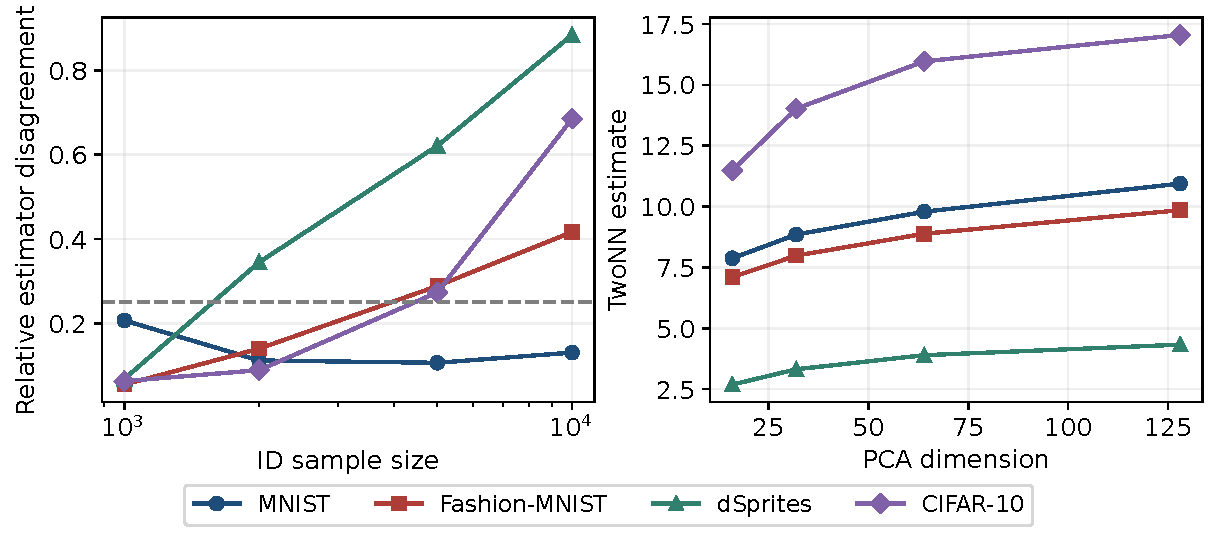
\includegraphics[width=\textwidth]{results/figures/MAKE51/id.pdf}
\caption{Left: $|d_{\rm TwoNN}-d_{\rm MLE}|/d_{\rm TwoNN}$ on raw
inputs as estimation sample size changes; dashed line is 0.25. Right:
TwoNN after PCA preprocessing. PCA rank, sample size and representation
are distinct interventions; AE results are in Table~\ref{tab:id}.}
\label{fig:id}
\end{figure}

\subsection{Dependence on Regularisation and Quality Context}\label{sec:beta}
Define the reported range for method $a$ and dataset $d$ by
\begin{equation}
 S_{a,d}=\max_{\beta\in\mathcal B}\bar m_{a,d}(\beta)
         -\min_{\beta\in\mathcal B}\bar m_{a,d}(\beta),\qquad
 \bar m_{a,d}(\beta)=\frac15\sum_{s=1}^{5}m_{a,d,s}(\beta),
 \quad\mathcal B=\{0.25,0.5,1,2,4\}.
 \label{eq:span}
\end{equation}
This is the range of seed means of raw returned dimensions, not the mean
of within-seed ranges. For the FONDUE-VAR row all five outputs are
defined at each setting, including any raw zero. It is a descriptive
range on the tested ladder, not a new parameter-free robustness index.

\begin{table}[H]
\caption{Range of seed-mean returned dimensions across $\beta\in\{0.25,0.5,1,2,4\}$. Pruning adaptations are restricted to the implementation audit. Fixed 32 is a design constant; fallback spans are not ID robustness. Gaussian likelihood except Bernoulli dSprites.}\label{tab:span}
\small
\setlength{\tabcolsep}{3.5pt}
\begin{tabular*}{\textwidth}{@{\extracolsep{\fill}}lcccc@{}}
\toprule
Method & MNIST & Fashion & dSprites & CIFAR-10 \\
\midrule
Grid (MSE) & 14.8 & 20.8 & 40.0 & 91.2 \\
Coarse search & 33.6 & 37.2 & 0.0 & 214.4 \\
Fixed 32 & 0.0 & 0.0 & 0.0 & 0.0 \\
FONDUE & 3.8 & 0.8 & 0.8 & 8.8 \\
FONDUE-VAR (mixed kept) & 50.6 & 63.0 & 106.2 & 68.8 \\
Ascending + Q & 6.0 & 3.6 & 15.2 & 52.8 \\
FONDUE + Q & 3.6 & 1.6 & 28.0 & 44.8 \\
Legacy ID window & 6.0 & 37.2 & 0.0 & 214.4 \\
\bottomrule
\end{tabular*}
\end{table}


Ranges differ by method and dataset, with clear ordering reversals.
For example, ascending versus FONDUE+$Q$ ranges are 6.0 versus 3.6
on MNIST, but 15.2 versus 28.0 on dSprites. The legacy ID window's
CIFAR-10 range of 214.4 is inherited from fallback. A fixed dimension has zero range by design;
dSprites ID fallback has zero range because coarse search always returns
64. Neither demonstrates useful selection robustness. We do not average
ranges across differently scaled grids or assert a transferable ranking.

The ARD call did not vary its selection-stage weight and GECO varied an
anchor-derived constraint rather than $\beta$ directly. Both belong
to the implementation audit, not Figure~\ref{fig:beta}'s ordinary-VAE
regularisation comparison.

\begin{figure}[!htbp]
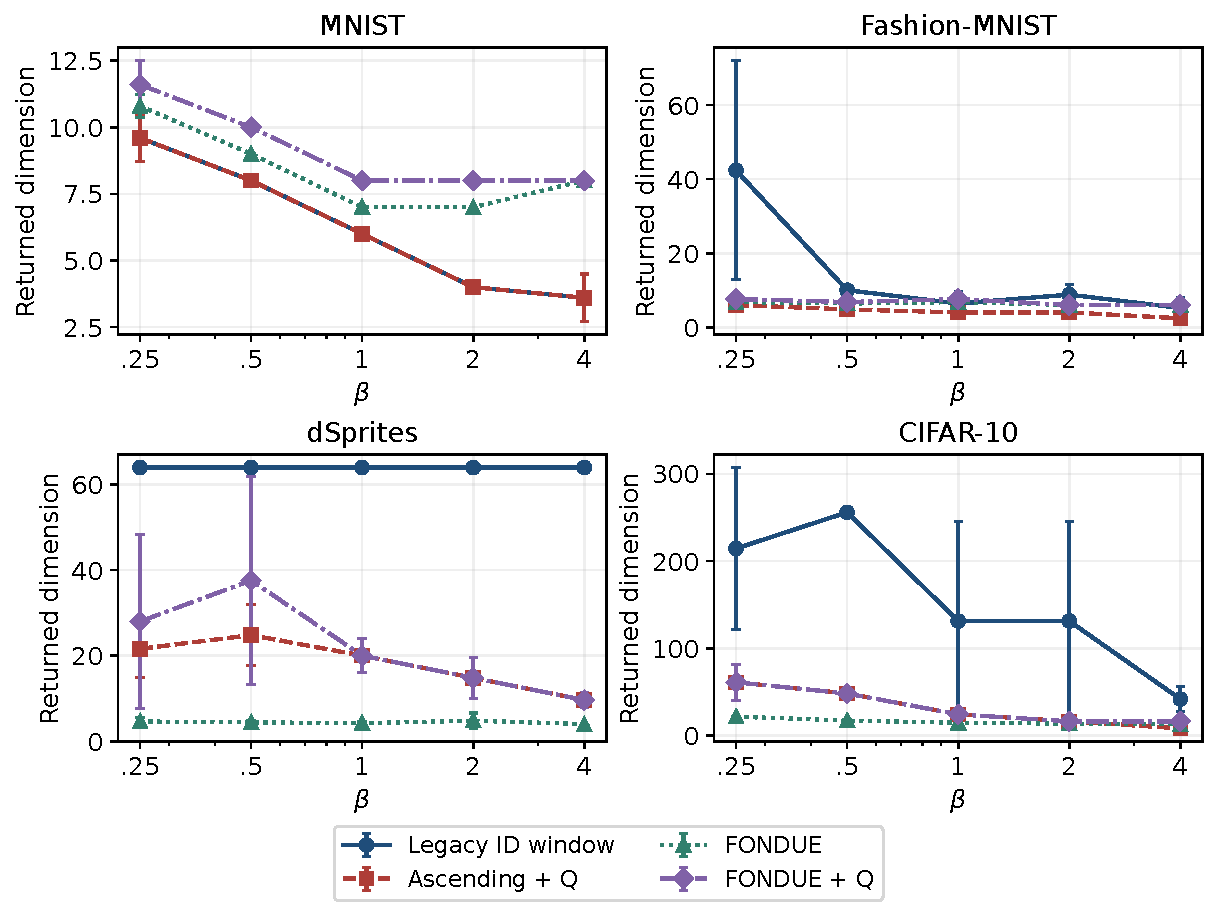
\includegraphics[width=\textwidth]{results/figures/MAKE51/beta.pdf}
\caption{Raw returned dimension across the five contexts, mean $\pm$ SD
over five candidate seeds. Gaussian likelihood except Bernoulli dSprites.
These ordinary VAE selectors change training $\beta$. The legacy ID
window falls back on
Fashion-MNIST, dSprites and CIFAR-10 throughout the ladder.}
\label{fig:beta}
\end{figure}

An AU-threshold intervention holds the checkpoint fixed and recomputes
Equation~\eqref{eq:au}. A quality-margin intervention instead changes
which cached models satisfy the target. Neither is the same as changing
training $\beta$. We report these readout/quality analyses separately
(Section~\ref{sec:au} and Appendix~\ref{app:sensitivity}). No sensitivity
claim is made for untested FONDUE stopping thresholds or ARD cumulative
relevance fractions.

\subsection{Learning Curves, Test Evaluation and Selection Criteria}
Figure~\ref{fig:selectedcurves} uses actual early-stopped cache records
selected by ascending-$Q$ at the primary setting, including MNIST width
six and CIFAR-10. Each run is shown only over its recorded epochs and
the proxy-selected checkpoint is marked. These cache records contain
validation curves but no epoch-wise train curve; no missing train
measurements are imputed. The separate new MNIST run supplies matched
train/validation curves for width six (Appendix~\ref{app:newmodels}).

\begin{figure}[!htbp]
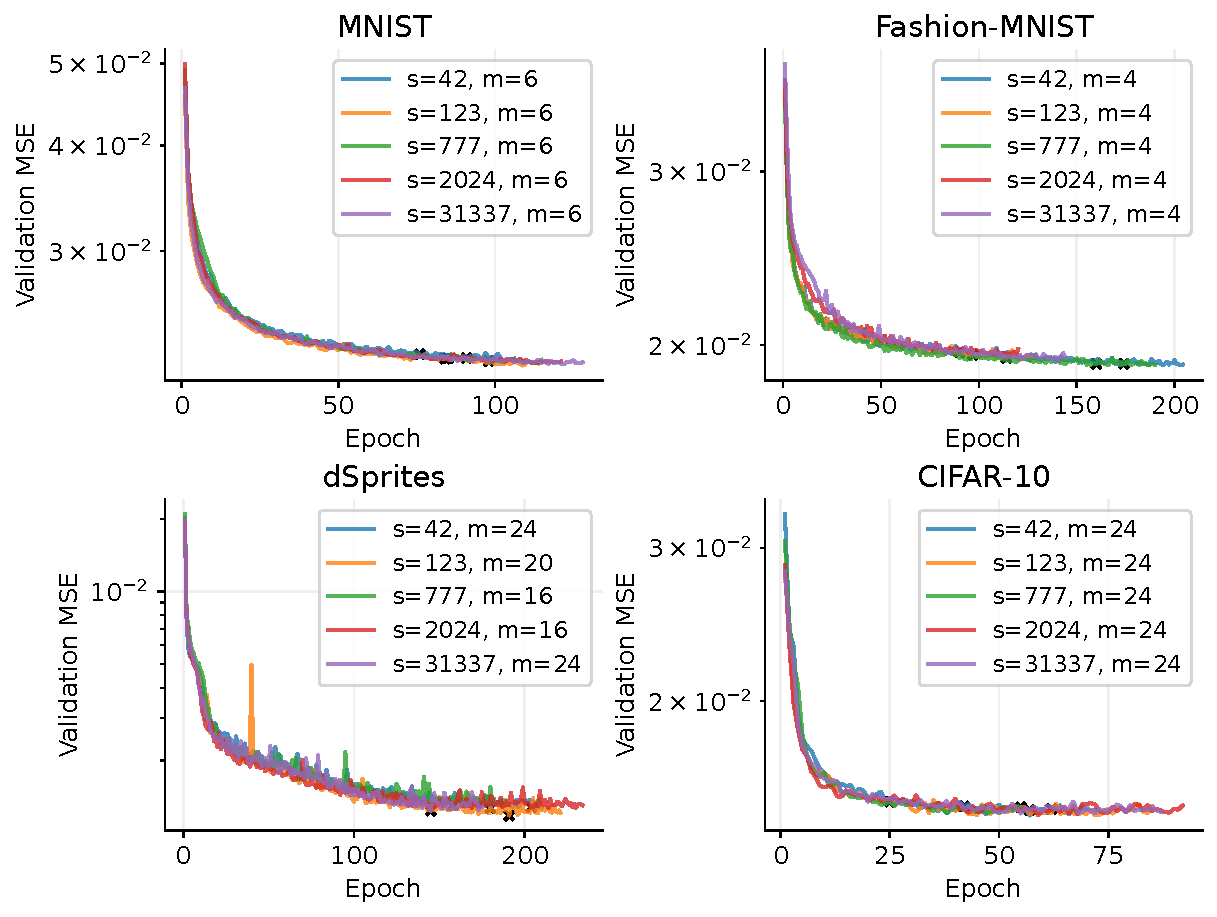
\includegraphics[width=\textwidth]{results/figures/MAKE51/selected_curves.pdf}
\caption{Actual selected-candidate validation MSE at $\beta=1$, five
seeds, Gaussian likelihood except Bernoulli dSprites. Widths are chosen
by ascending-$Q$; black crosses mark proxy-selected epochs. Curves end
at the recorded stopping time. These are not the fixed-300-epoch
diagnostic runs in Figure~\ref{fig:learning}.}
\label{fig:selectedcurves}
\end{figure}

The saved trajectory experiment supplies train/validation curves for
MNIST widths 12, 32 and 64 and dSprites widths 6, 16 and 32, with five
seeds each (Figure~\ref{fig:learning}). Training MSE is evaluated in
deterministic mode on a fixed 2000-example training subset sampled with
seed 20260919. Both train and validation improve, but validation error
remains higher. None of these 30 runs passes the stringent final
50-epoch plateau check; completing 300 epochs is not proof of convergence.
These curves cover representative settings, not all four datasets.

\begin{figure}[!htbp]
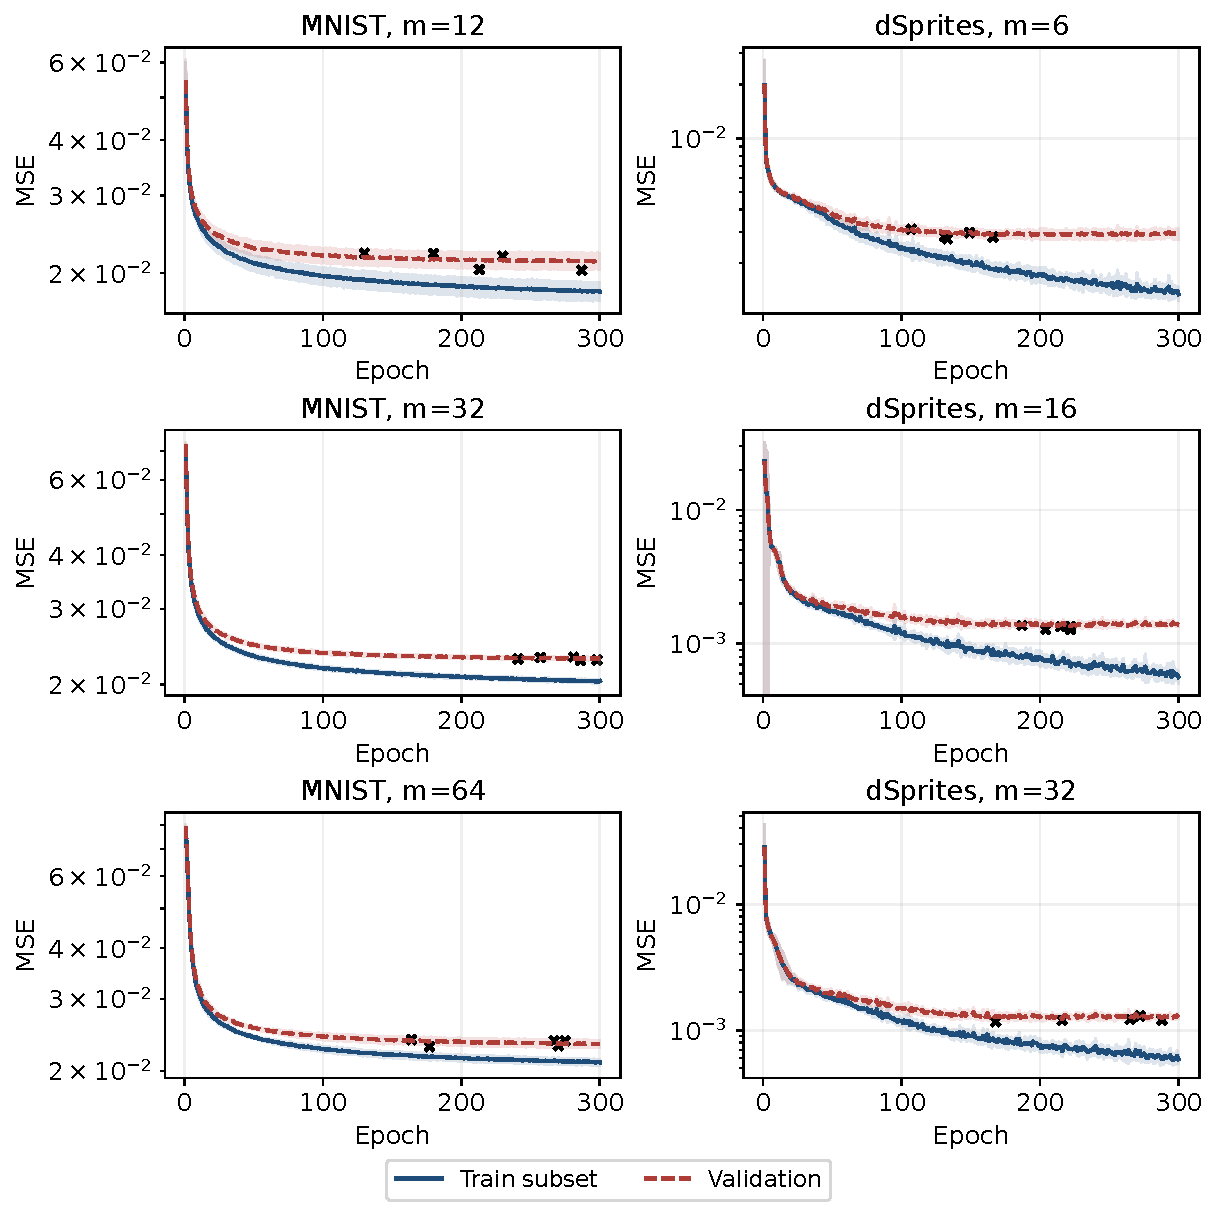
\includegraphics[width=\textwidth]{results/figures/MAKE51/learning.pdf}
\caption{Train and validation MSE, means with $\pm$1 SD bands over five
seeds. MNIST uses Gaussian and dSprites Bernoulli likelihood; $\beta=1$.
Black crosses mark each run's checkpoint selected by the validation
ELBO proxy. These diagnostic runs have no early stopping.}
\label{fig:learning}
\end{figure}

\begin{table}[H]
\caption{Selection-criterion comparison at $\beta=1$, five seeds; test MSE $\times10^3$ and probe test accuracy (\%). Probes use class labels (shape for dSprites); only Grid (probe) uses them for capacity selection. Time is the historical ledger including anchor completion, not the canonical replay price. Recorded probe time is charged to that selector. Other displayed probe accuracies are auxiliary evaluations with uncharged costs. Likelihoods follow Table~\ref{tab:data}.}\label{tab:selection}
\footnotesize
\setlength{\tabcolsep}{3.5pt}
\begin{tabular*}{\textwidth}{@{\extracolsep{\fill}}llcccc@{}}
\toprule
Dataset & Criterion & $m$ & Test MSE & Accuracy & Time (s) \\
\midrule
MNIST & Grid (MSE) & $12.8 \pm 6.4$ & $20.50 \pm 0.26$ & $89.4 \pm 0.9$ & $628 \pm 35$ \\
MNIST & Grid (ELBO proxy) & $10.0 \pm 2.0$ & $20.54 \pm 0.25$ & $89.3 \pm 0.7$ & $628 \pm 35$ \\
MNIST & Grid (probe) & $51.2 \pm 13.4$ & $23.01 \pm 0.55$ & $92.7 \pm 0.5$ & $696 \pm 36$ \\
Fashion-MNIST & Grid (MSE) & $22.8 \pm 15.6$ & $18.08 \pm 0.19$ & $75.5 \pm 2.6$ & $645 \pm 42$ \\
Fashion-MNIST & Grid (ELBO proxy) & $15.6 \pm 8.0$ & $18.12 \pm 0.27$ & $74.4 \pm 2.6$ & $645 \pm 42$ \\
Fashion-MNIST & Grid (probe) & $57.6 \pm 8.8$ & $18.99 \pm 0.46$ & $78.4 \pm 0.6$ & $750 \pm 40$ \\
dSprites & Grid (MSE) & $57.6 \pm 14.3$ & $1.15 \pm 0.01$ & $47.7 \pm 2.3$ & $2565 \pm 82$ \\
dSprites & Grid (ELBO proxy) & $57.6 \pm 14.3$ & $1.15 \pm 0.01$ & $47.7 \pm 2.3$ & $2565 \pm 82$ \\
dSprites & Grid (probe) & $64.0 \pm 0.0$ & $1.16 \pm 0.03$ & $49.8 \pm 3.0$ & $2589 \pm 84$ \\
CIFAR-10 & Grid (MSE) & $140.8 \pm 53.5$ & $14.07 \pm 0.04$ & $44.3 \pm 2.6$ & $428 \pm 16$ \\
CIFAR-10 & Grid (ELBO proxy) & $192.0 \pm 45.3$ & $14.11 \pm 0.08$ & $46.1 \pm 1.1$ & $428 \pm 16$ \\
CIFAR-10 & Grid (probe) & $256.0 \pm 0.0$ & $14.30 \pm 0.12$ & $47.3 \pm 1.0$ & $574 \pm 15$ \\
\bottomrule
\end{tabular*}
\end{table}


Table~\ref{tab:selection} provides the previously omitted grid choices
based on MSE, the ELBO proxy and a linear probe. Different objectives can
select different widths and reconstruction errors. Test probe accuracy
is an auxiliary supervised outcome; it does not measure unsupervised
reconstruction quality. This comparison retains the same splits and
cached candidates, with labelled validation selection explicitly stated.

The separate new MNIST comparison in Table~\ref{tab:mcselection}
evaluates an actual expected log likelihood with the fixed Monte Carlo
protocol in Section~\ref{sec:newvalidation}. It is not reconstructed
from cached MSE and KL. Validation MSE selects width 12, the proxy selects 12, and Monte Carlo ELBO selects 12. Agreement in this run does not make the proxy an ELBO estimator.
The complete grid scores, MC errors and selected epochs appear in
Appendix~\ref{app:newmodels}. One new training seed does not establish
a dataset-level advantage of any criterion. The additional four-dataset
pruning records do not extend this capacity-selection ELBO comparison,
for the evaluation-code reasons in Section~\ref{sec:gpuvalidation}.

\begin{table}[H]
\caption{New MNIST seed-42 capacity selection at $\beta=1$, Gaussian variance $1/2$. All criteria choose among the same twelve proxy-selected checkpoints. MSE is multiplied by $10^3$; ELBO is mean nats/example and its $\pm$ value is Monte Carlo SE ($K=32$), not a training-seed SD. Test is evaluated after validation choices are frozen.}\label{tab:mcselection}
\small
\setlength{\tabcolsep}{3pt}
\begin{tabular*}{\textwidth}{@{\extracolsep{\fill}}lcccc@{}}
\toprule
Criterion & Width & Val. MSE & Test MSE & MC ELBO $\pm$ MC SE \\
\midrule
MSE & 12 & 20.98 & 20.43 & $-478.067 \pm 0.012$ \\
ELBO proxy & 12 & 20.98 & 20.43 & $-478.067 \pm 0.012$ \\
MC ELBO & 12 & 20.98 & 20.43 & $-478.067 \pm 0.012$ \\
\bottomrule\end{tabular*}
\end{table}


\subsection{Activity Readout: Trajectories, Thresholds and Prediction}\label{sec:au}
Figure~\ref{fig:readouts} and Table~\ref{tab:readouts} compare the two
counts on identical checkpoints. At MNIST width 64, epoch-five variable
types give $9.8\pm3.8$ and AU gives $49.4\pm8.1$; at epoch 300 both
give $6.4\pm0.5$. This example distinguishes mean agreement from
between-seed variability. The table also reports within-run changes from
50 to 300 epochs. Their magnitude depends on the condition, so no
general stability superiority is inferred from the final agreement.

\begin{table}[H]
\caption{Variable-type count $V$ (active plus mixed) and AU count $A$, five seeds, $\beta=1$, Gaussian MNIST and Bernoulli dSprites. Mean $\pm$ SD quantify between-seed variation. The last column gives mean absolute within-run changes from epoch 50 to 300 for $V/A$, not a temporal variance.}\label{tab:readouts}
\footnotesize
\setlength{\tabcolsep}{3.5pt}
\begin{tabular*}{\textwidth}{@{\extracolsep{\fill}}lcccccc@{}}
\toprule
Dataset & $m$ & $V_5$ & $A_5$ & $V_{300}$ & $A_{300}$ & Change \\
\midrule
MNIST & 12 & $7.2 \pm 0.8$ & $8.0 \pm 1.6$ & $6.4 \pm 0.5$ & $6.4 \pm 0.5$ & 0.0/0.0 \\
MNIST & 32 & $8.2 \pm 1.5$ & $20.8 \pm 4.2$ & $6.0 \pm 0.0$ & $6.0 \pm 0.0$ & 0.0/0.0 \\
MNIST & 64 & $9.8 \pm 3.8$ & $49.4 \pm 8.1$ & $6.4 \pm 0.5$ & $6.4 \pm 0.5$ & 0.4/2.6 \\
dSprites & 6 & $6.0 \pm 0.0$ & $6.0 \pm 0.0$ & $6.0 \pm 0.0$ & $6.0 \pm 0.0$ & 0.0/0.0 \\
dSprites & 16 & $16.0 \pm 0.0$ & $16.0 \pm 0.0$ & $14.2 \pm 0.4$ & $13.4 \pm 0.5$ & 1.8/1.8 \\
dSprites & 32 & $32.0 \pm 0.0$ & $31.8 \pm 0.4$ & $14.2 \pm 1.1$ & $14.4 \pm 1.1$ & 12.4/4.2 \\
\bottomrule
\end{tabular*}
\end{table}


\begin{figure}[!htbp]
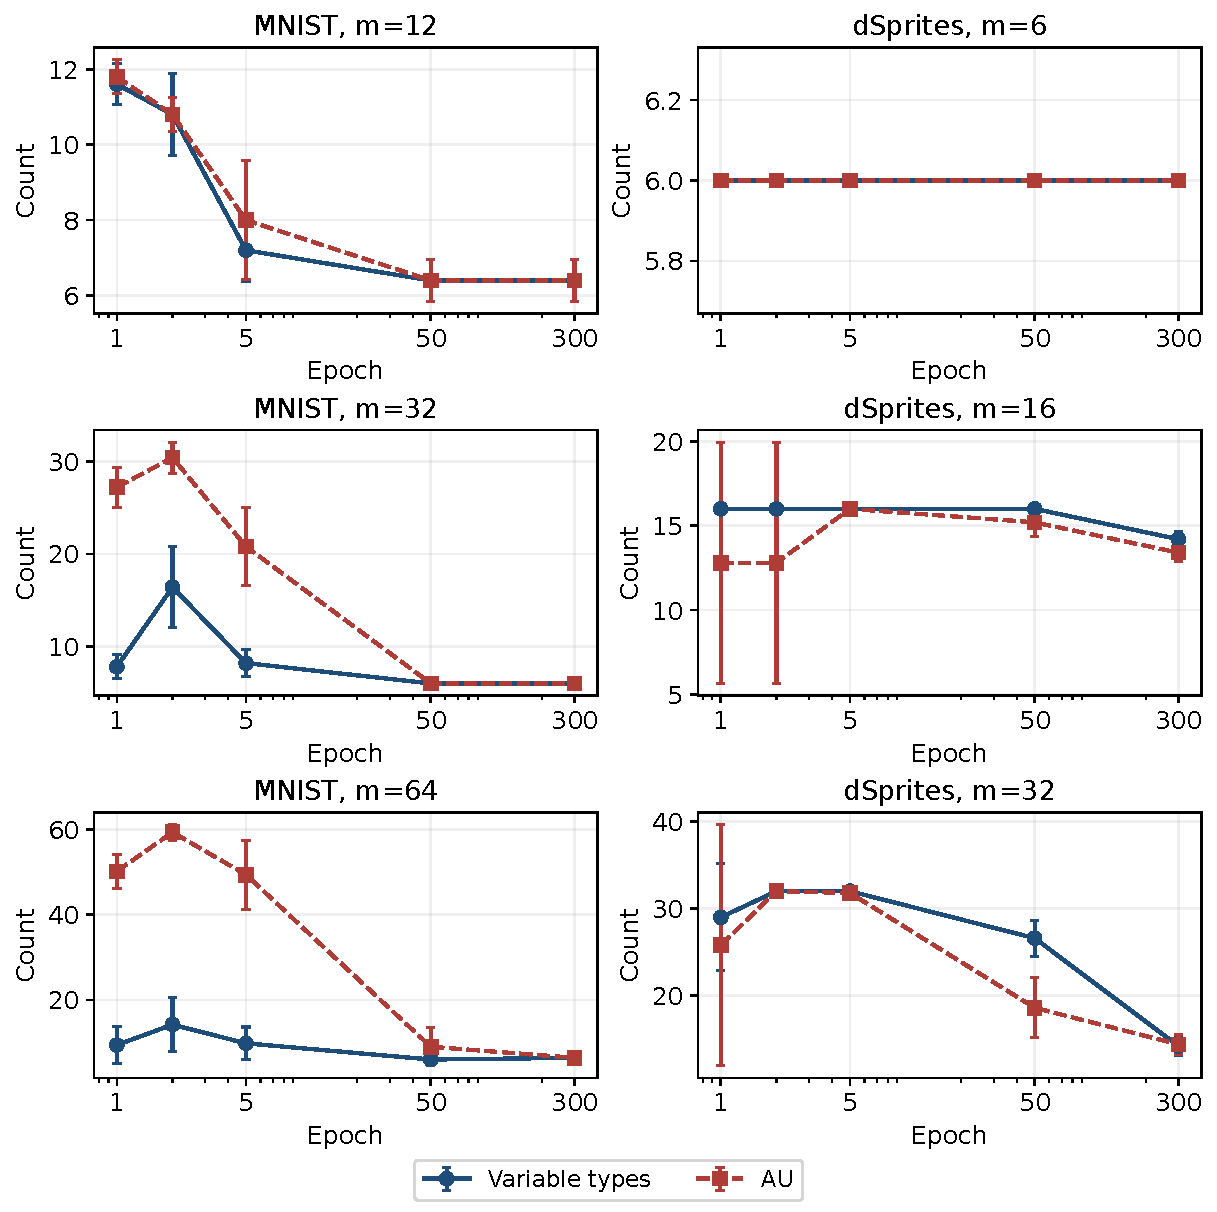
\includegraphics[width=\textwidth]{results/figures/MAKE51/readouts.pdf}
\caption{Variable-type count (active plus mixed) and AU from the same
checkpoints at epochs 1, 2, 5, 50 and 300; means and seed SDs, with lines
connecting the observed checkpoints only. $\beta=1$, Gaussian MNIST and
Bernoulli dSprites. Constant full-capacity counts are not evidence of
diagnostic stability.}
\label{fig:readouts}
\end{figure}

The threshold-only comparison in Figure~\ref{fig:delta} uses fixed
$\beta=1$ checkpoints. On CIFAR-10, $\delta=0.001$ counts every
coordinate at every tested grid width, whereas $\delta=0.1$ counts
far fewer at large widths. The inference ``no unused coordinates''
therefore depends on this threshold. Normalising the threshold changes
the diagnostic definition; it does not establish a dimension estimate.

\begin{figure}[!htbp]
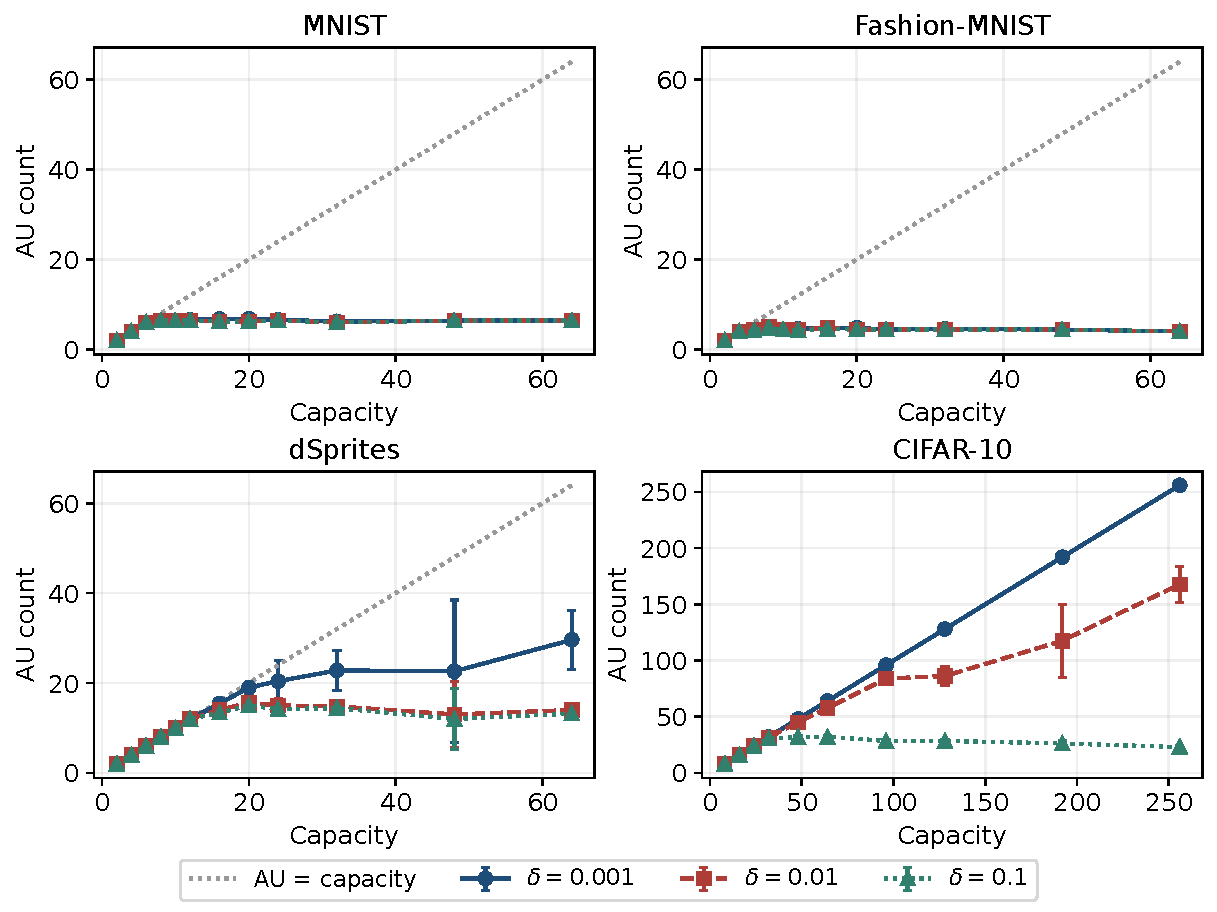
\includegraphics[width=\textwidth]{results/figures/MAKE51/delta.pdf}
\caption{AU under three thresholds on the same $\beta=1$ candidates;
mean $\pm$ seed SD. Gaussian likelihood except Bernoulli dSprites.
The diagonal is capacity. This is a readout-threshold intervention,
unlike the training/context intervention in Figure~\ref{fig:beta}.}
\label{fig:delta}
\end{figure}

The predictive task asks whether the next smaller grid candidate meets
the same seed's quality target. Each row is one validation-selected
checkpoint at a nonminimal grid width. Baseline features are validation
MSE, KL, the ELBO proxy, width, width/input-ID ratio, and the slope of
validation MSE over the last 20 recorded epochs. The three added AU
features are AU, AU/width and AU/input-ID. Standardisation is fitted
only on development rows. An $L_2$ logistic predictor is fitted on
MNIST (55 rows), with $C=10$ chosen on a three-seed/two-seed
development split. Evaluation uses dSprites (55 rows), Fashion-MNIST
(55) and CIFAR-10 (45), each with five seeds. The configured
MNIST-CNN predictive condition was not executed.

The development split uses seeds 42, 123 and 777 for the inner fit and
2024 and 31337 for selecting $C$, then refits on all five. Predictors use
up to 5000 iterations. Each evaluation dataset--seed block is scored
over its complete set of nonminimal grid widths; checkpoint rows are
not resampled as independent observations.

The original internally specified analysis reported an AU-minus-baseline
AUROC improvement of $+0.108$, with a 2000-replicate seed-record bootstrap
95\% interval $[+0.059,+0.157]$. A subsequently added control used
three independent standard-normal features and one noise realisation
(generator seed 7); its separately reported improvement was $+0.098$
with interval $[-0.025,+0.227]$. Overlap of these intervals does not test
their difference or establish equivalence. These archived values are
retained as the original analysis, not as a validated positive finding:
its AUROC calculation used probabilities that can saturate numerically
under the shift between datasets.

\begin{table}[H]
\caption{Retrospective paired AU comparison at $\beta=1$, using logistic decision scores to avoid saturated-probability ties. Values are means of five seed-specific AUROCs, each evaluated over all nonminimal capacities in that seed. Random features are three standard-normal columns with generator seed 7. All methods use the same rows and labels.}\label{tab:au}
\footnotesize
\setlength{\tabcolsep}{3.5pt}
\begin{tabular*}{\textwidth}{@{\extracolsep{\fill}}lccccc@{}}
\toprule
Evaluation condition & Rows & Base & Base + AU & Base + random & AU $-$ random \\
\midrule
dSprites & 55 & 0.950 & 0.858 & 0.898 & -0.041 \\
Fashion-MNIST & 55 & 0.980 & 1.000 & 0.880 & +0.120 \\
CIFAR-10 & 45 & 1.000 & 1.000 & 1.000 & +0.000 \\
\bottomrule
\end{tabular*}
\end{table}


Baseline AUROC is already 0.950, 0.980 and 1.000 on dSprites,
Fashion-MNIST and CIFAR-10, respectively. In particular, CIFAR-10 has
no upward AUROC headroom. The result concerns additional value on this
specific, near-ceiling prediction task, not the information content of
AU in general.

For this revision we reconstruct both predictors at explicitly fixed
$\beta=1$, restrict rows to the declared grid, and compute AUROC from
logistic decision scores. The original cache-reading routine did not
filter $\beta$ or restrict the grid, so rerunning it after cache expansion
would also be ambiguous. Decision scores preserve ranks that are lost
when sigmoid probabilities round to exactly one. Saturation counts
appear in Appendix~\ref{app:sensitivity}. This is a corrected retrospective
analysis, not an exact replay of archived probabilities. The
AU-minus-baseline difference is now $-0.024$, with interval
$[-0.102,+0.027]$. We also compare AU and random
predictors on the same dataset--seed blocks.
The paired mean difference is $+0.026$, with a retrospective
hierarchical-bootstrap 95\% interval $[-0.040,+0.133]$ (2000
replicates). Each replicate resamples the three evaluation datasets and
then the five seed blocks within each selected dataset; all capacities
and both predictors remain paired within a block. Models are held fixed,
so this interval does not cover development-model fitting uncertainty.
Only three evaluation datasets are available, limiting precision of
across-condition inference. A secondary analysis averages the comparator
over 100 noise realisations (seeds 0--99), giving a paired difference
$-0.007$ and interval $[-0.064,+0.039]$ under the
same resampling. Neither analysis establishes an AU-specific benefit in
these evaluation conditions. We do not claim that AU has no information,
that the predictors are equivalent, or that lack of significance proves
insufficient power.

\subsection{Implementation Audit and Degenerate Outputs}
Historical loss-scaling corrections are documented in
Appendix~\ref{app:scaling}. Current image comparisons use the corrected
sum-over-latents convention.

A further ARM-specific implementation check concerns averaging order.
The supplied linear-loss test compares the per-example antithetic
estimator with its analytic gradient; averaging losses before forming
their correlation with the gate samples removes the required pairing.
The additional training code uses per-example losses. This component
correction does not imply all constraints are satisfied: endpoint
counts are shown in Table~\ref{tab:armnew}. It is distinct from the
historical loss-scaling and ARD relevance-normalisation audits.

FONDUE-VAR's active-only setting returning zero is a separate phenomenon,
not a third sum/mean defect. At MNIST's one-epoch setting it returns zero
on all five trials; no final VAE exists for these outputs.
Table~\ref{tab:var} shows both settings and their quality/validity counts.

\begin{table}[H]
\caption{FONDUE-VAR at $\beta=1$: both keep-mixed settings, valid-model and quality counts, test MSE $\times10^3$, and recorded training time. Raw zero outputs remain in the dimension summary; nonexistent models have no MSE. Five seeds; likelihoods follow Table~\ref{tab:data}.}\label{tab:var}
\footnotesize
\setlength{\tabcolsep}{3.5pt}
\begin{tabular*}{\textwidth}{@{\extracolsep{\fill}}lcccccc@{}}
\toprule
Dataset & Mixed kept & Raw $m$ & Valid & $Q$ & Test MSE & Time (s) \\
\midrule
MNIST & yes & $9.8 \pm 8.5$ & 5/5 & 5/5 & $22.53 \pm 0.89$ & $113 \pm 22$ \\
MNIST & no & $0.0 \pm 0.0$ & 0/5 & 0/5 & --- & $63 \pm 10$ \\
Fashion-MNIST & yes & $14.4 \pm 3.8$ & 5/5 & 5/5 & $18.96 \pm 0.39$ & $91 \pm 11$ \\
Fashion-MNIST & no & $2.0 \pm 0.0$ & 5/5 & 0/5 & $25.27 \pm 0.06$ & $120 \pm 18$ \\
dSprites & yes & $26.0 \pm 49.5$ & 4/5 & 1/5 & $9.53 \pm 9.62$ & $412 \pm 118$ \\
dSprites & no & $1.2 \pm 1.6$ & 2/5 & 0/5 & $7.71 \pm 0.02$ & $278 \pm 49$ \\
CIFAR-10 & yes & $34.2 \pm 1.3$ & 5/5 & 5/5 & $14.40 \pm 0.15$ & $103 \pm 13$ \\
CIFAR-10 & no & $3.2 \pm 0.8$ & 5/5 & 0/5 & $31.65 \pm 2.68$ & $96 \pm 13$ \\
\bottomrule
\end{tabular*}
\end{table}


\section{Discussion}\label{sec:discussion}
The controlled start-width ablation changes the interpretation of the
ID-local result. Its 100/100 minimum-width agreement is reproduced by
an ID-gated midpoint with the same fallback. Within the 25 accepted-ID
conditions, the ID start requires more candidates without changing the
answer. The bank-free midpoint's two errors occur where the ID policies
use ascending fallback. Consequently, this evidence does not establish
an advantage of the ID-derived start. Reliability-gated search and an
informative geometric starting width are distinct hypotheses.

The target includes the largest-width anchor, so quality attainment by
an exhaustive upward path is guaranteed within the stored grid.
Minimality and cost remain substantive outcomes. The factorial analysis
finds nonminimal outputs in 155 of 10,000 settings; the default agreement
is not a universal local-search guarantee. Shared reference banks, one
split, retrospective policy design and four datasets limit inference.
An independent reference-bank replication remains open. Acquisition
and reuse costs also answer different deployment questions.

Regularisation ranges and AU-threshold responses measure different
interventions. Some dimension ranges reflect fallback, grid scale or a
changing quality target. A constant output may be fixed by design or by
an unvaried implementation argument. The paired predictive comparison
does not establish an AU-specific advantage over matched random-feature
controls on its near-ceiling task. This limits the role of AU here to
a diagnostic of coordinate use under a stated threshold.

The native-pruning comparison shows why a selected count and the
reconstruction of a retained-axis model must be evaluated separately.
The local sample-centred ARD variant preserves mean MSE closely under
masking on MNIST and Fashion-MNIST, whereas dSprites deteriorates
substantially and only partly recovers with decoder adaptation.
Its full model already misses $Q$, which prevents presenting any of
the four dSprites conditions as successful target-preserving compression.
Masking tests an inference rule in the original network, not a measured
reduction in parameters, memory or latency. The fixed adaptation
budget also adds training and uses the previously reserved prior-update
pool. No unmasked 30-epoch adaptation control was run, so its improvement
cannot be assigned specifically to compensating for the mask.

These results extend the native-quality evidence to three seeds on each
dataset while retaining local training choices. Exact Jacobians remove
finite-step approximation, not uncertainty in the sampled relevance
score or the trained representation. The Gaussian KL approximation is
shared with the ARD source; the sample-centred variance update remains
a sensitivity variant, not a necessary correction of the source's
zero-centre setting. This variant's results cannot be generalised to
all ARD configurations or treated as an exact source-method benchmark.

The additional four-dataset ELBO fields do not compute the expected
likelihood and native prior KL needed for the claimed quantity. Valid
MC ELBO capacity-selection evidence remains one MNIST seed and
proxy-selected checkpoints. Likewise, new pruning curves do not recover
missing historical ordinary-VAE curves. Full source-algorithm reproduction,
independent-bank validation, complete end-to-end timing and clean synthetic
held-out evaluation remain uncompleted. The synthetic diagnostics
(Appendix~\ref{app:synthetic}) describe scale and coordinate effects;
they do not show that topology determines active-axis counts.

\section{Conclusions}\label{sec:conclusion}
We evaluated intrinsic-dimension-guided VAE bottleneck selection and
active-unit diagnostics under explicit quality and cost definitions.
Holding reliability checks, fallback and reference costs fixed, ID is
accepted only for the 25 MNIST conditions. ID-derived and gated
midpoint starts then select the same widths with 8.84 and 5.84 requests
on average; the other 75 conditions use the same ascending fallback.
Local-search minimality also depends on reliability and coefficient
settings. Additional pruning experiments distinguish native quality,
transferred-width quality and training constraints. In the local
sample-centred ARD variant, selected-axis masking changes reconstruction
little on two datasets but raises dSprites MSE by 126.3\%; decoder
adaptation only partly recovers this loss, and all four dSprites
conditions miss $Q$. AU does not establish additional predictive value
on the present near-ceiling task. The contribution is a bounded
evaluation of ID guidance and latent diagnostics; it establishes
neither a general efficiency advantage nor guaranteed pruning quality.

\authorcontributions{Conceptualization, C.O., M.D. and K.J.; methodology,
C.O. and K.J.; software, C.O. and M.D.; validation, C.O., M.D. and K.J.;
formal analysis, C.O. and K.J.; investigation, C.O., M.D. and K.J.;
writing---original draft preparation, C.O. and K.J.; writing---review and
editing, C.O., M.D. and K.J.; supervision and project administration, K.J.}
\funding{This research was funded by JSPS KAKENHI Grant Numbers
JP24K15115 and JP26K14984, by the Tokyo City University Priority Research
[Intelligent Technology Optimization Research Unit: ORBIT], by a
Cooperative Research Project of the Research Institute of Electrical
Communication (RIEC), Tohoku University, and by a Research Grant from the
Telecommunications Advancement Foundation (TAF).}
\institutionalreview{Not applicable.}
\informedconsent{Not applicable.}
\dataavailability{The image datasets are publicly available from their
cited sources. The accompanying reviewer supplement
\texttt{MAKE53\_reproducibility.zip} contains configuration, historical
and additional result records, analysis and training code, split indices,
figures, separate MNIST validation checkpoints and a SHA-256 manifest.
Extract the archive and follow its \texttt{README.md};
Appendix~\ref{app:inventory} maps its contents. Historical MAKE49 and
additional MAKE52 pruning checkpoints are unavailable. The archive is
supplied with this revision; it is not a public data deposit and has no DOI.}
\acknowledgments{Generative-AI assistance was used for experimental-code
drafting and refactoring and English-language editing in the earlier
manuscript preparation. OpenAI Codex assisted with the present record
audit, reaggregation, model-validation analysis, figure preparation
and manuscript revision.
Responsibility for the scientific content rests with the authors.}
\conflictsofinterest{The authors declare no conflicts of interest.}

\appendixtitles{yes}
\appendixstart
\appendix
\section{Quality Targets and Outcome Accounting}\label{app:targets}
\begin{table}[H]
\caption{Quality anchors and targets, in units of $10^{-3}$ MSE, mean $\pm$ SD over five seeds. Each decision uses its own seed-specific target, not the displayed mean. The relative margin is 10\%; the absolute floor is inactive. Gaussian likelihood except Bernoulli dSprites.}\label{tab:anchors}
\small
\setlength{\tabcolsep}{3.5pt}
\begin{tabular*}{\textwidth}{@{\extracolsep{\fill}}lccc@{}}
\toprule
Dataset & $\beta$ & Anchor MSE & Target $T_{D,s}$ \\
\midrule
MNIST & 0.25 & $15.843 \pm 0.562$ & $17.428 \pm 0.618$ \\
MNIST & 0.5 & $19.202 \pm 0.497$ & $21.122 \pm 0.546$ \\
MNIST & 1 & $23.712 \pm 0.532$ & $26.084 \pm 0.585$ \\
MNIST & 2 & $30.061 \pm 0.560$ & $33.068 \pm 0.617$ \\
MNIST & 4 & $38.977 \pm 0.673$ & $42.875 \pm 0.740$ \\
Fashion-MNIST & 0.25 & $15.591 \pm 0.678$ & $17.150 \pm 0.746$ \\
Fashion-MNIST & 0.5 & $17.408 \pm 0.513$ & $19.148 \pm 0.564$ \\
Fashion-MNIST & 1 & $19.679 \pm 0.162$ & $21.647 \pm 0.179$ \\
Fashion-MNIST & 2 & $22.416 \pm 0.527$ & $24.658 \pm 0.580$ \\
Fashion-MNIST & 4 & $25.967 \pm 0.587$ & $28.564 \pm 0.645$ \\
dSprites & 0.25 & $1.015 \pm 0.032$ & $1.117 \pm 0.036$ \\
dSprites & 0.5 & $1.040 \pm 0.032$ & $1.144 \pm 0.035$ \\
dSprites & 1 & $1.170 \pm 0.024$ & $1.287 \pm 0.026$ \\
dSprites & 2 & $1.453 \pm 0.038$ & $1.598 \pm 0.041$ \\
dSprites & 4 & $2.144 \pm 0.064$ & $2.358 \pm 0.070$ \\
CIFAR-10 & 0.25 & $9.407 \pm 0.610$ & $10.348 \pm 0.671$ \\
CIFAR-10 & 0.5 & $11.151 \pm 0.200$ & $12.266 \pm 0.220$ \\
CIFAR-10 & 1 & $14.064 \pm 0.108$ & $15.470 \pm 0.119$ \\
CIFAR-10 & 2 & $17.806 \pm 0.262$ & $19.587 \pm 0.288$ \\
CIFAR-10 & 4 & $22.399 \pm 0.286$ & $24.638 \pm 0.314$ \\
\bottomrule
\end{tabular*}
\end{table}


\subsection{Independent Outcome Counts}\label{app:outcomes}
The following tables separate the original combined state from flags and
final-model quality. A budget flag can coexist with ID fallback. The
pruning wrapper did not enforce the ordinary selector budget during
training, so its zero budget-flag count is not evidence of equal budget
control. All valid returned models, including those from budget-exceeded
trials, contribute to the primary means. Degenerate outputs contribute
to raw-count and cost summaries but not to MSE.
\begin{table}[H]
\caption{Outcome audit at $\beta=1$; all counts have denominator five. S: recorded success; I: ID unreliable; B: budget exceeded; D: degenerate; N: no compact alternative. FB is the fallback flag; budget, validation quality $Q$, and compression of the final VAE are independently recomputed or read from flags.}\label{tab:outcomes0}
\footnotesize
\setlength{\tabcolsep}{3.5pt}
\begin{tabular*}{\textwidth}{@{\extracolsep{\fill}}llccccc@{}}
\toprule
Dataset & Method & State & FB & Budget & $Q$ & Compact \\
\midrule
MNIST & Grid (MSE) & S5 & 0 & 0 & 5 & 5 \\
MNIST & FONDUE & S5 & 0 & 0 & 5 & 5 \\
MNIST & FONDUE + Q & S5 & 0 & 0 & 5 & 5 \\
MNIST & GECO adaptation & S5 & 0 & 0 & 5 & 5 \\
MNIST & ARD adaptation & S5 & 0 & 0 & 5 & 5 \\
MNIST & Ascending + Q & S5 & 0 & 0 & 5 & 5 \\
MNIST & Legacy ID window & S5 & 0 & 0 & 5 & 5 \\
MNIST & FONDUE-VAR (mixed kept) & S5 & 0 & 0 & 5 & 5 \\
MNIST & FONDUE-VAR (active only) & D5 & 0 & 0 & 0 & 0 \\
Fashion-MNIST & Grid (MSE) & S5 & 0 & 0 & 5 & 5 \\
Fashion-MNIST & FONDUE & S5 & 0 & 0 & 5 & 5 \\
Fashion-MNIST & FONDUE + Q & S5 & 0 & 0 & 5 & 5 \\
Fashion-MNIST & GECO adaptation & S5 & 0 & 0 & 5 & 5 \\
Fashion-MNIST & ARD adaptation & S5 & 0 & 0 & 4 & 5 \\
Fashion-MNIST & Ascending + Q & S5 & 0 & 0 & 5 & 5 \\
Fashion-MNIST & Legacy ID window & I5 & 5 & 0 & 5 & 5 \\
Fashion-MNIST & FONDUE-VAR (mixed kept) & S5 & 0 & 0 & 5 & 5 \\
Fashion-MNIST & FONDUE-VAR (active only) & S5 & 0 & 0 & 0 & 5 \\
\bottomrule
\end{tabular*}
\end{table}

\begin{table}[H]
\caption{Outcome audit at $\beta=1$; all counts have denominator five. S: recorded success; I: ID unreliable; B: budget exceeded; D: degenerate; N: no compact alternative. FB is the fallback flag; budget, validation quality $Q$, and compression of the final VAE are independently recomputed or read from flags.}\label{tab:outcomes1}
\footnotesize
\setlength{\tabcolsep}{3.5pt}
\begin{tabular*}{\textwidth}{@{\extracolsep{\fill}}llccccc@{}}
\toprule
Dataset & Method & State & FB & Budget & $Q$ & Compact \\
\midrule
dSprites & Grid (MSE) & S5 & 0 & 0 & 5 & 1 \\
dSprites & FONDUE & S5 & 0 & 0 & 0 & 5 \\
dSprites & FONDUE + Q & B1, S4 & 0 & 1 & 5 & 5 \\
dSprites & GECO adaptation & S5 & 0 & 0 & 5 & 0 \\
dSprites & ARD adaptation & S5 & 0 & 0 & 0 & 5 \\
dSprites & Ascending + Q & S5 & 0 & 0 & 5 & 5 \\
dSprites & Legacy ID window & I5 & 5 & 0 & 5 & 0 \\
dSprites & FONDUE-VAR (mixed kept) & D1, S4 & 0 & 0 & 1 & 3 \\
dSprites & FONDUE-VAR (active only) & D3, S2 & 0 & 0 & 0 & 2 \\
CIFAR-10 & Grid (MSE) & S5 & 0 & 0 & 5 & 5 \\
CIFAR-10 & FONDUE & S5 & 0 & 0 & 0 & 5 \\
CIFAR-10 & FONDUE + Q & S5 & 0 & 0 & 5 & 5 \\
CIFAR-10 & GECO adaptation & S5 & 0 & 0 & 2 & 5 \\
CIFAR-10 & ARD adaptation & S5 & 0 & 0 & 0 & 5 \\
CIFAR-10 & Ascending + Q & S5 & 0 & 0 & 5 & 5 \\
CIFAR-10 & Legacy ID window & I5 & 5 & 0 & 5 & 3 \\
CIFAR-10 & FONDUE-VAR (mixed kept) & S5 & 0 & 0 & 5 & 5 \\
CIFAR-10 & FONDUE-VAR (active only) & S5 & 0 & 0 & 0 & 5 \\
\bottomrule
\end{tabular*}
\end{table}


\section{Search Sensitivity and Timing Lineage}\label{app:search}
These tables use the retrospective policy in Algorithm~\ref{alg:replay}.
They do not redefine the original experiments.
\begin{table}[H]
\caption{Coefficient sensitivity for ID-local replay at $\beta=1$, with $R\le0.15$ and $A\le0.25$. All five coefficients are reported; rejected datasets use the same ascending fallback. Five seeds; likelihoods as in Table~\ref{tab:data}.}\label{tab:coefficient}
\small
\setlength{\tabcolsep}{3pt}
\begin{tabular*}{\textwidth}{@{\extracolsep{\fill}}lcccccc@{}}
\toprule
Dataset & $c$ & Width & $Q$ & Exact & Calls & Cold cost (s) \\
\midrule
MNIST & 1 & $6.0 \pm 0.0$ & 5/5 & 5/5 & 6.0 & 487 \\
MNIST & 1.5 & $6.0 \pm 0.0$ & 5/5 & 5/5 & 8.0 & 584 \\
MNIST & 2 & $6.0 \pm 0.0$ & 5/5 & 5/5 & 9.0 & 636 \\
MNIST & 3 & $6.0 \pm 0.0$ & 5/5 & 5/5 & 11.0 & 743 \\
MNIST & 4 & $6.0 \pm 0.0$ & 5/5 & 5/5 & 11.0 & 743 \\
Fashion-MNIST & 1 & $4.0 \pm 0.0$ & 5/5 & 5/5 & 3.0 & 416 \\
Fashion-MNIST & 1.5 & $4.0 \pm 0.0$ & 5/5 & 5/5 & 3.0 & 416 \\
Fashion-MNIST & 2 & $4.0 \pm 0.0$ & 5/5 & 5/5 & 3.0 & 416 \\
Fashion-MNIST & 3 & $4.0 \pm 0.0$ & 5/5 & 5/5 & 3.0 & 416 \\
Fashion-MNIST & 4 & $4.0 \pm 0.0$ & 5/5 & 5/5 & 3.0 & 416 \\
dSprites & 1 & $20.0 \pm 4.0$ & 5/5 & 5/5 & 9.0 & 2092 \\
dSprites & 1.5 & $20.0 \pm 4.0$ & 5/5 & 5/5 & 9.0 & 2092 \\
dSprites & 2 & $20.0 \pm 4.0$ & 5/5 & 5/5 & 9.0 & 2092 \\
dSprites & 3 & $20.0 \pm 4.0$ & 5/5 & 5/5 & 9.0 & 2092 \\
dSprites & 4 & $20.0 \pm 4.0$ & 5/5 & 5/5 & 9.0 & 2092 \\
CIFAR-10 & 1 & $24.0 \pm 0.0$ & 5/5 & 5/5 & 4.0 & 498 \\
CIFAR-10 & 1.5 & $24.0 \pm 0.0$ & 5/5 & 5/5 & 4.0 & 498 \\
CIFAR-10 & 2 & $24.0 \pm 0.0$ & 5/5 & 5/5 & 4.0 & 498 \\
CIFAR-10 & 3 & $24.0 \pm 0.0$ & 5/5 & 5/5 & 4.0 & 498 \\
CIFAR-10 & 4 & $24.0 \pm 0.0$ & 5/5 & 5/5 & 4.0 & 498 \\
\bottomrule\end{tabular*}
\end{table}

\begin{table}[H]
\caption{Reliability-threshold sensitivity at $\beta=1$, $c=2$. ID: local ID start; FB: ascending fallback. Extreme tolerances are stress conditions, not recommended thresholds. Each result uses five seeds and the same reference bank. The full factorial analysis is supplied in the supplement.}\label{tab:reliability}
\small
\setlength{\tabcolsep}{3pt}
\begin{tabular*}{\textwidth}{@{\extracolsep{\fill}}llccccc@{}}
\toprule
$R_{\max}/A_{\max}$ & Dataset & Use & Mean width & $Q$ & Exact & Calls \\
\midrule
0.1/0.25 & MNIST & FB & 6.0 & 5/5 & 5/5 & 4.0 \\
0.1/0.25 & Fashion-MNIST & FB & 4.0 & 5/5 & 5/5 & 3.0 \\
0.1/0.25 & dSprites & FB & 20.0 & 5/5 & 5/5 & 9.0 \\
0.1/0.25 & CIFAR-10 & FB & 24.0 & 5/5 & 5/5 & 4.0 \\
0.15/0.25 & MNIST & ID & 6.0 & 5/5 & 5/5 & 9.0 \\
0.15/0.25 & Fashion-MNIST & FB & 4.0 & 5/5 & 5/5 & 3.0 \\
0.15/0.25 & dSprites & FB & 20.0 & 5/5 & 5/5 & 9.0 \\
0.15/0.25 & CIFAR-10 & FB & 24.0 & 5/5 & 5/5 & 4.0 \\
0.25/0.25 & MNIST & ID & 6.0 & 5/5 & 5/5 & 9.0 \\
0.25/0.25 & Fashion-MNIST & FB & 4.0 & 5/5 & 5/5 & 3.0 \\
0.25/0.25 & dSprites & FB & 20.0 & 5/5 & 5/5 & 9.0 \\
0.25/0.25 & CIFAR-10 & FB & 24.0 & 5/5 & 5/5 & 4.0 \\
0.15/0.4 & MNIST & ID & 6.0 & 5/5 & 5/5 & 9.0 \\
0.15/0.4 & Fashion-MNIST & ID & 4.0 & 5/5 & 5/5 & 10.0 \\
0.15/0.4 & dSprites & FB & 20.0 & 5/5 & 5/5 & 9.0 \\
0.15/0.4 & CIFAR-10 & FB & 24.0 & 5/5 & 5/5 & 4.0 \\
0.15/0.85 & MNIST & ID & 6.0 & 5/5 & 5/5 & 9.0 \\
0.15/0.85 & Fashion-MNIST & ID & 4.0 & 5/5 & 5/5 & 10.0 \\
0.15/0.85 & dSprites & FB & 20.0 & 5/5 & 5/5 & 9.0 \\
0.15/0.85 & CIFAR-10 & ID & 24.0 & 5/5 & 5/5 & 4.0 \\
0.5/2 & MNIST & ID & 6.0 & 5/5 & 5/5 & 9.0 \\
0.5/2 & Fashion-MNIST & ID & 4.0 & 5/5 & 5/5 & 10.0 \\
0.5/2 & dSprites & ID & 20.0 & 5/5 & 5/5 & 6.0 \\
0.5/2 & CIFAR-10 & ID & 24.0 & 5/5 & 5/5 & 4.0 \\
\bottomrule\end{tabular*}
\end{table}


\subsection{Historical and Canonical Time Accounts}\label{app:timing}
Table~\ref{tab:cost} preserves the MAKE50 historical ledger, including
anchor completion where the original ledger omitted it. It is not the
price basis of the new replay. For example, MNIST's mean anchor prices
are 69.3~s in several early ledgers and 62.6~s in the later canonical
snapshot; width-six final-model prices are 39.9 and 37.6~s, respectively.
The logical conditions remain \texttt{e300|es1|b1} in these matches.
Identical metric summaries and requested conditions do not reveal why
two timing snapshots differ, nor prove bitwise model identity.
No unsupported cause such as different hardware or stopping settings
is assigned.

The supplementary \path{results/make51/cost_lineage.csv} gives each
dataset--method--weight--seed anchor/final role, complete key, original
trace key, file/record source, original duration, canonical duration and
available metric-identity check. Unretained off-grid candidates are
marked as unavailable. An absent historical anchor charge is distinguished
from a zero duration. The replay only requests retained grid candidates,
so every requested anchor and final model uses a single available
canonical metric/price record.
\begin{table}[H]
\caption{Anchor/final timing audit at $\beta=1$. Entries are method-role-seed records, not independent training runs. Different prices can be attached to the same logical cache key; full key, source and both durations are supplied in \texttt{cost\_lineage.csv}. Stored summary metrics do not establish checkpoint identity.}\label{tab:timing_audit}
\small
\setlength{\tabcolsep}{3pt}
\begin{tabular*}{\textwidth}{@{\extracolsep{\fill}}lccc@{}}
\toprule
Dataset & Matched entries & Different times & Max. difference (s) \\
\midrule
MNIST & 117 & 107 & 14.53 \\
Fashion-MNIST & 130 & 0 & 0.00 \\
dSprites & 119 & 109 & 0.42 \\
CIFAR-10 & 130 & 0 & 0.00 \\
\bottomrule\end{tabular*}
\end{table}

\begin{table}[H]
\caption{Historical MNIST training-time decomposition at $\beta=1$ (mean seconds, five seeds). The final model is charged once and removed from the other-candidate column. ID computation and post-training evaluation were not separately timed. FONDUE epoch calibration adds 4.14 s once per dataset--$\beta$ setting and is not included below.}\label{tab:cost}
\footnotesize
\setlength{\tabcolsep}{3.5pt}
\begin{tabular*}{\textwidth}{@{\extracolsep{\fill}}lrrrrr@{}}
\toprule
Method & Anchor & ID AEs & Other training & Final & Total \\
\midrule
Grid (MSE) & 69.3 & 0.0 & 502.0 & 56.2 & 627.5 \\
FONDUE & 62.6 & 0.0 & 1.4 & 39.9 & 103.9 \\
FONDUE + Q & 69.3 & 0.0 & 1.4 & 55.3 & 125.9 \\
GECO adaptation & 62.6 & 0.0 & 175.4 & 39.6 & 277.6 \\
ARD adaptation & 62.6 & 0.0 & 138.0 & 37.6 & 238.2 \\
Ascending + Q & 69.3 & 0.0 & 72.8 & 39.9 & 182.0 \\
Legacy ID window & 69.3 & 205.5 & 400.7 & 39.9 & 715.4 \\
\bottomrule
\end{tabular*}
\end{table}


\section{Coverage and Implementation Details}\label{app:coverage}
\begin{table}[H]
\caption{Executed coverage. Each image method row has five training
seeds at each listed context. Additional diagnostic experiments have
their own seed units.}
\label{tab:coverage}\small
\begin{tabularx}{\textwidth}{>{\raggedright\arraybackslash}p{0.34\textwidth}>{\raggedright\arraybackslash}p{0.19\textwidth}>{\raggedright\arraybackslash}X}\toprule
Experiment & Dataset coverage & Contexts / counts \\\midrule
Fourteen historical ordinary selectors/controls & All four image datasets & Five $\beta$ values; $14\times4\times5\times5=1400$ method records \\
Historical HC adaptation & All four & Five anchor-derived constraints; 100 records \\
Historical ARD adaptation & All four & Fixed selection-stage weight one; five repeated contexts, 100 records \\
ID-reference bank & All four & Three widths $\times$ three seeds each, shared across contexts \\
Train/validation and readout trajectories & MNIST: 12, 32, 64; dSprites: 6, 16, 32 & $\beta=1$, five seeds each; 30 runs \\
AU prediction & Develop: MNIST; evaluate: dSprites, Fashion-MNIST, CIFAR-10 & $\beta=1$; 55 development and 155 evaluation rows \\
Search replay and start-width ablation & All four & Seven policies, 700 rows; 10,000 coefficient/threshold settings \\
Separate MC ELBO capacity study & MNIST & One seed, 12 ordinary VAE widths \\
Additional ARM validation & All four & Three seeds, 12 runs; $\beta=1$ anchor \\
Additional exact-Jacobian ARD & All four & Three seeds, two variance-update centres; 24 runs \\
Native ARD masking and adaptation & All four & Three seeds; paired extension of sample-centred settings, 12 evaluations \\
Synthetic diagnostic & Swiss roll and torus & Six capacities, three seeds, two scaling options; 72 runs \\
\bottomrule\end{tabularx}
\end{table}

The fourteen ordinary method records comprise MSE/ELBO-proxy/probe grid
selection, coarse search, fixed width, FONDUE, two FONDUE-VAR settings,
ID guidance with and without AU recording, ascending+$Q$, and coarse,
FONDUE and FONDUE-VAR with added $Q$. Removing AU recording does not
change the ID selection decisions; its overhead was not separately
timed. Machine-readable results include all fourteen, even when only
the principal comparisons are printed.

\begin{table}[H]
\caption{Split identities reconstructed from the saved loader and fixed seeds. Tokens are the first 16 hexadecimal characters of SHA-256 over concatenated int64 train/validation/test index arrays, matching the loader convention. Official training/test pools have separate index spaces.}\label{tab:splits}
\small
\setlength{\tabcolsep}{3.5pt}
\begin{tabular*}{\textwidth}{@{\extracolsep{\fill}}lc@{}}
\toprule
Dataset & Reconstructed split token \\
\midrule
MNIST & \texttt{cffaecf5bccbb333} \\
Fashion-MNIST & \texttt{cffaecf5bccbb333} \\
dSprites & \texttt{1ea516804f7f9ac7} \\
CIFAR-10 & \texttt{55e0bcf8f4474c19} \\
\bottomrule
\end{tabular*}
\end{table}

The split index arrays are reconstructed from the loader specification,
not recovered as an independently archived execution-time split file.
The MNIST and Fashion-MNIST tokens agree because their official pool
sizes and index rules agree; their images are different. A compressed
copy is supplied as \path{results/make51/reconstructed_split_indices.npz}.
TwoNN uses Euclidean nearest-neighbour distances, excludes zero first
distances and the empirical-CDF endpoint, and fits the log survival
curve against the log distance ratio through the origin. The MLE
cross-check averages local reciprocal mean-log-distance-ratio estimates
over valid points at $k=10$. Both estimates are floored at one in the
local implementation.

\begin{table}[H]
\caption{FONDUE short-training epochs and calibration time (once per dataset--context, separate from selector time). dSprites uses the source choice without calibration. A stable flag for the remaining datasets means consecutive calibration predictions agreed.}\label{tab:epochs}
\small
\setlength{\tabcolsep}{3.5pt}
\begin{tabular*}{\textwidth}{@{\extracolsep{\fill}}lcccc@{}}
\toprule
Dataset & $\beta$ & Epochs & Calibration (s) & Stable \\
\midrule
MNIST & 0.25 & 2 & 9.64 & yes \\
MNIST & 0.5 & 2 & 9.55 & yes \\
MNIST & 1 & 1 & 4.14 & yes \\
MNIST & 2 & 2 & 8.12 & yes \\
MNIST & 4 & 2 & 9.38 & yes \\
Fashion-MNIST & 0.25 & 1 & 4.16 & yes \\
Fashion-MNIST & 0.5 & 1 & 3.64 & yes \\
Fashion-MNIST & 1 & 2 & 9.07 & yes \\
Fashion-MNIST & 2 & 3 & 13.70 & yes \\
Fashion-MNIST & 4 & 1 & 3.80 & yes \\
dSprites & 0.25 & 1 & 0.00 & N/A (source) \\
dSprites & 0.5 & 1 & 0.00 & N/A (source) \\
dSprites & 1 & 1 & 0.00 & N/A (source) \\
dSprites & 2 & 1 & 0.00 & N/A (source) \\
dSprites & 4 & 1 & 0.00 & N/A (source) \\
CIFAR-10 & 0.25 & 3 & 30.34 & yes \\
CIFAR-10 & 0.5 & 2 & 15.56 & yes \\
CIFAR-10 & 1 & 2 & 22.72 & yes \\
CIFAR-10 & 2 & 3 & 29.69 & yes \\
CIFAR-10 & 4 & 4 & 42.98 & yes \\
\bottomrule
\end{tabular*}
\end{table}


\subsection{Historical Fixed-Window Procedure}\label{app:legacy}
The earlier procedure evaluated every candidate below its ID-derived
upper width. Because its evaluated set included the quality anchor,
the proposed expansion branch could not be entered. We retain this as
a fixed-window audit, not an effective expanding search. Earlier V1/V2
activity checks are not selection branches; AU recording changes no
selected width.

\noindent\begin{minipage}{\linewidth}
\begin{Algorithm}[Historical fixed-window ID procedure (audit)]
\label{alg:legacy}\normalfont\small\leavevmode\par\noindent
\textbf{Input:} splits, $\mathcal M$, seed $s$, $\beta$, 10\% target margin,
floor coefficient 0.001, input TwoNN $d_0$, reference seeds
$\{42,123,777\}$, thresholds $(0.15,0.25)$, and budgets in Table~\ref{tab:data}.
\begin{enumerate}
\item Obtain the quality anchor and fix $T_{D,s}$ from
Equation~\eqref{eq:target}. In a fallback run this is an external audit
step, not a constraint used by the coarse selector; its training is charged.
\item For $k\in\{4,8,16\}$ set $r_k=\operatorname{round}(kd_0)$
(nearest integer; ties to even, no grid snapping). Train an FC-AE at each
width for each reference seed, and compute TwoNN and MLE on the fixed
10,000 training examples. Compute $R$, $A$ and $\hat d$.
\item If either check fails, flag ID-unreliable and evaluate the coarse
subset. Its zero-based indices are the unique values of
$\operatorname{round}(\operatorname{geomspace}(1,|\mathcal M|,4))-1$.
Return its minimum-validation-MSE candidate and continue to step 6.
\item Otherwise set $m_0=\min\{m\in\mathcal M:m\ge2\hat d\}$,
or $m_a$ if the set is empty. Initialise the evaluated set with the
anchor. Evaluate all remaining $m\le m_0$ in ascending order, stopping
after a completed call that exceeds the budget.
\item Return the smallest target-satisfying width in the evaluated set.
If it is the anchor, record no compact alternative. The anchor is always
acceptable; the code's planned expansion conditional on \emph{no}
acceptable evaluated candidate is consequently never reached.
\item Obtain or reuse the ordinary VAE at the returned width. For
$m<1$ return a degenerate output with no model. Retain budget flags even
when a model is returned. Record AU as a diagnostic without changing $m$.
\item Return raw and final widths, model metrics, ID diagnostics,
fallback and budget flags, quality/compression indicators and the time account.
\end{enumerate}
\end{Algorithm}
\end{minipage}

\subsection{Historical Loss-Scaling Audit}\label{app:scaling}
Two scale inconsistencies were identified in local implementations.
First, the earlier VAE loss averaged KL over latent dimensions while
summing reconstruction over input dimensions. Algebraically this gives
$\beta_{\rm effective}=\beta_{\rm nominal}/m$. The image results in
this paper come from the corrected sum-over-latents convention. The
algebra does not imply that complete optimisation trajectories or AU
counts are reproduced simply by relabelling $\beta$; the earlier
``within 1.7 units'' claim is not used here.

Second, an intermediate GECO adaptation combined per-pixel-mean
constraint values with other terms on incompatible scales. The corrected
implementation uses summed squared error and multiplies the per-pixel
target by the input dimension. Either sum or mean conventions can be
valid if the objective, target and multiplier scales are consistent.
The observed behaviour of this hard-concrete adaptation is not attributed
to the original ARM implementation.

\subsection{Historical Pruning and Relevance Adaptations}\label{app:adaptations}
The GECO adaptation uses Adam at $10^{-3}$, batches of 128 in stored
order, 300 epochs and hard-concrete parameters $\gamma=-0.1$,
$\zeta=1.1$ and temperature $2/3$. Initial gate log-odds are 2. The
constraint is summed squared reconstruction error minus
$D_{\rm input}T_{D,s}$, with moving-average coefficient 0.99. A squared
softplus multiplier is clamped to $[10^{-6},10^6]$ and updated by ascent
on that moving-average violation. KL is gate-masked; the expected gate
penalty is enabled only when the moving-average constraint is satisfied.
The final readout counts deterministic gates above 0.5. Its training
constraint uses squared error even on dSprites; the transferred ordinary
VAE there uses Bernoulli reconstruction. Consequently the candidate
likelihood convention does not imply identical pruning-stage objectives.

\begin{table}[H]
\caption{Raw retained counts versus transferred ordinary-VAE widths at the primary context. Constraint denotes the GECO training moving average at the final update; $Q$ denotes final ordinary-VAE validation quality. They evaluate different models and quantities. ARD has no GECO constraint.}\label{tab:pruning}
\footnotesize
\setlength{\tabcolsep}{3.5pt}
\begin{tabular*}{\textwidth}{@{\extracolsep{\fill}}llcccc@{}}
\toprule
Dataset & Adaptation & Raw count & Final width & Constraint & $Q$ \\
\midrule
MNIST & GECO & $7.2 \pm 0.4$ & $6.4 \pm 0.9$ & 0/5 & 5/5 \\
MNIST & ARD & $6.0 \pm 0.0$ & $6.0 \pm 0.0$ & --- & 5/5 \\
Fashion-MNIST & GECO & $4.2 \pm 0.4$ & $4.0 \pm 0.0$ & 1/5 & 5/5 \\
Fashion-MNIST & ARD & $3.8 \pm 0.4$ & $3.6 \pm 0.9$ & --- & 4/5 \\
dSprites & GECO & $64.0 \pm 0.0$ & $64.0 \pm 0.0$ & 0/5 & 5/5 \\
dSprites & ARD & $9.2 \pm 1.5$ & $8.4 \pm 1.7$ & --- & 0/5 \\
CIFAR-10 & GECO & $20.0 \pm 1.0$ & $19.2 \pm 4.4$ & 5/5 & 2/5 \\
CIFAR-10 & ARD & $14.2 \pm 0.4$ & $16.0 \pm 0.0$ & --- & 0/5 \\
\bottomrule
\end{tabular*}
\end{table}


For the archived GECO rows, the constraint uses sampled posterior
latents and stochastic hard-concrete gates on training minibatches;
it is an exponential moving average of per-example summed squared
error minus the deterministic validation-anchor target multiplied by
input dimension. Native validation reconstruction and trajectories
were not retained. Thus 0/5 MNIST, 1/5 Fashion-MNIST, 0/5 dSprites and
5/5 CIFAR-10 endpoint constraint attainment cannot alone identify a
bug or validate the implementation.

The new MNIST diagnostic retains those missing trajectories
(Figure~\ref{fig:hc}). Evaluation uses the full validation/test splits,
posterior means or 32 posterior draws, and either deterministic
continuous gate values or an explicitly binary mask. These evaluation
quantities differ from stochastic training-gate reconstruction.
The final training moving-average constraint is +0.045 summed-error units, with 7 counted gates and multiplier 0.844. The transferred grid width is 6. The endpoint training constraint remains violated. This diagnostic therefore does not promote the HC implementation to a validated pruning baseline.
\begin{table}[H]
\caption{New MNIST HC diagnostic and dimension transfer, seed 42. MSE $\times10^3$; target is $25.223$ in the same units. HC width is the count above the gate threshold, although continuous inference retains nonbinary gate values. Sampled evaluation uses 32 latent draws and deterministic continuous gates. The ordinary VAE uses the nearest grid width.}\label{tab:native_hc}
\small
\setlength{\tabcolsep}{3pt}
\begin{tabular*}{\textwidth}{@{\extracolsep{\fill}}lrrrr@{}}
\toprule
Output / reconstruction & Width & Val. MSE & Test MSE & $Q$ \\
\midrule
HC, continuous/mean & 7 & 22.424 & 21.950 & yes \\
HC, continuous/sampled & 7 & 27.019 & 26.519 & no \\
HC, binary/mean & 7 & 22.424 & 21.950 & yes \\
Transferred ordinary VAE & 6 & 22.343 & 21.933 & yes \\
\bottomrule\end{tabular*}
\end{table}

\begin{figure}[!htbp]
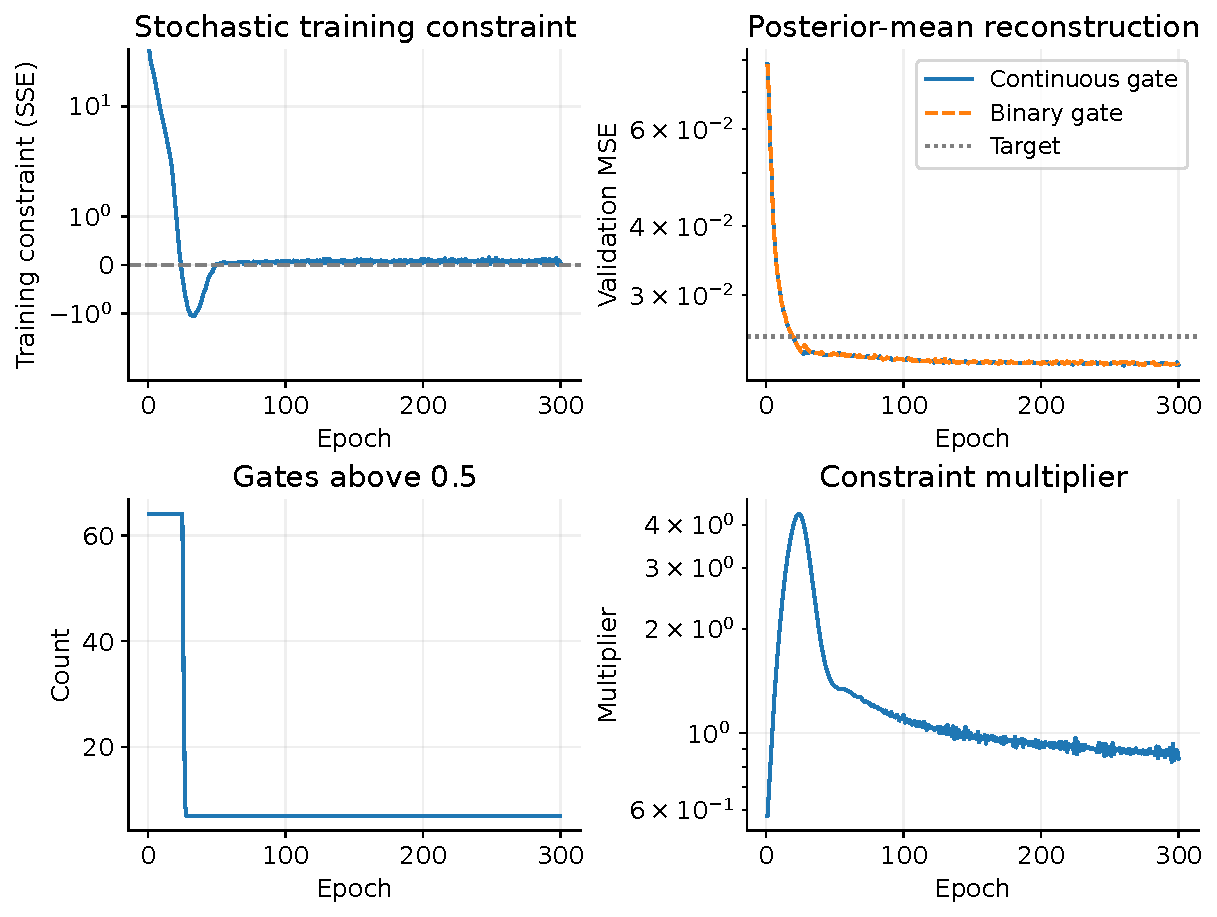
\includegraphics[width=\textwidth]{results/figures/MAKE51/native_hc.pdf}
\caption{New MNIST hard-concrete implementation diagnostic, seed 42,
300 epochs. The training constraint uses sampled latent variables and
gates; validation uses posterior means. Gate count and multiplier are
shown alongside constraint and reconstruction trajectories.
This is one local HC run, not an original ARM reproduction.}
\label{fig:hc}
\end{figure}

The ARD adaptation reserves the first 10\% (1800 examples) of its
training array for prior estimation and trains on the remainder.
It updates $p_j=\operatorname{mean}(\mu_j^2+\sigma_j^2)$ every ten
epochs and after training, clipping to $[10^{-6},10^6]$.
This uses analytic posterior second moments in a fixed subset, rather
than a periodically resampled encoded-data pool. Selection training uses
reconstruction plus Gaussian KL at unit weight. On the first 512
training examples it computes
\begin{equation}
 w_j=\operatorname{mean}_{x,k}
 [g_k(\mu(x)+\sqrt{p_j}e_j)-g_k(\mu(x))]^2,
 \qquad q_j=w_jp_j,
 \label{eq:ardlocal}
\end{equation}
and keeps the smallest number of descending scores reaching 99\% of
their total. The finite difference is not divided by its squared step.
Locally it already contains a factor $p_j$, so multiplication by $p_j$
again differs from a Jacobian-squared times variance score. The stored
counts are therefore labelled an \emph{ARD adaptation}; this difference
cannot be removed by correcting the prose. The Gaussian approximation
alone is not an original-source deviation. Identical relevance arrays
and counts across contexts are checked in the numerical audit; they
represent repeated fixed settings, not a $\beta$ sweep.

The stored $q_j$ and $p_j$ are sufficient to undo the extra finite-step
factor without access to the checkpoint. With $h_j=\sqrt{p_j}$, the
correctly normalized finite-step score is
\begin{equation}
 \widetilde q_j
 =p_j\,\operatorname{mean}_{x,k}
 \left[\frac{g_k(\mu+h_je_j)-g_k(\mu)}{h_j}\right]^2
 =\frac{q_j}{p_j}.
 \label{eq:ardcorrected}
\end{equation}
All saved $p_j$ are positive. We recompute the cumulative 99\% count
and transfer it using the same nearest-grid rule. Table~\ref{tab:ard_normalized}
shows that CIFAR-10 changes from a mean raw count 14.2 to 26.0,
mapping to width 24 and attaining $Q$ in all five trials. This is an
algebraic correction of the finite-step readout up to stored numerical
precision. Its
possibly large steps and altered prior updates remain; it is not
an exact-Jacobian or original-ARD benchmark.
\begin{table}[H]
\caption{Corrected finite-step relevance readout from saved scores and prior variances at the primary context. The same stored perturbations are normalized by their squared step before variance weighting; no new ARD training is involved. This validates an algebraic readout correction, not exact Jacobian relevance or the source training procedure. Test MSE $\times10^3$ is for transferred ordinary VAEs.}\label{tab:ard_normalized}
\small
\setlength{\tabcolsep}{3pt}
\begin{tabular*}{\textwidth}{@{\extracolsep{\fill}}lccccc@{}}
\toprule
Dataset & Old raw & Corrected raw & Grid width & $Q$ & Test MSE \\
\midrule
MNIST & $6.0 \pm 0.0$ & $6.2 \pm 0.4$ & $6.0 \pm 0.0$ & 5/5 & $22.05 \pm 0.17$ \\
Fashion-MNIST & $3.8 \pm 0.4$ & $4.0 \pm 0.0$ & $4.0 \pm 0.0$ & 5/5 & $19.06 \pm 0.25$ \\
dSprites & $9.2 \pm 1.5$ & $10.6 \pm 0.5$ & $10.0 \pm 0.0$ & 0/5 & $1.47 \pm 0.05$ \\
CIFAR-10 & $14.2 \pm 0.4$ & $26.0 \pm 0.0$ & $24.0 \pm 0.0$ & 5/5 & $15.36 \pm 0.13$ \\
\bottomrule\end{tabular*}
\end{table}


The additional exact-Jacobian runs are reported separately in
Section~\ref{sec:newpruning}; they do not replace these historical records.

The FONDUE description-based classifier was checked against the public
repository \url{https://github.com/bonheml/VAE_learning_dynamics} at
commit \texttt{f6d6e66b536bcbe635392d3438338949d4dc8730}. The local
implementation uses the stated posterior-variance categories with one
exponentiation and TwoNN; equivalence to the public execution path and
the original experiment configuration is not asserted. As a historical
reference, the source reports dSprites selection $12.2\pm0.4$ at one
epoch~\cite{bonheme2022fondue}, versus $4.2\pm0.4$ here at $\beta=1$.
This unmatched-setting difference is not proof of an implementation
error, nor a reproduction of the original benchmark.
A separate control-flow check replays the source algorithm's
lower/upper-bound updates on the archived ID-gap sequence: all 100
FONDUE paths and returned widths agree with that pseudocode and
terminate normally. This verifies the search update logic on those
inputs; it does not validate the estimator implementation, training
framework parity or the published benchmark. Its row-level results
are included as \path{results/make51/fondue_control_flow.json}.

\subsection{Threshold-Only and Quality-Margin Analyses}\label{app:sensitivity}
The retrospective predictive analysis uses Python 3.11.11,
NumPy 2.3.2 and scikit-learn 1.7.1. Table~\ref{tab:saturation}
documents probability saturation in this reconstruction. The original
predictor's complete environment and row-level probabilities were not
saved, so its exact floating-point results cannot be verified from the
summary alone. Row-level decision scores and probabilities for the
current reconstruction are saved in \path{results/make51/au_predictions.csv}.
\begin{table}[H]
\caption{Numerical probability saturation in the current predictor reconstruction. Entries count predictions rounded to exactly one, before AUROC calculation. Decision scores preserve ordering among these rows.}\label{tab:saturation}
\small
\setlength{\tabcolsep}{3.5pt}
\begin{tabular*}{\textwidth}{@{\extracolsep{\fill}}lccc@{}}
\toprule
Evaluation condition & Base & Base + AU & Base + random \\
\midrule
dSprites & 55/55 & 44/55 & 49/55 \\
Fashion-MNIST & 0/55 & 0/55 & 0/55 \\
CIFAR-10 & 45/45 & 40/45 & 36/45 \\
\bottomrule
\end{tabular*}
\end{table}


The main AU-threshold figure uses identical checkpoints for all three
$\delta$ values. Across the full ladder, the fractions of CIFAR-10
grid/seed candidates with AU equal to capacity are given below.
These counts use ten widths and five seeds per $\beta$; their rows are
not 50 independent datasets.
\begin{table}[H]
\caption{CIFAR-10 (Gaussian): percentage of the 50 width/seed candidates with AU equal to capacity. Thresholds are re-read on the same checkpoints within each column.}\label{tab:delta_rates}
\small
\setlength{\tabcolsep}{3.5pt}
\begin{tabular*}{\textwidth}{@{\extracolsep{\fill}}lccccc@{}}
\toprule
$\delta$ & $\beta=.25$ & $.5$ & $1$ & $2$ & $4$ \\
\midrule
0.001 & 100 & 100 & 100 & 98 & 60 \\
0.01 & 60 & 50 & 36 & 22 & 10 \\
0.1 & 48 & 38 & 32 & 20 & 10 \\
\bottomrule
\end{tabular*}
\end{table}


For a separate retrospective quality-margin check, the complete cached
grid at $\beta=1$ is held fixed and the smallest satisfying width is read
out for each margin, without retraining or changing the anchor.
Table~\ref{tab:margin} reports this full-grid criterion, not the path or
cost of any restricted-window selector. No FONDUE-threshold or ARD-99\%
sensitivity training was executed, so no response of those rules to their
own readout thresholds is claimed.
\begin{table}[H]
\caption{Smallest quality-satisfying cached width at $\beta=1$ as relative margin changes; five seed means $\pm$ SD. The absolute floor 0.001 times validation variance remains fixed. Gaussian likelihood except Bernoulli dSprites.}\label{tab:margin}
\footnotesize
\setlength{\tabcolsep}{3.5pt}
\begin{tabular*}{\textwidth}{@{\extracolsep{\fill}}lccccc@{}}
\toprule
Dataset & 1\% & 5\% & 10\% & 25\% & 50\% \\
\midrule
MNIST & $6.0 \pm 0.0$ & $6.0 \pm 0.0$ & $6.0 \pm 0.0$ & $4.0 \pm 0.0$ & $4.0 \pm 0.0$ \\
Fashion-MNIST & $4.0 \pm 0.0$ & $4.0 \pm 0.0$ & $4.0 \pm 0.0$ & $4.0 \pm 0.0$ & $2.0 \pm 0.0$ \\
dSprites & $51.2 \pm 17.5$ & $36.0 \pm 16.5$ & $20.0 \pm 4.0$ & $12.0 \pm 0.0$ & $9.6 \pm 0.9$ \\
CIFAR-10 & $41.6 \pm 8.8$ & $32.0 \pm 0.0$ & $24.0 \pm 0.0$ & $16.0 \pm 0.0$ & $16.0 \pm 0.0$ \\
\bottomrule
\end{tabular*}
\end{table}


\section{Synthetic Scale and Ablation Diagnostic}\label{app:synthetic}
Swiss-roll points are $(t\cos t,h,t\sin t)$ with
$t\sim U[1.5\pi,4.5\pi]$ and $h\sim U[0,1]$. Torus points are
$((3+\cos\phi)\cos\theta,(3+\cos\phi)\sin\theta,\sin\phi)$ with
independent angles uniform on $[0,2\pi]$. Each has 5000 examples,
generation seed zero, and independent Gaussian coordinate noise with
SD 0.01. The first 4500 are used for fitting and the remaining 500 for
the reported diagnostic. Per-coordinate standardisation in the stored
experiment was fitted to all 5000 before splitting. This is disclosed
as preprocessing leakage; the results are descriptive, not clean
held-out test estimates.

The FC VAE uses widths 128 and 64, reversed in its decoder, ReLU hidden
activations, a linear output, Adam at $10^{-3}$, batch 128, 300 epochs,
$\beta=1$ and seeds 42, 123 and 777. At the last checkpoint, coordinates
with posterior-mean variance at most 0.01 on the 500 diagnostic examples
are zeroed and MSE is recomputed on those same examples.
Table~\ref{tab:synthetic} reports the standardized runs. There is no
separate test set in this stored experiment.

\begin{table}[H]
\caption{Synthetic scale/ablation diagnostic, Gaussian likelihood, $\beta=1$, $\delta=0.01$, three training seeds. Data were standardized before the split; these are descriptive validation results, not leakage-free generalization estimates. Changes are mean per-run relative MSE changes (\%).}\label{tab:synthetic}
\footnotesize
\setlength{\tabcolsep}{3.5pt}
\begin{tabular*}{\textwidth}{@{\extracolsep{\fill}}lccccc@{}}
\toprule
Data & $m$ & AU & MSE before & MSE after & Change \\
\midrule
Swiss roll & 1 & $1.0 \pm 0.0$ & $0.3511 \pm 0.0267$ & $0.3511 \pm 0.0267$ & +0.000 \\
Swiss roll & 2 & $2.0 \pm 0.0$ & $0.1997 \pm 0.0177$ & $0.1997 \pm 0.0177$ & +0.000 \\
Swiss roll & 3 & $3.0 \pm 0.0$ & $0.1407 \pm 0.0018$ & $0.1407 \pm 0.0018$ & +0.000 \\
Swiss roll & 4 & $3.0 \pm 0.0$ & $0.1404 \pm 0.0136$ & $0.1406 \pm 0.0135$ & +0.147 \\
Swiss roll & 6 & $3.0 \pm 0.0$ & $0.1365 \pm 0.0023$ & $0.1368 \pm 0.0022$ & +0.183 \\
Swiss roll & 8 & $3.0 \pm 0.0$ & $0.1437 \pm 0.0089$ & $0.1440 \pm 0.0089$ & +0.165 \\
Torus & 1 & $1.0 \pm 0.0$ & $0.3217 \pm 0.0163$ & $0.3217 \pm 0.0163$ & +0.000 \\
Torus & 2 & $2.0 \pm 0.0$ & $0.1654 \pm 0.0242$ & $0.1654 \pm 0.0242$ & +0.000 \\
Torus & 3 & $3.0 \pm 0.0$ & $0.1083 \pm 0.0036$ & $0.1083 \pm 0.0036$ & +0.000 \\
Torus & 4 & $3.0 \pm 0.0$ & $0.1124 \pm 0.0050$ & $0.1124 \pm 0.0050$ & +0.063 \\
Torus & 6 & $3.0 \pm 0.0$ & $0.1095 \pm 0.0035$ & $0.1096 \pm 0.0035$ & +0.107 \\
Torus & 8 & $3.0 \pm 0.0$ & $0.1104 \pm 0.0069$ & $0.1105 \pm 0.0069$ & +0.156 \\
\bottomrule
\end{tabular*}
\end{table}


Both noise-free generating surfaces have intrinsic dimension two and
are represented here in three ambient coordinates. A Swiss-roll patch
does not thereby have minimum embedding dimension three. Observing
three active coordinates under this loss is not a topological theorem.
The earlier manuscript said its synthetic coordinates were standardized;
the implementation audit found a mismatch between that description and
the executed preprocessing. On the unstandardized Swiss roll the height
coordinate has much smaller variance than the other coordinates, making
its omission inexpensive in squared error. This scale observation does
not alone prove the complete causal explanation of every earlier AU
result.

\section{New MNIST Model Records}\label{app:newmodels}
The new experiment uses all twelve declared widths, training seed 42,
and the original split reconstructed from its fixed seeds. The model
architecture and objective match the ordinary MNIST protocol, while
the CPU environment differs from the archived CUDA runs.
Table~\ref{tab:mcgrid} gives every proxy-selected checkpoint's validation
criteria. MC SE refers only to evaluation noise over posterior draws.
The frozen capacity-choice file precedes final test evaluation.
Weights, epoch curves and draw-wise ELBO means are included in the
reviewer supplement. No between-training-seed confidence interval is
inferred from this one-seed validation.
\begin{table}[H]
\caption{Complete newly trained MNIST grid, seed 42, $\beta=1$, Gaussian likelihood. Epoch selected by the deterministic proxy; stop is the actual final training epoch. Proxy omits the Gaussian constant and posterior expectation; MC ELBO includes both. MSE $\times10^3$.}\label{tab:mcgrid}
\small
\setlength{\tabcolsep}{3pt}
\begin{tabular*}{\textwidth}{@{\extracolsep{\fill}}rrrrrc@{}}
\toprule
Width & Epoch & Stop & Val. MSE & Proxy & MC ELBO $\pm$ SE \\
\midrule
2 & 81 & 111 & 37.406 & $-34.647$ & $-484.386 \pm 0.009$ \\
4 & 85 & 115 & 27.840 & $-29.304$ & $-480.108 \pm 0.009$ \\
6 & 169 & 199 & 22.343 & $-26.696$ & $-478.174 \pm 0.010$ \\
8 & 73 & 103 & 22.417 & $-26.544$ & $-478.285 \pm 0.009$ \\
10 & 70 & 100 & 22.954 & $-26.663$ & $-478.627 \pm 0.009$ \\
12 & 196 & 226 & 20.983 & $-26.055$ & $-478.067 \pm 0.012$ \\
16 & 107 & 137 & 23.030 & $-26.774$ & $-478.592 \pm 0.009$ \\
20 & 144 & 174 & 21.327 & $-26.156$ & $-478.134 \pm 0.010$ \\
24 & 132 & 162 & 22.977 & $-26.956$ & $-478.664 \pm 0.008$ \\
32 & 136 & 166 & 23.402 & $-27.042$ & $-478.869 \pm 0.012$ \\
48 & 114 & 144 & 24.177 & $-27.411$ & $-479.310 \pm 0.013$ \\
64 & 217 & 247 & 22.930 & $-26.946$ & $-479.043 \pm 0.011$ \\
\bottomrule\end{tabular*}
\end{table}


\begin{figure}[!htbp]
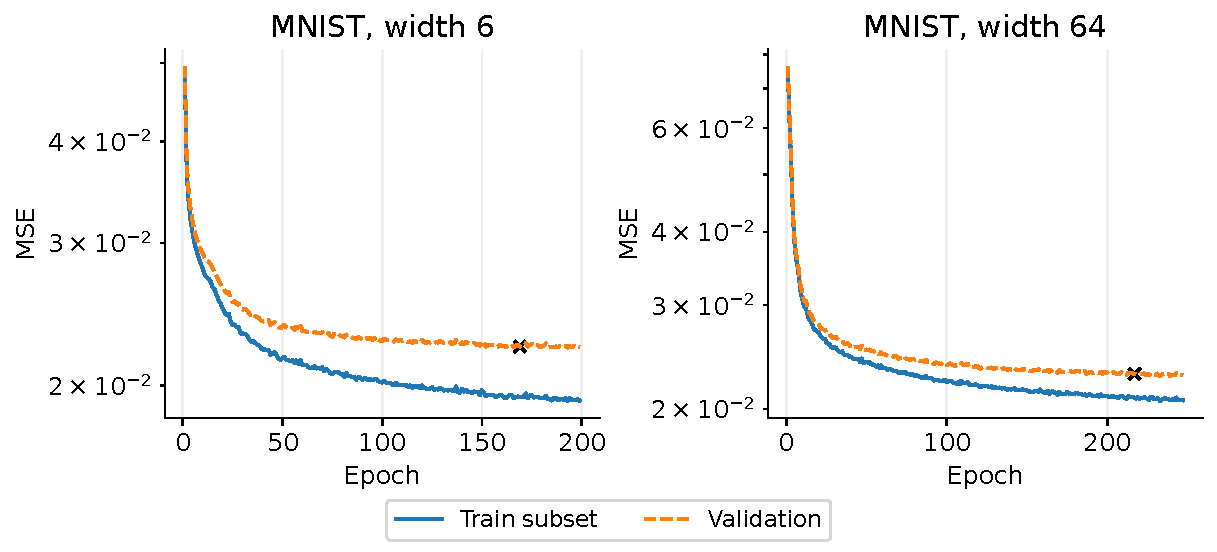
\includegraphics[width=\textwidth]{results/figures/MAKE51/new_mnist_curves.pdf}
\caption{New MNIST seed-42 train/validation MSE at widths six and 64,
Gaussian likelihood and $\beta=1$. Training curves use a fixed
2000-example subset; validation uses all 2000 held-out examples.
Black crosses mark proxy-selected epochs. These are new saved runs,
not reconstructed train curves for the historical CUDA checkpoints.}
\label{fig:newcurves}
\end{figure}

\section{Additional GPU Validation Records}\label{app:gpu}
Table~\ref{tab:newcounts} compares historical and additional readouts.
The ARM dSprites mean is 54.0 rather than the historical HC count of 64.
The historical unnormalised CIFAR-10 ARD count was 14.2, but its
normalisation audit had already changed it to 26.0
(Table~\ref{tab:ard_normalized}). New exact-Jacobian counts are close
to that corrected result. Changes in training and prior updates prevent
attributing the full difference from 14.2 solely to the Jacobian calculation.
\begin{table}[H]
\caption{Raw dimension readouts: historical HC and unnormalized finite-step ARD (five seeds) versus new ARM and exact-Jacobian ARD (three seeds). Mean $\pm$ sample SD. Different training and readout settings prevent attributing every difference to the estimator alone. The corrected historical finite-step ARD results are retained in Table~\ref{tab:ard_normalized}.}\label{tab:newcounts}
\footnotesize
\setlength{\tabcolsep}{3pt}
\begin{tabular*}{\textwidth}{@{\extracolsep{\fill}}lccccc@{}}
\toprule
Dataset & HC ($n=5$) & ARM ($n=3$) & Old ARD ($n=5$) & Exact, zero & Exact, sample \\
\midrule
MNIST & $7.2 \pm 0.4$ & $7.7 \pm 0.6$ & $6.0 \pm 0.0$ & $6.0 \pm 0.0$ & $6.0 \pm 0.0$ \\
Fashion-MNIST & $4.2 \pm 0.4$ & $4.7 \pm 0.6$ & $3.8 \pm 0.4$ & $4.0 \pm 0.0$ & $4.0 \pm 0.0$ \\
dSprites & $64.0 \pm 0.0$ & $54.0 \pm 7.2$ & $9.2 \pm 1.5$ & $9.0 \pm 0.0$ & $9.7 \pm 0.6$ \\
CIFAR-10 & $20.0 \pm 1.0$ & $21.0 \pm 2.6$ & $14.2 \pm 0.4$ & $26.7 \pm 0.6$ & $26.3 \pm 0.6$ \\
\bottomrule\end{tabular*}
\end{table}


The new records comprise three seeds per dataset for ARM and for each
ARD variance-update setting. Gate bins in Table~\ref{tab:armgates} and
the individual constraint trajectories in Figure~\ref{fig:armconstraints}
show why a thresholded dimension count is insufficient to diagnose
successful pruning. In particular, dSprites does not approach a decisive
binary gate configuration or a satisfied constraint.
\begin{table}[H]
\caption{ARM gate probabilities after 300 epochs. Mid denotes $0.1\le p\le0.9$; the other bins use strict inequalities. Expected is $\sum_j p_j$; count uses $p_j>0.5$. No dSprites gate reaches either extreme, so its threshold count should not be read as a stable binary architecture.}\label{tab:armgates}
\small
\setlength{\tabcolsep}{3pt}
\begin{tabular*}{\textwidth}{@{\extracolsep{\fill}}lrrrrrr@{}}
\toprule
Dataset & Seed & $p<0.1$ & Mid & $p>0.9$ & Expected & Count \\
\midrule
MNIST & 42 & 56 & 0 & 8 & 8.33 & 8 \\
MNIST & 123 & 56 & 1 & 7 & 8.11 & 8 \\
MNIST & 777 & 57 & 0 & 7 & 7.34 & 7 \\
Fashion-MNIST & 42 & 59 & 0 & 5 & 5.32 & 5 \\
Fashion-MNIST & 123 & 59 & 0 & 5 & 5.30 & 5 \\
Fashion-MNIST & 777 & 60 & 0 & 4 & 4.35 & 4 \\
dSprites & 42 & 0 & 64 & 0 & 32.08 & 52 \\
dSprites & 123 & 0 & 64 & 0 & 32.20 & 62 \\
dSprites & 777 & 0 & 64 & 0 & 32.05 & 48 \\
CIFAR-10 & 42 & 236 & 1 & 19 & 25.65 & 19 \\
CIFAR-10 & 123 & 230 & 3 & 23 & 30.27 & 24 \\
CIFAR-10 & 777 & 235 & 1 & 20 & 26.18 & 20 \\
\bottomrule\end{tabular*}
\end{table}


\begin{figure}[!htbp]
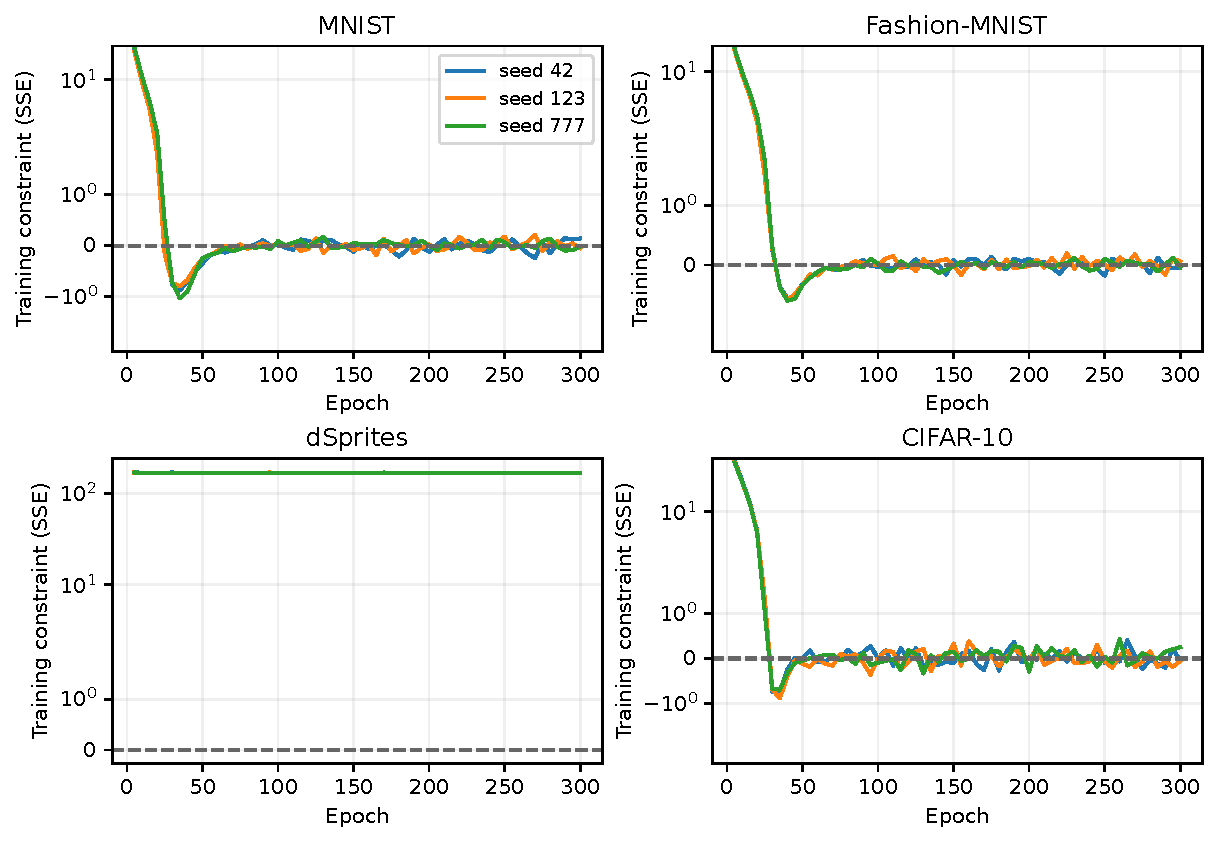
\includegraphics[width=\textwidth]{results/figures/MAKE52/arm_constraints.pdf}
\caption{Moving-average stochastic training constraint for each new ARM
seed, recorded every five epochs. Zero is the constraint boundary;
negative values satisfy it. A symmetric logarithmic vertical scale
accommodates large positive violations and negative values. These
trajectories are distinct from deterministic validation-target attainment.}
\label{fig:armconstraints}
\end{figure}

Figures~\ref{fig:armcurves} and~\ref{fig:ardcurves} report evaluation-mode
reconstruction curves for all four datasets. They describe the supplied
300-epoch runs; a visually flat curve does not certify an optimum.
The ARD figure uses zero-centre variance updates. All 24 ARD curve
records, including the sample-centred variant, are in the supplement.

\begin{figure}[!htbp]
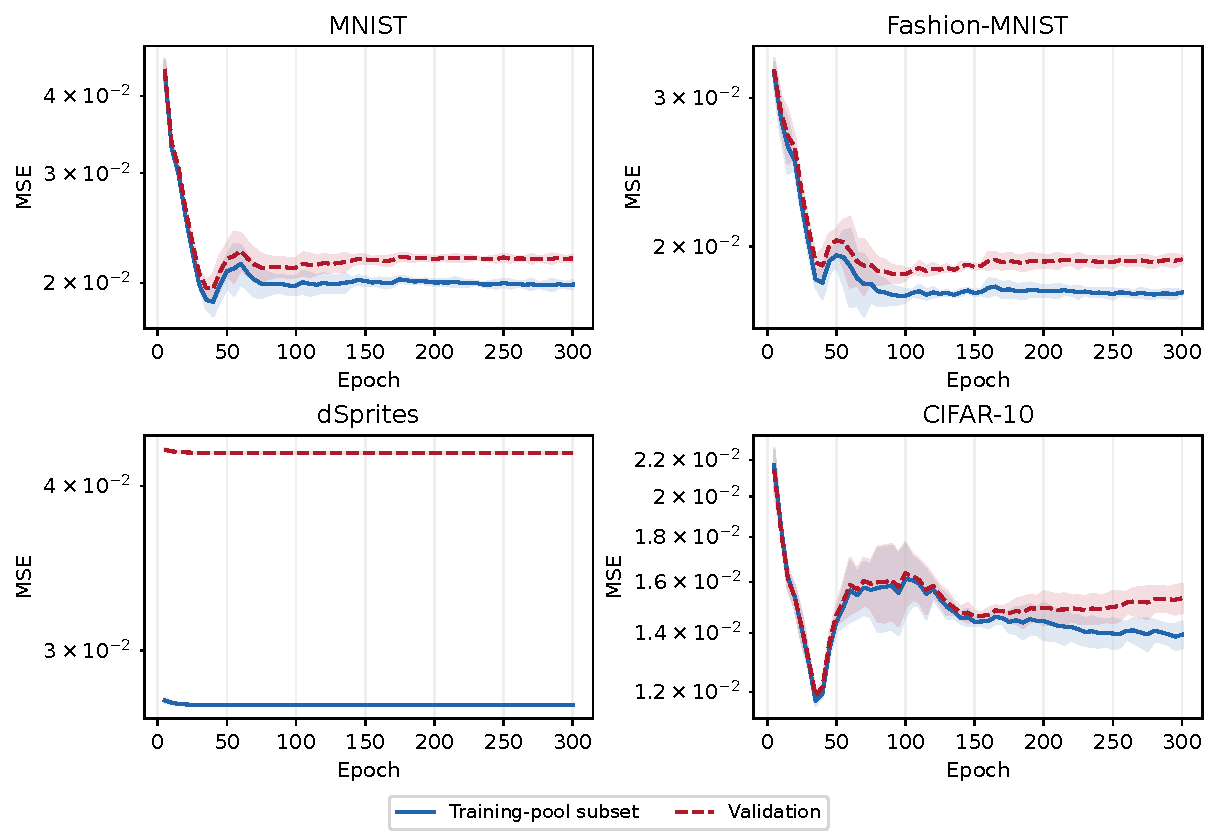
\includegraphics[width=\textwidth]{results/figures/MAKE52/arm_curves.pdf}
\caption{Native ARM posterior-mean MSE with the current binary gate mask,
evaluated every five epochs on a 2000-example training subset and the
validation split. Lines and shading are mean and sample SD over three
seeds. Vertical axes are logarithmic; a shaded lower bound is clipped
above zero for display. These curves do not reconstruct missing historical
ordinary-VAE training records.}
\label{fig:armcurves}
\end{figure}

\begin{figure}[!htbp]
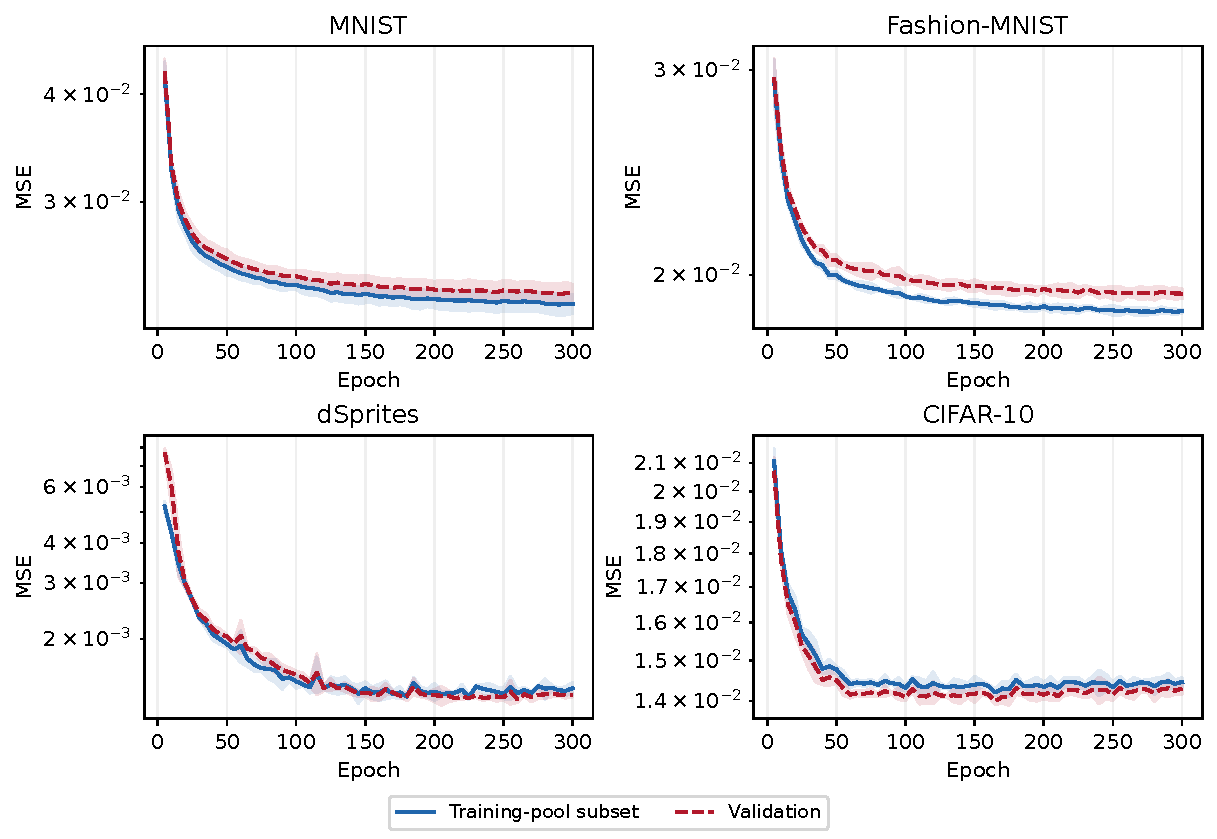
\includegraphics[width=\textwidth]{results/figures/MAKE52/ard_curves.pdf}
\caption{Full-width ARD posterior-mean MSE with zero-centre variance
updates, evaluated every five epochs. Mean and sample SD over three
seeds; logarithmic vertical axes. The 2000-example training-pool subset
includes 1800 examples reserved for prior updates and 200 used in
parameter-gradient training, so its curve is not a pure training-fit
estimate. No native pruning is applied in these evaluations.}
\label{fig:ardcurves}
\end{figure}

Table~\ref{tab:newtest} reports held-out test reconstruction at the
fixed final native models and transferred ordinary widths. Selection
uses the constraint or validation-based relevance readout, not these
test metrics. The full-model ARD column is deliberately distinguished
from quality at a selected native dimension.
\begin{table}[H]
\caption{Test MSE ($\times10^3$), mean $\pm$ sample SD over three seeds. ARM native evaluation uses a binary gate mask and posterior mean. ARD native evaluation is the unpruned full-width model. Transferred ordinary VAEs are reused from the archived candidate cache; their test summaries did not select the new raw counts.}\label{tab:newtest}
\small
\setlength{\tabcolsep}{3pt}
\begin{tabular*}{\textwidth}{@{\extracolsep{\fill}}llcc@{}}
\toprule
Dataset & Implementation & Native/full & Transferred \\
\midrule
MNIST & ARM & $21.35 \pm 0.25$ & $21.22 \pm 0.79$ \\
MNIST & ARD zero & $22.97 \pm 0.53$ & $22.15 \pm 0.14$ \\
MNIST & ARD sample & $23.17 \pm 0.17$ & $22.15 \pm 0.14$ \\
Fashion-MNIST & ARM & $19.01 \pm 0.23$ & $18.94 \pm 0.23$ \\
Fashion-MNIST & ARD zero & $18.97 \pm 0.17$ & $18.94 \pm 0.23$ \\
Fashion-MNIST & ARD sample & $19.17 \pm 0.15$ & $18.94 \pm 0.23$ \\
dSprites & ARM & $42.10 \pm 0.00$ & $1.17 \pm 0.04$ \\
dSprites & ARD zero & $1.32 \pm 0.01$ & $1.86 \pm 0.09$ \\
dSprites & ARD sample & $1.32 \pm 0.06$ & $1.61 \pm 0.30$ \\
CIFAR-10 & ARM & $15.60 \pm 0.59$ & $16.74 \pm 1.21$ \\
CIFAR-10 & ARD zero & $14.55 \pm 0.13$ & $15.42 \pm 0.13$ \\
CIFAR-10 & ARD sample & $14.64 \pm 0.24$ & $15.42 \pm 0.13$ \\
\bottomrule\end{tabular*}
\end{table}


Table~\ref{tab:newcost} reports logged duration components. The source
records identify an NVIDIA GPU and the software environment. Training
intervals include periodic evaluation; the ARD initial and final prior
updates and final native evaluation are not included in the listed
training/Jacobian intervals. Jacobian timing pertains to 100 validation
examples and the particular architecture. Missing reference, anchor,
transfer and evaluation components preclude interpreting these numbers
as complete selector costs or combining them with historical CPU ID time.
\begin{table}[H]
\caption{Logged duration components for new GPU pruning runs, seconds, mean $\pm$ sample SD over three seeds. Training loop includes periodic train/validation evaluations. ARM post-evaluation covers final native evaluations; ARD did not separately time them (NR). Anchor, transferred-candidate and other missing costs are not included here. These intervals are not complete end-to-end selector costs.}\label{tab:newcost}
\small
\setlength{\tabcolsep}{3pt}
\begin{tabular*}{\textwidth}{@{\extracolsep{\fill}}llccc@{}}
\toprule
Dataset & Implementation & Training loop & Jacobian & Post-evaluation \\
\midrule
MNIST & ARM & $197.8 \pm 2.2$ & --- & $0.043 \pm 0.000$ \\
MNIST & ARD, zero & $87.3 \pm 0.3$ & $0.011 \pm 0.000$ & NR \\
MNIST & ARD, sample & $87.1 \pm 0.7$ & $0.012 \pm 0.002$ & NR \\
Fashion-MNIST & ARM & $197.8 \pm 1.5$ & --- & $0.043 \pm 0.000$ \\
Fashion-MNIST & ARD, zero & $88.2 \pm 0.5$ & $0.011 \pm 0.000$ & NR \\
Fashion-MNIST & ARD, sample & $88.0 \pm 0.3$ & $0.012 \pm 0.002$ & NR \\
dSprites & ARM & $664.8 \pm 0.3$ & --- & $1.264 \pm 0.001$ \\
dSprites & ARD, zero & $299.2 \pm 0.0$ & $10.830 \pm 0.169$ & NR \\
dSprites & ARD, sample & $299.2 \pm 0.2$ & $11.047 \pm 0.712$ & NR \\
CIFAR-10 & ARM & $328.4 \pm 0.3$ & --- & $0.570 \pm 0.001$ \\
CIFAR-10 & ARD, zero & $146.2 \pm 0.1$ & $6.968 \pm 0.452$ & NR \\
CIFAR-10 & ARD, sample & $146.1 \pm 0.1$ & $7.505 \pm 0.171$ & NR \\
\bottomrule\end{tabular*}
\end{table}


\subsection{Native Masking and Decoder Adaptation}
Tables~\ref{tab:ardprunedseeds} and~\ref{tab:ardprunedtest} provide
the seed-level validation records and held-out test summaries for the
four native-pruning conditions. The selected counts match the preceding
sample-centred runs. Their unpruned validation/test MSEs are also
identical, so the repeated baseline is not extra independent evidence.
The dSprites test means follow the validation pattern: 0.00132 before
masking, 0.00294 after masking and 0.00178 after decoder adaptation.
\begin{table}[H]
\caption{Per-seed native-pruning validation MSE $\times10^3$. Count is the relevance-selected axis count; Grid is the transferred ordinary-VAE width. Full, Mask and Adapt use posterior means. Sampled mask averages MSE over 32 posterior draws before adaptation; it is neither an ELBO nor a comparison under a sampled-anchor target. Exact masks and model checkpoints were not saved.}\label{tab:ardprunedseeds}
\footnotesize
\setlength{\tabcolsep}{3pt}
\begin{tabular*}{\textwidth}{@{\extracolsep{\fill}}lrrrrrrr@{}}
\toprule
Dataset & Seed & Count & Grid & Full & Mask & Adapt & Sampled mask \\
\midrule
MNIST & 42 & 6 & 6 & $23.762$ & $23.772$ & $23.445$ & $27.040$ \\
MNIST & 123 & 6 & 6 & $23.669$ & $23.681$ & $23.454$ & $27.050$ \\
MNIST & 777 & 6 & 6 & $23.410$ & $23.420$ & $23.175$ & $26.896$ \\
Fashion-MNIST & 42 & 4 & 4 & $19.336$ & $19.340$ & $19.158$ & $21.573$ \\
Fashion-MNIST & 123 & 4 & 4 & $19.452$ & $19.456$ & $19.248$ & $21.732$ \\
Fashion-MNIST & 777 & 4 & 4 & $19.496$ & $19.496$ & $19.176$ & $21.563$ \\
dSprites & 42 & 10 & 10 & $1.393$ & $3.317$ & $1.893$ & $3.611$ \\
dSprites & 123 & 10 & 10 & $1.278$ & $2.783$ & $1.727$ & $3.084$ \\
dSprites & 777 & 9 & 8 & $1.327$ & $2.945$ & $1.859$ & $3.223$ \\
CIFAR-10 & 42 & 26 & 24 & $14.668$ & $15.109$ & $14.817$ & $17.584$ \\
CIFAR-10 & 123 & 26 & 24 & $14.192$ & $14.728$ & $14.671$ & $17.253$ \\
CIFAR-10 & 777 & 27 & 24 & $14.353$ & $14.835$ & $14.692$ & $17.392$ \\
\bottomrule\end{tabular*}
\end{table}


\begin{table}[H]
\caption{Native-pruning test MSE $\times10^3$, mean $\pm$ sample SD across three seeds. All columns use posterior-mean reconstruction. Conditions match Table~\ref{tab:ardpruned}; test metrics do not choose the axes or the fixed adaptation budget.}\label{tab:ardprunedtest}
\small
\setlength{\tabcolsep}{3pt}
\begin{tabular*}{\textwidth}{@{\extracolsep{\fill}}lcccc@{}}
\toprule
Dataset & Full & Mask & Adapt & Transfer \\
\midrule
MNIST & $23.17 \pm 0.17$ & $23.18 \pm 0.17$ & $22.90 \pm 0.14$ & $22.15 \pm 0.14$ \\
Fashion-MNIST & $19.17 \pm 0.15$ & $19.17 \pm 0.15$ & $18.93 \pm 0.08$ & $18.94 \pm 0.23$ \\
dSprites & $1.32 \pm 0.06$ & $2.94 \pm 0.25$ & $1.78 \pm 0.07$ & $1.61 \pm 0.30$ \\
CIFAR-10 & $14.64 \pm 0.24$ & $15.14 \pm 0.19$ & $14.97 \pm 0.08$ & $15.42 \pm 0.13$ \\
\bottomrule\end{tabular*}
\end{table}


Table~\ref{tab:ardprunedcost} reports the two recorded timing intervals.
Unlike the earlier curve runs, the initial training interval has no
periodic evaluation and includes the final prior update. The initial
prior update, Jacobian evaluation, mask construction and final model
evaluations are outside the recorded intervals. Adding training and
adaptation times would therefore not give end-to-end pruning cost.
The supplied script defines the 300-epoch training and 30-epoch
adaptation protocol, but its JSON lacks epoch counters and trajectories.
These settings are documented from the script and internal specification,
not independently recovered from a saved training trace.
\begin{table}[H]
\caption{Partial durations for native-pruning runs, seconds, mean $\pm$ sample SD across three seeds. Training includes its final prior update but excludes the initial one. Adaptation times only the 30-epoch decoder loop. Jacobian/mask construction, final evaluations, anchor and transfer training are excluded and are not separately timed in this run.}\label{tab:ardprunedcost}
\small
\setlength{\tabcolsep}{3pt}
\begin{tabular*}{\textwidth}{@{\extracolsep{\fill}}lcc@{}}
\toprule
Dataset & Training interval & Decoder adaptation \\
\midrule
MNIST & $86.5 \pm 0.7$ & $5.9 \pm 0.1$ \\
Fashion-MNIST & $86.5 \pm 0.4$ & $5.9 \pm 0.0$ \\
dSprites & $289.0 \pm 0.3$ & $20.7 \pm 0.0$ \\
CIFAR-10 & $142.3 \pm 0.1$ & $10.8 \pm 0.0$ \\
\bottomrule\end{tabular*}
\end{table}


The recorded \texttt{elbo} and \texttt{val\_elbo} fields remain in the
unmodified raw files for provenance but are not used as native ELBO
measurements (Section~\ref{sec:gpuvalidation}), including the new masking
records. Native post-masking MSE is now recorded, but checkpoints and
selected-axis identities were not saved. The mask, inference outputs
and a corrected native likelihood therefore cannot be independently
re-evaluated from the summaries alone. The analytic ARM-gradient check
validates a component; it cannot replace those model-level records.


\section{Reproducibility Inventory and Remaining Records}\label{app:inventory}
The reaggregation entry point is
\path{src/make51/rebuild_review.py}; it reads saved JSON and configuration
files and writes numerical tables, six figures and the paired predictive
analysis from the historical records. The new search analysis is
\path{src/make51/replay_search.py}; the bounded model validation is
\path{src/make51/validate_models.py}. Its outputs are summarized by
\path{src/make51/summarize_validation.py}. The additional-run reaggregation is
\path{src/make52/summarize_revision.py}; native-pruning reaggregation is
\path{src/make53/summarize_native_pruning.py}, and manuscript assembly is
\path{src/make53/build_manuscript.py}. The generated main TeX embeds its
table contents and references the figure PDFs. Compile from the project
root with \texttt{pdflatex} repeatedly until references settle.
The accompanying \texttt{MAKE53\_reproducibility.zip} supplies the files,
not only this inventory. Its README distinguishes inexpensive
reaggregation from optional retraining, gives dependency versions and
lists unavailable historical artifacts. \texttt{MANIFEST.sha256}
identifies the included payload. The archive contains a fixed source
snapshot and is usable without access to a private repository.

\begin{table}[H]
\caption{Source-to-output map for the present revision. Directories are
relative to the project root; the supplement README gives individual
filenames and reaggregation commands.}
\label{tab:inventory}\footnotesize
\begin{tabularx}{\textwidth}{lX}\toprule
Evidence & File or directory \\\midrule
Configuration & \path{config/} \\
Historical method, trajectory and diagnostic records & \path{results/make49/} \\
Candidate metrics and latent variances & \path{results/make49/stage4_cache/} \\
Search, AU and historical audit summaries & \path{results/make51/} \\
Separate MNIST models and MC ELBO records & \path{results/make51/model_validation/} \\
Gated-start, ARM, ARD and native-masking raw records & \path{results/make52/} \\
Native-masking summaries and source hashes & \path{results/make53/} \\
Historical and additional training code & \path{src/make49/}; \path{src/make52/} \\
Historical and additional reaggregation & \path{src/make51/}; \path{src/make53/} \\
English manuscript templates & \path{src/make53/} \\
Japanese translation and verification & \path{src/nn53/}; \path{results/nn53/} \\
English figures & \path{results/figures/MAKE51/}; \path{results/figures/MAKE52/} \\
Japanese figures & \path{results/figures/NN53/} \\
\bottomrule\end{tabularx}
\end{table}

Method-level row identifiers are
(dataset, method, candidate seed, $\beta$ or context). Candidate keys
also contain width, requested epochs and stopping option. Every
configuration/dataset--method--context cell in the main method archive
has five seeds; this is checked during reaggregation. The ARD repetition
does not create five distinct selection-weight conditions. Individual
early off-grid cache entries are not all retained, although their final
metrics and training traces remain in the method records. The original
test predictions, historical full model checkpoints and independent ID/evaluation
timings are not reconstructed from missing files.

The local change record documents the initial specification on
12 September; the switch to Bernoulli dSprites after collapse diagnostics;
the move of ID estimation from an impossible 10,000-example validation
sample to training data; trajectory runs without early stopping; and
the 13 September reference-width, run-accounting and degenerate-output
clarifications. The random-feature control was added after the primary
predictive analysis. In this revision, anchor-cost completion, paired AU
inference, quality-margin rereading and explicit implementation auditing
are retrospective. None is relabelled as a publicly preregistered test.
The 19 September local policies, threshold factorial, normalized ARD
readout and new one-seed validation were specified after those earlier
results. The supplement preserves their distinct specifications and
output locations.

The additional start-width and pruning records are separate retrospective
analyses. Reaggregation checks merged versus per-dataset files, three-seed
coverage, 300-epoch curve endpoints, raw count readouts, anchor targets
and transferred cache metrics. This verifies consistency of the supplied
records, not rerun equivalence of unavailable checkpoints. The new
native-masking audit additionally checks all 12 records against their
per-dataset files, the prior sample-centred full-model MSE/counts and
the transferred candidate cache; it recomputes $Q$ and paired summaries.
It cannot reconstruct the unsaved masks or checkpoint tensors.

\reftitle{References}
\begin{thebibliography}{999}

\bibitem{kingma2014vae}
Kingma, D.P.; Welling, M.
Auto-encoding variational Bayes.
In \textit{Proceedings of the 2nd International Conference on Learning
Representations (ICLR)}, Banff, AB, Canada, 14--16 April 2014.
arXiv:1312.6114. \url{https://doi.org/10.48550/arXiv.1312.6114}.

\bibitem{facco2017twonn}
Facco, E.; d'Errico, M.; Rodriguez, A.; Laio, A.
Estimating the intrinsic dimension of datasets by a minimal neighborhood
information.
\textit{Sci.\ Rep.} \textbf{2017}, \textit{7}, 12140.
\url{https://doi.org/10.1038/s41598-017-11873-y}.

\bibitem{levina2005mle}
Levina, E.; Bickel, P.J.
Maximum likelihood estimation of intrinsic dimension.
In \textit{Advances in Neural Information Processing Systems},
\textbf{2004}, \textit{17}.
\url{https://proceedings.neurips.cc/paper/2004/hash/74934548253bcab8490ebd74afed7031-Abstract.html}.

\bibitem{bonheme2022fondue}
Bonheme, L.; Grzes, M.
FONDUE: An algorithm to find the optimal dimensionality of the latent
representations of variational autoencoders.
arXiv \textbf{2022}, arXiv:2209.12806.
\url{https://doi.org/10.48550/arXiv.2209.12806}.

\bibitem{burda2016iwae}
Burda, Y.; Grosse, R.; Salakhutdinov, R.
Importance weighted autoencoders.
In \textit{Proceedings of the 4th International Conference on Learning
Representations (ICLR)}, San Juan, Puerto Rico, 2--4 May 2016.
arXiv:1509.00519. \url{https://doi.org/10.48550/arXiv.1509.00519}.

\bibitem{bonheme2023active}
Bonheme, L.; Grzes, M.
Be more active! Understanding the differences between mean and sampled
representations of variational autoencoders.
\textit{J. Mach. Learn. Res.} \textbf{2023}, \textit{24}(324), 1--30.
\url{https://jmlr.org/papers/v24/21-1145.html}.

\bibitem{deboom2020geco}
De Boom, C.; Wauthier, S.; Verbelen, T.; Dhoedt, B.
Dynamic narrowing of VAE bottlenecks using GECO and $L_0$ regularization.
arXiv \textbf{2020}, arXiv:2003.10901.
\url{https://doi.org/10.48550/arXiv.2003.10901}.

\bibitem{saha2025ardvae}
Saha, S.; Joshi, S.; Whitaker, R.
ARD-VAE: A statistical formulation to find the relevant latent dimensions
of variational autoencoders.
arXiv \textbf{2025}, arXiv:2501.10901.
\url{https://doi.org/10.48550/arXiv.2501.10901}.

\bibitem{tippingbishop1999ppca}
Tipping, M.E.; Bishop, C.M.
Probabilistic principal component analysis.
\textit{J.\ R.\ Stat.\ Soc.\ Ser.\ B} \textbf{1999}, \textit{61}, 611--622.
\url{https://doi.org/10.1111/1467-9868.00196}.

\bibitem{tenenbaum2000isomap}
Tenenbaum, J.B.; de Silva, V.; Langford, J.C.
A global geometric framework for nonlinear dimensionality reduction.
\textit{Science} \textbf{2000}, \textit{290}, 2319--2323.
\url{https://doi.org/10.1126/science.290.5500.2319}.

\bibitem{roweis2000lle}
Roweis, S.T.; Saul, L.K.
Nonlinear dimensionality reduction by locally linear embedding.
\textit{Science} \textbf{2000}, \textit{290}, 2323--2326.
\url{https://doi.org/10.1126/science.290.5500.2323}.

\bibitem{ceruti2014danco}
Ceruti, C.; Bassis, S.; Rozza, A.; Lombardi, G.; Casiraghi, E.;
Campadelli, P.
DANCo: An intrinsic dimensionality estimator exploiting angle and norm
concentration.
\textit{Pattern Recognit.} \textbf{2014}, \textit{47}, 2569--2581.
\url{https://doi.org/10.1016/j.patcog.2014.02.013}.

\bibitem{johnsson2015ess}
Johnsson, K.; Soneson, C.; Fontes, M.
Low bias local intrinsic dimension estimation from expected simplex
skewness.
\textit{IEEE Trans.\ Pattern Anal.\ Mach.\ Intell.} \textbf{2015},
\textit{37}, 196--202. \url{https://doi.org/10.1109/TPAMI.2014.2343220}.

\bibitem{costa2004geodesic}
Costa, J.A.; Hero, A.O.
Geodesic entropic graphs for dimension and entropy estimation in manifold
learning.
\textit{IEEE Trans.\ Signal Process.} \textbf{2004}, \textit{52},
2210--2221. \url{https://doi.org/10.1109/TSP.2004.831130}.

\bibitem{camastra2016intrinsic}
Camastra, F.; Staiano, A.
Intrinsic dimension estimation: Advances and open problems.
\textit{Inf.\ Sci.} \textbf{2016}, \textit{328}, 26--41.
\url{https://doi.org/10.1016/j.ins.2015.08.029}.

\bibitem{allegra2020data}
Allegra, M.; Facco, E.; Denti, F.; Laio, A.; Mira, A.
Data segmentation based on the local intrinsic dimension.
\textit{Sci.\ Rep.} \textbf{2020}, \textit{10}, 16449.
\url{https://doi.org/10.1038/s41598-020-72222-0}.

\bibitem{galka2022isolation}
Ga{\l}ka, {\L}.; Karczmarek, P.; Tokovarov, M.
Isolation Forest Based on Minimal Spanning Tree.
\textit{IEEE Access} \textbf{2022}, \textit{10}, 74175--74186.
\url{https://doi.org/10.1109/ACCESS.2022.3190505}.

\bibitem{ansuini2019intrinsic}
Ansuini, A.; Laio, A.; Macke, J.H.; Zoccolan, D.
Intrinsic dimension of data representations in deep neural networks.
In \textit{NeurIPS 2019}, Vol.~32, 2019. \url{https://proceedings.neurips.cc/paper_files/paper/2019/file/cfcce0621b49c983991ead4c3d4d3b6b-Paper.pdf}.

\bibitem{pope2021intrinsic}
Pope, P.; Zhu, C.; Abdelkader, A.; Goldblum, M.; Goldstein, T.
The intrinsic dimension of images and its impact on learning.
In \textit{ICLR 2021}, 2021. arXiv:2104.08894. \url{https://doi.org/10.48550/arXiv.2104.08894}.

\bibitem{rezende2018geco}
Rezende, D.J.; Viola, F.
Taming VAEs.
arXiv \textbf{2018}, arXiv:1810.00597.
\url{https://doi.org/10.48550/arXiv.1810.00597}.

\bibitem{louizos2018l0}
Louizos, C.; Welling, M.; Kingma, D.P.
Learning sparse neural networks through $L_0$ regularization.
In \textit{Proceedings of the 6th International Conference on Learning
Representations (ICLR)}, Vancouver, BC, Canada, 30 April--3 May 2018.
arXiv:1712.01312. \url{https://doi.org/10.48550/arXiv.1712.01312}.

\bibitem{obata2025manifold}
Obata, C.; Jin'no, K.
Analysis of the relationship between manifold structure and latent space
capacity of input data using VAE.
In \textit{Proceedings of the 2025 International Symposium on Nonlinear
Theory and Its Applications (NOLTA2025)}, Okinawa, Japan, 27--31 October
2025; pp. 32--35.
Publication record: \url{https://www.comm.tcu.ac.jp/nel/list_j_2025.html}
(accessed on 18 September 2026).

\bibitem{whitney1944}
Whitney, H.
The self-intersections of a smooth $n$-manifold in $2n$-space.
\textit{Ann. Math.} \textbf{1944}, \textit{45}, 220--246.
\url{https://doi.org/10.2307/1969265}.

\bibitem{lucas2019elbo}
Lucas, J.; Tucker, G.; Grosse, R.B.; Norouzi, M.
Don't blame the ELBO! A linear VAE perspective on posterior collapse.
In \textit{NeurIPS 2019}, Vol.~32, 2019. \url{https://proceedings.neurips.cc/paper/2019/file/7e3315fe390974fcf25e44a9445bd821-Paper.pdf}.

\bibitem{rolinek2019pca}
Rolinek, M.; Zietlow, D.; Martius, G.
Variational autoencoders pursue PCA directions (by accident).
In \textit{Proceedings of the IEEE/CVF Conference on Computer Vision and
Pattern Recognition (CVPR)}, Long Beach, CA, USA, 15--20 June 2019;
pp.\ 12406--12415. \url{https://doi.org/10.1109/CVPR.2019.01269}.

\bibitem{lecun1998}
LeCun, Y.; Bottou, L.; Bengio, Y.; Haffner, P.
Gradient-based learning applied to document recognition.
\textit{Proc.\ IEEE} \textbf{1998}, \textit{86}, 2278--2324.
\url{https://doi.org/10.1109/5.726791}.

\bibitem{xiao2017fashion}
Xiao, H.; Rasul, K.; Vollgraf, R.
Fashion-{MNIST}: A Novel Image Dataset for Benchmarking Machine Learning
Algorithms.
\textit{arXiv} \textbf{2017}, 1708.07747. \url{https://doi.org/10.48550/arXiv.1708.07747}.

\bibitem{krizhevsky2009learning}
Krizhevsky, A.
Learning multiple layers of features from tiny images.
\textit{Technical Report}; University of Toronto: Toronto, ON, Canada,
2009.

\bibitem{matthey2017dsprites}
Matthey, L.; Higgins, I.; Hassabis, D.; Lerchner, A.
dSprites: Disentanglement testing sprites dataset. 2017.
Available online: \url{https://github.com/google-deepmind/dsprites-dataset}
(accessed on 12 September 2026).

\bibitem{fu2019cyclical}
Fu, H.; Li, C.; Liu, X.; Gao, J.; Celikyilmaz, A.; Carin, L.
Cyclical annealing schedule: A simple approach to mitigating KL vanishing.
In \textit{Proceedings of NAACL-HLT 2019}, Minneapolis, MN, USA, 2019;
pp.~240--250. \url{https://doi.org/10.18653/v1/N19-1021}.

\end{thebibliography}
\end{document}
